\documentclass[twoside]{book}

% Packages required by doxygen
\usepackage{fixltx2e}
\usepackage{calc}
\usepackage{doxygen}
\usepackage{graphicx}
\usepackage[utf8]{inputenc}
\usepackage{makeidx}
\usepackage{multicol}
\usepackage{multirow}
\PassOptionsToPackage{warn}{textcomp}
\usepackage{textcomp}
\usepackage[nointegrals]{wasysym}
\usepackage[table]{xcolor}

% Font selection
\usepackage[T1]{fontenc}
\usepackage{mathptmx}
\usepackage[scaled=.90]{helvet}
\usepackage{courier}
\usepackage{amssymb}
\usepackage{sectsty}
\renewcommand{\familydefault}{\sfdefault}
\allsectionsfont{%
  \fontseries{bc}\selectfont%
  \color{darkgray}%
}
\renewcommand{\DoxyLabelFont}{%
  \fontseries{bc}\selectfont%
  \color{darkgray}%
}
\newcommand{\+}{\discretionary{\mbox{\scriptsize$\hookleftarrow$}}{}{}}

% Page & text layout
\usepackage{geometry}
\geometry{%
  a4paper,%
  top=2.5cm,%
  bottom=2.5cm,%
  left=2.5cm,%
  right=2.5cm%
}
\tolerance=750
\hfuzz=15pt
\hbadness=750
\setlength{\emergencystretch}{15pt}
\setlength{\parindent}{0cm}
\setlength{\parskip}{0.2cm}
\makeatletter
\renewcommand{\paragraph}{%
  \@startsection{paragraph}{4}{0ex}{-1.0ex}{1.0ex}{%
    \normalfont\normalsize\bfseries\SS@parafont%
  }%
}
\renewcommand{\subparagraph}{%
  \@startsection{subparagraph}{5}{0ex}{-1.0ex}{1.0ex}{%
    \normalfont\normalsize\bfseries\SS@subparafont%
  }%
}
\makeatother

% Headers & footers
\usepackage{fancyhdr}
\pagestyle{fancyplain}
\fancyhead[LE]{\fancyplain{}{\bfseries\thepage}}
\fancyhead[CE]{\fancyplain{}{}}
\fancyhead[RE]{\fancyplain{}{\bfseries\leftmark}}
\fancyhead[LO]{\fancyplain{}{\bfseries\rightmark}}
\fancyhead[CO]{\fancyplain{}{}}
\fancyhead[RO]{\fancyplain{}{\bfseries\thepage}}
\fancyfoot[LE]{\fancyplain{}{}}
\fancyfoot[CE]{\fancyplain{}{}}
\fancyfoot[RE]{\fancyplain{}{\bfseries\scriptsize Generated on Wed May 3 2017 23\+:56\+:56 for Rotacje2\+D by Doxygen }}
\fancyfoot[LO]{\fancyplain{}{\bfseries\scriptsize Generated on Wed May 3 2017 23\+:56\+:56 for Rotacje2\+D by Doxygen }}
\fancyfoot[CO]{\fancyplain{}{}}
\fancyfoot[RO]{\fancyplain{}{}}
\renewcommand{\footrulewidth}{0.4pt}
\renewcommand{\chaptermark}[1]{%
  \markboth{#1}{}%
}
\renewcommand{\sectionmark}[1]{%
  \markright{\thesection\ #1}%
}

% Indices & bibliography
\usepackage{natbib}
\usepackage[titles]{tocloft}
\setcounter{tocdepth}{3}
\setcounter{secnumdepth}{5}
\makeindex

% Hyperlinks (required, but should be loaded last)
\usepackage{ifpdf}
\ifpdf
  \usepackage[pdftex,pagebackref=true]{hyperref}
\else
  \usepackage[ps2pdf,pagebackref=true]{hyperref}
\fi
\hypersetup{%
  colorlinks=true,%
  linkcolor=blue,%
  citecolor=blue,%
  unicode%
}

% Custom commands
\newcommand{\clearemptydoublepage}{%
  \newpage{\pagestyle{empty}\cleardoublepage}%
}


%===== C O N T E N T S =====

\begin{document}

% Titlepage & ToC
\hypersetup{pageanchor=false,
             bookmarks=true,
             bookmarksnumbered=true,
             pdfencoding=unicode
            }
\pagenumbering{roman}
\begin{titlepage}
\vspace*{7cm}
\begin{center}%
{\Large Rotacje2\+D }\\
\vspace*{1cm}
{\large Generated by Doxygen 1.8.8}\\
\vspace*{0.5cm}
{\small Wed May 3 2017 23:56:56}\\
\end{center}
\end{titlepage}
\clearemptydoublepage
\tableofcontents
\clearemptydoublepage
\pagenumbering{arabic}
\hypersetup{pageanchor=true}

%--- Begin generated contents ---
\chapter{Namespace Index}
\section{Namespace List}
Here is a list of all documented namespaces with brief descriptions\+:\begin{DoxyCompactList}
\item\contentsline{section}{\hyperlink{namespace_pz_g}{Pz\+G} \\*Moduł narzędzi umożliwiających połącznie z G\+N\+U\+Plotem }{\pageref{namespace_pz_g}}{}
\end{DoxyCompactList}

\chapter{Class Index}
\section{Class List}
Here are the classes, structs, unions and interfaces with brief descriptions\+:\begin{DoxyCompactList}
\item\contentsline{section}{\hyperlink{class_bryla}{Bryla} \\*Modeluje informacje dotyczace polozenia bryły }{\pageref{class_bryla}}{}
\item\contentsline{section}{\hyperlink{class_pz_g_1_1_info_pliku_do_rysowania}{Pz\+G\+::\+Info\+Pliku\+Do\+Rysowania} \\*Zestaw informacji dotyczący pliku i sposobu rysowania }{\pageref{class_pz_g_1_1_info_pliku_do_rysowania}}{}
\item\contentsline{section}{\hyperlink{class_pz_g_1_1_lacze_do_g_n_u_plota}{Pz\+G\+::\+Lacze\+Do\+G\+N\+U\+Plota} \\*Klasa realizuje interfejs do programu G\+N\+U\+Plot }{\pageref{class_pz_g_1_1_lacze_do_g_n_u_plota}}{}
\item\contentsline{section}{\hyperlink{class_macierz2x2}{Macierz2x2} \\*Modeluje informacje dotyczace macierzy ktora jest uzywana do obrotu figury }{\pageref{class_macierz2x2}}{}
\item\contentsline{section}{\hyperlink{class_objekt___graficzny}{Objekt\+\_\+\+Graficzny} \\*Modeluje informacje dotyczace \hyperlink{class_objekt___graficzny}{Objekt\+\_\+\+Graficzny} }{\pageref{class_objekt___graficzny}}{}
\item\contentsline{section}{\hyperlink{class_przeszkoda}{Przeszkoda} \\*Modeluje informacje dotyczace \hyperlink{class_przeszkoda}{Przeszkoda} }{\pageref{class_przeszkoda}}{}
\item\contentsline{section}{\hyperlink{class_robot}{Robot} \\*Modeluje informacje dotyczace Robota }{\pageref{class_robot}}{}
\item\contentsline{section}{\hyperlink{class_scena}{Scena} \\*Modeluje informacje dotyczace Sceny }{\pageref{class_scena}}{}
\item\contentsline{section}{\hyperlink{class_sciezka}{Sciezka} \\*Modeluje informacje dotyczace Ścieżki }{\pageref{class_sciezka}}{}
\item\contentsline{section}{\hyperlink{class_wektor2_d}{Wektor2\+D} \\*Modeluje informacje dotyczace wektora }{\pageref{class_wektor2_d}}{}
\item\contentsline{section}{\hyperlink{class_zbior_wierzcholkow}{Zbior\+Wierzcholkow} \\*Modeluje informacje dotyczace zbioru wierzchołkow }{\pageref{class_zbior_wierzcholkow}}{}
\end{DoxyCompactList}

\chapter{File Index}
\section{File List}
Here is a list of all documented files with brief descriptions\+:\begin{DoxyCompactList}
\item\contentsline{section}{/home/kstefanc/\+P\+O/\+Lab06/\+Lab/prj/inc/\hyperlink{_bryla_8hh}{Bryla.\+hh} \\*Deklaracja klasy typu \hyperlink{class_bryla}{Bryla} }{\pageref{_bryla_8hh}}{}
\item\contentsline{section}{/home/kstefanc/\+P\+O/\+Lab06/\+Lab/prj/inc/\hyperlink{lacze__do__gnuplota_8hh}{lacze\+\_\+do\+\_\+gnuplota.\+hh} }{\pageref{lacze__do__gnuplota_8hh}}{}
\item\contentsline{section}{/home/kstefanc/\+P\+O/\+Lab06/\+Lab/prj/inc/\hyperlink{_macierz2x2_8hh}{Macierz2x2.\+hh} \\*Definicja klasy \hyperlink{class_macierz2x2}{Macierz2x2} }{\pageref{_macierz2x2_8hh}}{}
\item\contentsline{section}{/home/kstefanc/\+P\+O/\+Lab06/\+Lab/prj/inc/\hyperlink{_objekt___graficzny_8hh}{Objekt\+\_\+\+Graficzny.\+hh} \\*Definicja klasy \hyperlink{class_objekt___graficzny}{Objekt\+\_\+\+Graficzny} }{\pageref{_objekt___graficzny_8hh}}{}
\item\contentsline{section}{/home/kstefanc/\+P\+O/\+Lab06/\+Lab/prj/inc/\hyperlink{_robot_8hh}{Robot.\+hh} \\*Definicja klasy \hyperlink{class_robot}{Robot} }{\pageref{_robot_8hh}}{}
\item\contentsline{section}{/home/kstefanc/\+P\+O/\+Lab06/\+Lab/prj/inc/\hyperlink{_scena_8hh}{Scena.\+hh} \\*Definicja klasy \hyperlink{class_scena}{Scena} }{\pageref{_scena_8hh}}{}
\item\contentsline{section}{/home/kstefanc/\+P\+O/\+Lab06/\+Lab/prj/inc/\hyperlink{_sciezka_8hh}{Sciezka.\+hh} \\*Definicja klasy \hyperlink{class_sciezka}{Sciezka} }{\pageref{_sciezka_8hh}}{}
\item\contentsline{section}{/home/kstefanc/\+P\+O/\+Lab06/\+Lab/prj/inc/\hyperlink{_wektor2_d_8hh}{Wektor2\+D.\+hh} \\*Definicja kalsy typu \hyperlink{class_wektor2_d}{Wektor2\+D} }{\pageref{_wektor2_d_8hh}}{}
\item\contentsline{section}{/home/kstefanc/\+P\+O/\+Lab06/\+Lab/prj/inc/\hyperlink{_zbior_wierzcholkow_8hh}{Zbior\+Wierzcholkow.\+hh} \\*Deklaracja klasy typu \hyperlink{class_zbior_wierzcholkow}{Zbior\+Wierzcholkow} }{\pageref{_zbior_wierzcholkow_8hh}}{}
\end{DoxyCompactList}

\chapter{Namespace Documentation}
\hypertarget{namespace_pz_g}{\section{Pz\+G Namespace Reference}
\label{namespace_pz_g}\index{Pz\+G@{Pz\+G}}
}


Moduł narzędzi umożliwiających połącznie z G\+N\+U\+Plotem.  


\subsection*{Classes}
\begin{DoxyCompactItemize}
\item 
class \hyperlink{class_pz_g_1_1_info_pliku_do_rysowania}{Info\+Pliku\+Do\+Rysowania}
\begin{DoxyCompactList}\small\item\em Zestaw informacji dotyczący pliku i sposobu rysowania. \end{DoxyCompactList}\item 
class \hyperlink{class_pz_g_1_1_lacze_do_g_n_u_plota}{Lacze\+Do\+G\+N\+U\+Plota}
\begin{DoxyCompactList}\small\item\em Klasa realizuje interfejs do programu G\+N\+U\+Plot. \end{DoxyCompactList}\end{DoxyCompactItemize}
\subsection*{Enumerations}
\begin{DoxyCompactItemize}
\item 
enum \hyperlink{namespace_pz_g_aeedae1ef10c66d720f9e89de408ca4ca}{Tryb\+Rysowania} \{ {\bfseries T\+R\+\_\+2\+D}, 
{\bfseries T\+R\+\_\+3\+D}
 \}
\begin{DoxyCompactList}\small\item\em Określa tryb rysowania realizowanego przez program {\ttfamily gnuplot}. \end{DoxyCompactList}\item 
enum \hyperlink{namespace_pz_g_a705c92106f39b7d0c34a6739d10ff0b6}{Rodzaj\+Rysowania} \{ {\bfseries R\+R\+\_\+\+Ciagly}, 
{\bfseries R\+R\+\_\+\+Punktowy}
 \}
\begin{DoxyCompactList}\small\item\em Sposób rysowania linii. \end{DoxyCompactList}\end{DoxyCompactItemize}
\subsection*{Functions}
\begin{DoxyCompactItemize}
\item 
\hypertarget{namespace_pz_g_ae1ae4d36f66c77879380ba73da8e20e3}{bool {\bfseries Czy\+Jest\+Plik} (char const $\ast$Nazwa\+Pliku)}\label{namespace_pz_g_ae1ae4d36f66c77879380ba73da8e20e3}

\end{DoxyCompactItemize}


\subsection{Detailed Description}
Moduł narzędzi umożliwiających połącznie z G\+N\+U\+Plotem. 

Niniejsza przestrzeń nazw stanowi moduł logiczny zawierający narzędzia umożliwiające realizację połączenia z programem {\ttfamily gnuplot}. 

\subsection{Enumeration Type Documentation}
\hypertarget{namespace_pz_g_a705c92106f39b7d0c34a6739d10ff0b6}{\index{Pz\+G@{Pz\+G}!Rodzaj\+Rysowania@{Rodzaj\+Rysowania}}
\index{Rodzaj\+Rysowania@{Rodzaj\+Rysowania}!Pz\+G@{Pz\+G}}
\subsubsection[{Rodzaj\+Rysowania}]{\setlength{\rightskip}{0pt plus 5cm}enum {\bf Pz\+G\+::\+Rodzaj\+Rysowania}}}\label{namespace_pz_g_a705c92106f39b7d0c34a6739d10ff0b6}


Sposób rysowania linii. 

Określa sposób rysowania linii. \hypertarget{namespace_pz_g_aeedae1ef10c66d720f9e89de408ca4ca}{\index{Pz\+G@{Pz\+G}!Tryb\+Rysowania@{Tryb\+Rysowania}}
\index{Tryb\+Rysowania@{Tryb\+Rysowania}!Pz\+G@{Pz\+G}}
\subsubsection[{Tryb\+Rysowania}]{\setlength{\rightskip}{0pt plus 5cm}enum {\bf Pz\+G\+::\+Tryb\+Rysowania}}}\label{namespace_pz_g_aeedae1ef10c66d720f9e89de408ca4ca}


Określa tryb rysowania realizowanego przez program {\ttfamily gnuplot}. 

Typ wyliczeniowy określające dopuszczalne tryby rysowania realizowanego przez program {\ttfamily gnuplot}. Wybór trybu wiąże się ze zmianą sposobu interpretacji danych zawartych pliku. Jeśli np. wybrany zostanie tryb 2\+D, to zakłada się, że w każdej linii pliku z danymi znajdują się wartości współrzędnych {\itshape x}, {\itshape y}. Wartości typu\+: \begin{DoxyItemize}
\item {\ttfamily T\+R\+\_\+2\+D} -\/ rysowanie w trybie 2\+D, co sprowadza się do rysowania wykresów funkcji jednej zmiennej. \item {\ttfamily T\+R\+\_\+3\+D} -\/ rysowanie w trybie 3\+D. Oznacza to możliwość rysowania wykresów funkcji dwóch zmiennych. \end{DoxyItemize}

\chapter{Class Documentation}
\hypertarget{class_bryla}{\section{Bryla Class Reference}
\label{class_bryla}\index{Bryla@{Bryla}}
}


Modeluje informacje dotyczace polozenia bryły.  




{\ttfamily \#include $<$Bryla.\+hh$>$}

\subsection*{Public Member Functions}
\begin{DoxyCompactItemize}
\item 
\hypertarget{class_bryla_aa7f9e60dcccdd4ade301c4be4aa7c7fb}{\hyperlink{class_bryla_aa7f9e60dcccdd4ade301c4be4aa7c7fb}{Bryla} ()}\label{class_bryla_aa7f9e60dcccdd4ade301c4be4aa7c7fb}

\begin{DoxyCompactList}\small\item\em Inicjalizacja zmiennej typu \hyperlink{class_bryla}{Bryla} zerami. \end{DoxyCompactList}\item 
\hyperlink{class_bryla_afb7a04c4b622d9db9119d1a69bc9985b}{Bryla} (double Wart\mbox{[}L\+I\+C\+Z\+B\+A\+\_\+\+P\+U\+N\+K\+T\+O\+W $\ast$3\mbox{]})
\begin{DoxyCompactList}\small\item\em Inicjalizacja zmiennej typu \hyperlink{class_bryla}{Bryla} wartosciami. \end{DoxyCompactList}\item 
\hyperlink{class_bryla_a0aefe6e9e5325a72d3578b254e4253c3}{Bryla} (\hyperlink{class_wektor3_d}{Wektor3\+D} Wart\mbox{[}L\+I\+C\+Z\+B\+A\+\_\+\+P\+U\+N\+K\+T\+O\+W\mbox{]})
\begin{DoxyCompactList}\small\item\em Inicjalizacja zmiennej typu \hyperlink{class_bryla}{Bryla} wartosciami. \end{DoxyCompactList}\item 
void \hyperlink{class_bryla_a393c921d51e8d970f199c2ae509d8436}{Ustaw} (double Wart\mbox{[}L\+I\+C\+Z\+B\+A\+\_\+\+P\+U\+N\+K\+T\+O\+W $\ast$3\mbox{]})
\begin{DoxyCompactList}\small\item\em Ustawia wartości zmiennej typu \hyperlink{class_bryla}{Bryla} wartosciami współrzędnych Wierzchołków. \end{DoxyCompactList}\item 
void \hyperlink{class_bryla_a380e7b2d09b074851c4b6bdb30d35a11}{Ustaw} (\hyperlink{class_wektor3_d}{Wektor3\+D} Wart\mbox{[}L\+I\+C\+Z\+B\+A\+\_\+\+P\+U\+N\+K\+T\+O\+W\mbox{]})
\begin{DoxyCompactList}\small\item\em Ustawia wartości zmiennej typu \hyperlink{class_bryla}{Bryla} wartosciami współrzędnych Wierzchołków. \end{DoxyCompactList}\item 
void \hyperlink{class_bryla_a4b9ee3443c7bfb832b6a57c22c74d93d}{Obroc\+O\+Kat} (double a, char os\+\_\+obrotu, int count)
\begin{DoxyCompactList}\small\item\em Obraca prostakat o kat a. \end{DoxyCompactList}\item 
void \hyperlink{class_bryla_aa4f8d13cdd46139ec61a08e36ac5916b}{Obroc\+O\+Kat} (\hyperlink{class_macierz3x3}{Macierz3x3} Mac, int count)
\begin{DoxyCompactList}\small\item\em Obraca prostakat o kat a. \end{DoxyCompactList}\item 
bool \hyperlink{class_bryla_a0b957f6ac851edf5ebbbcb4d83c0c001}{Dlugosci\+Bokow} () const 
\item 
void \hyperlink{class_bryla_a4e6d1788b5a1bc0acb5d5f7f19d86a63}{Przesun\+O\+Wektor} (\hyperlink{class_wektor3_d}{Wektor3\+D} const Wek)
\begin{DoxyCompactList}\small\item\em Przesuwa \hyperlink{class_bryla}{Bryla} o wektor. \end{DoxyCompactList}\item 
\hypertarget{class_bryla_a8b75eb3c432ca41f5318ae510183eeba}{\hyperlink{class_wektor3_d}{Wektor3\+D} \hyperlink{class_bryla_a8b75eb3c432ca41f5318ae510183eeba}{operator\mbox{[}$\,$\mbox{]}} (int Ind) const }\label{class_bryla_a8b75eb3c432ca41f5318ae510183eeba}

\begin{DoxyCompactList}\small\item\em Przeciarzenie operatra indeksowania do zwracania wartosci. \end{DoxyCompactList}\item 
\hypertarget{class_bryla_a3f6e56fc65d8d55ed112b0b1c8e90c3b}{\hyperlink{class_wektor3_d}{Wektor3\+D} \& \hyperlink{class_bryla_a3f6e56fc65d8d55ed112b0b1c8e90c3b}{operator\mbox{[}$\,$\mbox{]}} (int Ind)}\label{class_bryla_a3f6e56fc65d8d55ed112b0b1c8e90c3b}

\begin{DoxyCompactList}\small\item\em Przeciarzenie operatra indeksowania do przypisania wartosci. \end{DoxyCompactList}\item 
bool \hyperlink{class_bryla_a69540cc627492b27fc0fb7bb1848fd6a}{Zapis\+Wspolrzednych\+Do\+Pliku\+Format\+Gnuplot} (const char $\ast$s\+Nazwa\+Pliku)
\begin{DoxyCompactList}\small\item\em Zapisuje wspolrzedne do pliku w formacie zgodnym z Gnuplotem. \end{DoxyCompactList}\end{DoxyCompactItemize}


\subsection{Detailed Description}
Modeluje informacje dotyczace polozenia bryły. 

Modeluje zestaw informacji dotyczacych polozenia bryły. Udostępnia także metody umozliwiające aktualizowanie wartosci a także zwracanie ich. 

\subsection{Constructor \& Destructor Documentation}
\hypertarget{class_bryla_afb7a04c4b622d9db9119d1a69bc9985b}{\index{Bryla@{Bryla}!Bryla@{Bryla}}
\index{Bryla@{Bryla}!Bryla@{Bryla}}
\subsubsection[{Bryla}]{\setlength{\rightskip}{0pt plus 5cm}Bryla\+::\+Bryla (
\begin{DoxyParamCaption}
\item[{double}]{Wart\mbox{[}\+L\+I\+C\+Z\+B\+A\+\_\+\+P\+U\+N\+K\+T\+O\+W $\ast$3\mbox{]}}
\end{DoxyParamCaption}
)\hspace{0.3cm}{\ttfamily [inline]}}}\label{class_bryla_afb7a04c4b622d9db9119d1a69bc9985b}


Inicjalizacja zmiennej typu \hyperlink{class_bryla}{Bryla} wartosciami. 


\begin{DoxyParams}[1]{Parameters}
\mbox{\tt in}  & {\em Wart\mbox{[}$\,$\mbox{]}} & ustawia parametry wszystkich współrzędnych wierzcholkow bryły. Kolejność jest istotna -\/ dane zapisane w tablicy to odpowiednio x1, y1, x2, x2 ... Powinny one być podane w tablicy typu double o liczbie elenentów równej 3$\ast$\+L\+I\+C\+Z\+B\+A\+\_\+\+P\+U\+N\+K\+T\+O\+W. \\
\hline
\end{DoxyParams}
\hypertarget{class_bryla_a0aefe6e9e5325a72d3578b254e4253c3}{\index{Bryla@{Bryla}!Bryla@{Bryla}}
\index{Bryla@{Bryla}!Bryla@{Bryla}}
\subsubsection[{Bryla}]{\setlength{\rightskip}{0pt plus 5cm}Bryla\+::\+Bryla (
\begin{DoxyParamCaption}
\item[{{\bf Wektor3\+D}}]{Wart\mbox{[}\+L\+I\+C\+Z\+B\+A\+\_\+\+P\+U\+N\+K\+T\+O\+W\mbox{]}}
\end{DoxyParamCaption}
)\hspace{0.3cm}{\ttfamily [inline]}}}\label{class_bryla_a0aefe6e9e5325a72d3578b254e4253c3}


Inicjalizacja zmiennej typu \hyperlink{class_bryla}{Bryla} wartosciami. 


\begin{DoxyParams}[1]{Parameters}
\mbox{\tt in}  & {\em Wart\mbox{[}$\,$\mbox{]}} & ustawia parametry wszystkich współrzędnych wierzcholkow bryły. Kolejność jest istotna -\/ dane zapisane w tablicy to odpowiednio wektory z położeniami poszczególnych punktów. Powinny one być podane w tablicy typu \hyperlink{class_wektor3_d}{Wektor3\+D} o liczbie elenentów równej L\+I\+C\+Z\+B\+A\+\_\+\+P\+U\+N\+K\+T\+O\+W. \\
\hline
\end{DoxyParams}


\subsection{Member Function Documentation}
\hypertarget{class_bryla_a0b957f6ac851edf5ebbbcb4d83c0c001}{\index{Bryla@{Bryla}!Dlugosci\+Bokow@{Dlugosci\+Bokow}}
\index{Dlugosci\+Bokow@{Dlugosci\+Bokow}!Bryla@{Bryla}}
\subsubsection[{Dlugosci\+Bokow}]{\setlength{\rightskip}{0pt plus 5cm}bool Bryla\+::\+Dlugosci\+Bokow (
\begin{DoxyParamCaption}
{}
\end{DoxyParamCaption}
) const}}\label{class_bryla_a0b957f6ac851edf5ebbbcb4d83c0c001}
/brief Znajdz długości przeciwległych bokow \hypertarget{class_bryla_a4b9ee3443c7bfb832b6a57c22c74d93d}{\index{Bryla@{Bryla}!Obroc\+O\+Kat@{Obroc\+O\+Kat}}
\index{Obroc\+O\+Kat@{Obroc\+O\+Kat}!Bryla@{Bryla}}
\subsubsection[{Obroc\+O\+Kat}]{\setlength{\rightskip}{0pt plus 5cm}void Bryla\+::\+Obroc\+O\+Kat (
\begin{DoxyParamCaption}
\item[{double}]{a, }
\item[{char}]{os\+\_\+obrotu, }
\item[{int}]{count}
\end{DoxyParamCaption}
)}}\label{class_bryla_a4b9ee3443c7bfb832b6a57c22c74d93d}


Obraca prostakat o kat a. 


\begin{DoxyParams}[1]{Parameters}
\mbox{\tt in}  & {\em a} & kąt o jaki obrócić prostokąt \\
\hline
\mbox{\tt in}  & {\em os\+\_\+obrotu} & wokół której ma się obrócić bryła \\
\hline
\mbox{\tt in}  & {\em count} & ile razy obrócić \\
\hline
\end{DoxyParams}
\hypertarget{class_bryla_aa4f8d13cdd46139ec61a08e36ac5916b}{\index{Bryla@{Bryla}!Obroc\+O\+Kat@{Obroc\+O\+Kat}}
\index{Obroc\+O\+Kat@{Obroc\+O\+Kat}!Bryla@{Bryla}}
\subsubsection[{Obroc\+O\+Kat}]{\setlength{\rightskip}{0pt plus 5cm}void Bryla\+::\+Obroc\+O\+Kat (
\begin{DoxyParamCaption}
\item[{{\bf Macierz3x3}}]{Mac, }
\item[{int}]{count}
\end{DoxyParamCaption}
)}}\label{class_bryla_aa4f8d13cdd46139ec61a08e36ac5916b}


Obraca prostakat o kat a. 


\begin{DoxyParams}[1]{Parameters}
\mbox{\tt in}  & {\em Mac} & -\/ macierz obrotów o jaki ma się obrócić prostokąt \\
\hline
\end{DoxyParams}
\hypertarget{class_bryla_a4e6d1788b5a1bc0acb5d5f7f19d86a63}{\index{Bryla@{Bryla}!Przesun\+O\+Wektor@{Przesun\+O\+Wektor}}
\index{Przesun\+O\+Wektor@{Przesun\+O\+Wektor}!Bryla@{Bryla}}
\subsubsection[{Przesun\+O\+Wektor}]{\setlength{\rightskip}{0pt plus 5cm}void Bryla\+::\+Przesun\+O\+Wektor (
\begin{DoxyParamCaption}
\item[{{\bf Wektor3\+D} const}]{Wek}
\end{DoxyParamCaption}
)}}\label{class_bryla_a4e6d1788b5a1bc0acb5d5f7f19d86a63}


Przesuwa \hyperlink{class_bryla}{Bryla} o wektor. 


\begin{DoxyParams}[1]{Parameters}
\mbox{\tt in}  & {\em Wek} & -\/ Wektor o jaki maja byc przesuniete wierzcholki bryły \\
\hline
\end{DoxyParams}
\hypertarget{class_bryla_a393c921d51e8d970f199c2ae509d8436}{\index{Bryla@{Bryla}!Ustaw@{Ustaw}}
\index{Ustaw@{Ustaw}!Bryla@{Bryla}}
\subsubsection[{Ustaw}]{\setlength{\rightskip}{0pt plus 5cm}void Bryla\+::\+Ustaw (
\begin{DoxyParamCaption}
\item[{double}]{Wart\mbox{[}\+L\+I\+C\+Z\+B\+A\+\_\+\+P\+U\+N\+K\+T\+O\+W $\ast$3\mbox{]}}
\end{DoxyParamCaption}
)}}\label{class_bryla_a393c921d51e8d970f199c2ae509d8436}


Ustawia wartości zmiennej typu \hyperlink{class_bryla}{Bryla} wartosciami współrzędnych Wierzchołków. 


\begin{DoxyParams}[1]{Parameters}
\mbox{\tt in}  & {\em Wart\mbox{[}$\,$\mbox{]}} & ustawia parametry wszystkich współrzędnych wierzcholkow bryły. Kolejność jest istotna -\/ dane zapisane w tablicy to odpowiednio x1, y1, x2, x2 ... Powinny one być podane w tablicy typu double o liczbie elenentów równej 3$\ast$\+L\+I\+C\+Z\+B\+A\+\_\+\+P\+U\+N\+K\+T\+O\+W. \\
\hline
\end{DoxyParams}
\hypertarget{class_bryla_a380e7b2d09b074851c4b6bdb30d35a11}{\index{Bryla@{Bryla}!Ustaw@{Ustaw}}
\index{Ustaw@{Ustaw}!Bryla@{Bryla}}
\subsubsection[{Ustaw}]{\setlength{\rightskip}{0pt plus 5cm}void Bryla\+::\+Ustaw (
\begin{DoxyParamCaption}
\item[{{\bf Wektor3\+D}}]{Wart\mbox{[}\+L\+I\+C\+Z\+B\+A\+\_\+\+P\+U\+N\+K\+T\+O\+W\mbox{]}}
\end{DoxyParamCaption}
)}}\label{class_bryla_a380e7b2d09b074851c4b6bdb30d35a11}


Ustawia wartości zmiennej typu \hyperlink{class_bryla}{Bryla} wartosciami współrzędnych Wierzchołków. 


\begin{DoxyParams}[1]{Parameters}
\mbox{\tt in}  & {\em Wart\mbox{[}$\,$\mbox{]}} & ustawia parametry wszystkich współrzędnych wierzcholkow bryły. Kolejność jest istotna -\/ dane zapisane w tablicy to odpowiednio wektory z położeniami poszczególnych punktów. Powinny one być podane w tablicy typu \hyperlink{class_wektor3_d}{Wektor3\+D} o liczbie elenentów równej L\+I\+C\+Z\+B\+A\+\_\+\+P\+U\+N\+K\+T\+O\+W. \\
\hline
\end{DoxyParams}
\hypertarget{class_bryla_a69540cc627492b27fc0fb7bb1848fd6a}{\index{Bryla@{Bryla}!Zapis\+Wspolrzednych\+Do\+Pliku\+Format\+Gnuplot@{Zapis\+Wspolrzednych\+Do\+Pliku\+Format\+Gnuplot}}
\index{Zapis\+Wspolrzednych\+Do\+Pliku\+Format\+Gnuplot@{Zapis\+Wspolrzednych\+Do\+Pliku\+Format\+Gnuplot}!Bryla@{Bryla}}
\subsubsection[{Zapis\+Wspolrzednych\+Do\+Pliku\+Format\+Gnuplot}]{\setlength{\rightskip}{0pt plus 5cm}bool Bryla\+::\+Zapis\+Wspolrzednych\+Do\+Pliku\+Format\+Gnuplot (
\begin{DoxyParamCaption}
\item[{const char $\ast$}]{s\+Nazwa\+Pliku}
\end{DoxyParamCaption}
)}}\label{class_bryla_a69540cc627492b27fc0fb7bb1848fd6a}


Zapisuje wspolrzedne do pliku w formacie zgodnym z Gnuplotem. 

Funkcja jest niewielką modyfikacją funkcji \char`\"{}\+Przyklad\+Zapisu\+Wspolrzednych\+Do\+Pliku\char`\"{} z pliku main dostarczonego w folderze zalazek 

The documentation for this class was generated from the following files\+:\begin{DoxyCompactItemize}
\item 
/home/kstefanc/\+P\+O/\+Lab05/\+Przygotowanie/prj/inc/\hyperlink{_bryla_8hh}{Bryla.\+hh}\item 
/home/kstefanc/\+P\+O/\+Lab05/\+Przygotowanie/prj/src/Bryla.\+cpp\end{DoxyCompactItemize}

\hypertarget{class_pz_g_1_1_info_pliku_do_rysowania}{\section{Pz\+G\+:\+:Info\+Pliku\+Do\+Rysowania Class Reference}
\label{class_pz_g_1_1_info_pliku_do_rysowania}\index{Pz\+G\+::\+Info\+Pliku\+Do\+Rysowania@{Pz\+G\+::\+Info\+Pliku\+Do\+Rysowania}}
}


Zestaw informacji dotyczący pliku i sposobu rysowania.  




{\ttfamily \#include $<$lacze\+\_\+do\+\_\+gnuplota.\+hh$>$}

\subsection*{Public Member Functions}
\begin{DoxyCompactItemize}
\item 
\hyperlink{class_pz_g_1_1_info_pliku_do_rysowania_a48bc8ad94ef5fd5120b668a566c9172e}{Info\+Pliku\+Do\+Rysowania} (const char $\ast$Nazwa\+Pliku, \hyperlink{namespace_pz_g_a705c92106f39b7d0c34a6739d10ff0b6}{Rodzaj\+Rysowania} Rodz\+Rys, int Szerokosc)
\item 
const std\+::string \hyperlink{class_pz_g_1_1_info_pliku_do_rysowania_a09cd4e5cc04b456b482eba2efa51f8ea}{Wez\+Nazwe\+Pliku} () const 
\begin{DoxyCompactList}\small\item\em Udostępia nazwę pliku do rysowania. \end{DoxyCompactList}\item 
void \hyperlink{class_pz_g_1_1_info_pliku_do_rysowania_ae734c69f5cecf9c0584e3a7f433340ea}{Zmien\+Nazwe\+Pliku} (const std\+::string \&Nazwa\+Pliku)
\begin{DoxyCompactList}\small\item\em Zmienia nazwę pliku do rysowania. \end{DoxyCompactList}\item 
\hyperlink{namespace_pz_g_a705c92106f39b7d0c34a6739d10ff0b6}{Rodzaj\+Rysowania} \hyperlink{class_pz_g_1_1_info_pliku_do_rysowania_a390f291cdaea71c5919c24c6c27a40c9}{Wez\+Rodz\+Rys} () const 
\begin{DoxyCompactList}\small\item\em Udostępnia sposób rysowanej linii. \end{DoxyCompactList}\item 
int \hyperlink{class_pz_g_1_1_info_pliku_do_rysowania_aa9af97b6c1fff023902b5b3bc4642a7e}{Wez\+Szerokosc} () const 
\begin{DoxyCompactList}\small\item\em Udostępnia informację o szerokości linii. \end{DoxyCompactList}\end{DoxyCompactItemize}


\subsection{Detailed Description}
Zestaw informacji dotyczący pliku i sposobu rysowania. 

Klasa modeluje zestaw informacji dotyczący pliku i sposobu w jaki mają być wizualizowane zawarte w nim dane. 

\subsection{Constructor \& Destructor Documentation}
\hypertarget{class_pz_g_1_1_info_pliku_do_rysowania_a48bc8ad94ef5fd5120b668a566c9172e}{\index{Pz\+G\+::\+Info\+Pliku\+Do\+Rysowania@{Pz\+G\+::\+Info\+Pliku\+Do\+Rysowania}!Info\+Pliku\+Do\+Rysowania@{Info\+Pliku\+Do\+Rysowania}}
\index{Info\+Pliku\+Do\+Rysowania@{Info\+Pliku\+Do\+Rysowania}!Pz\+G\+::\+Info\+Pliku\+Do\+Rysowania@{Pz\+G\+::\+Info\+Pliku\+Do\+Rysowania}}
\subsubsection[{Info\+Pliku\+Do\+Rysowania}]{\setlength{\rightskip}{0pt plus 5cm}Pz\+G\+::\+Info\+Pliku\+Do\+Rysowania\+::\+Info\+Pliku\+Do\+Rysowania (
\begin{DoxyParamCaption}
\item[{const char $\ast$}]{Nazwa\+Pliku, }
\item[{{\bf Rodzaj\+Rysowania}}]{Rodz\+Rys, }
\item[{int}]{Szerokosc}
\end{DoxyParamCaption}
)\hspace{0.3cm}{\ttfamily [inline]}}}\label{class_pz_g_1_1_info_pliku_do_rysowania_a48bc8ad94ef5fd5120b668a566c9172e}
Inicjalizuje obiekt. 
\begin{DoxyParams}{Parameters}
{\em Nazwa\+Pliku} & -\/ nazwa pliku, z którego pobierane będą dane, \\
\hline
{\em Rodz\+Rys} & -\/ rodzaj rysowania linii, \\
\hline
{\em Szerokosc} & -\/ szerokosc linii. \\
\hline
\end{DoxyParams}


\subsection{Member Function Documentation}
\hypertarget{class_pz_g_1_1_info_pliku_do_rysowania_a09cd4e5cc04b456b482eba2efa51f8ea}{\index{Pz\+G\+::\+Info\+Pliku\+Do\+Rysowania@{Pz\+G\+::\+Info\+Pliku\+Do\+Rysowania}!Wez\+Nazwe\+Pliku@{Wez\+Nazwe\+Pliku}}
\index{Wez\+Nazwe\+Pliku@{Wez\+Nazwe\+Pliku}!Pz\+G\+::\+Info\+Pliku\+Do\+Rysowania@{Pz\+G\+::\+Info\+Pliku\+Do\+Rysowania}}
\subsubsection[{Wez\+Nazwe\+Pliku}]{\setlength{\rightskip}{0pt plus 5cm}const std\+::string Pz\+G\+::\+Info\+Pliku\+Do\+Rysowania\+::\+Wez\+Nazwe\+Pliku (
\begin{DoxyParamCaption}
{}
\end{DoxyParamCaption}
) const\hspace{0.3cm}{\ttfamily [inline]}}}\label{class_pz_g_1_1_info_pliku_do_rysowania_a09cd4e5cc04b456b482eba2efa51f8ea}


Udostępia nazwę pliku do rysowania. 

Udostępnia nazwę pliku z danymi do rysowania. \hypertarget{class_pz_g_1_1_info_pliku_do_rysowania_a390f291cdaea71c5919c24c6c27a40c9}{\index{Pz\+G\+::\+Info\+Pliku\+Do\+Rysowania@{Pz\+G\+::\+Info\+Pliku\+Do\+Rysowania}!Wez\+Rodz\+Rys@{Wez\+Rodz\+Rys}}
\index{Wez\+Rodz\+Rys@{Wez\+Rodz\+Rys}!Pz\+G\+::\+Info\+Pliku\+Do\+Rysowania@{Pz\+G\+::\+Info\+Pliku\+Do\+Rysowania}}
\subsubsection[{Wez\+Rodz\+Rys}]{\setlength{\rightskip}{0pt plus 5cm}{\bf Rodzaj\+Rysowania} Pz\+G\+::\+Info\+Pliku\+Do\+Rysowania\+::\+Wez\+Rodz\+Rys (
\begin{DoxyParamCaption}
{}
\end{DoxyParamCaption}
) const\hspace{0.3cm}{\ttfamily [inline]}}}\label{class_pz_g_1_1_info_pliku_do_rysowania_a390f291cdaea71c5919c24c6c27a40c9}


Udostępnia sposób rysowanej linii. 

Udostępnia informację o sposóbie rysowania linii. \hypertarget{class_pz_g_1_1_info_pliku_do_rysowania_aa9af97b6c1fff023902b5b3bc4642a7e}{\index{Pz\+G\+::\+Info\+Pliku\+Do\+Rysowania@{Pz\+G\+::\+Info\+Pliku\+Do\+Rysowania}!Wez\+Szerokosc@{Wez\+Szerokosc}}
\index{Wez\+Szerokosc@{Wez\+Szerokosc}!Pz\+G\+::\+Info\+Pliku\+Do\+Rysowania@{Pz\+G\+::\+Info\+Pliku\+Do\+Rysowania}}
\subsubsection[{Wez\+Szerokosc}]{\setlength{\rightskip}{0pt plus 5cm}int Pz\+G\+::\+Info\+Pliku\+Do\+Rysowania\+::\+Wez\+Szerokosc (
\begin{DoxyParamCaption}
{}
\end{DoxyParamCaption}
) const\hspace{0.3cm}{\ttfamily [inline]}}}\label{class_pz_g_1_1_info_pliku_do_rysowania_aa9af97b6c1fff023902b5b3bc4642a7e}


Udostępnia informację o szerokości linii. 

Udostępnia informację o szerokości rysowanej linii. \hypertarget{class_pz_g_1_1_info_pliku_do_rysowania_ae734c69f5cecf9c0584e3a7f433340ea}{\index{Pz\+G\+::\+Info\+Pliku\+Do\+Rysowania@{Pz\+G\+::\+Info\+Pliku\+Do\+Rysowania}!Zmien\+Nazwe\+Pliku@{Zmien\+Nazwe\+Pliku}}
\index{Zmien\+Nazwe\+Pliku@{Zmien\+Nazwe\+Pliku}!Pz\+G\+::\+Info\+Pliku\+Do\+Rysowania@{Pz\+G\+::\+Info\+Pliku\+Do\+Rysowania}}
\subsubsection[{Zmien\+Nazwe\+Pliku}]{\setlength{\rightskip}{0pt plus 5cm}void Pz\+G\+::\+Info\+Pliku\+Do\+Rysowania\+::\+Zmien\+Nazwe\+Pliku (
\begin{DoxyParamCaption}
\item[{const std\+::string \&}]{Nazwa\+Pliku}
\end{DoxyParamCaption}
)\hspace{0.3cm}{\ttfamily [inline]}}}\label{class_pz_g_1_1_info_pliku_do_rysowania_ae734c69f5cecf9c0584e3a7f433340ea}


Zmienia nazwę pliku do rysowania. 

Zmienia nazwę pliku z danymi do rysowania. 

The documentation for this class was generated from the following file\+:\begin{DoxyCompactItemize}
\item 
/home/kstefanc/\+P\+O/\+Lab06/\+Lab/prj/inc/\hyperlink{lacze__do__gnuplota_8hh}{lacze\+\_\+do\+\_\+gnuplota.\+hh}\end{DoxyCompactItemize}

\hypertarget{class_pz_g_1_1_lacze_do_g_n_u_plota}{\section{Pz\+G\+:\+:Lacze\+Do\+G\+N\+U\+Plota Class Reference}
\label{class_pz_g_1_1_lacze_do_g_n_u_plota}\index{Pz\+G\+::\+Lacze\+Do\+G\+N\+U\+Plota@{Pz\+G\+::\+Lacze\+Do\+G\+N\+U\+Plota}}
}


Klasa realizuje interfejs do programu G\+N\+U\+Plot.  




{\ttfamily \#include $<$lacze\+\_\+do\+\_\+gnuplota.\+hh$>$}

\subsection*{Public Member Functions}
\begin{DoxyCompactItemize}
\item 
void \hyperlink{class_pz_g_1_1_lacze_do_g_n_u_plota_a11421d7c67deab6b7524cc492407e897}{Pokaz\+Os\+\_\+\+O\+X} (bool Pokaz)
\begin{DoxyCompactList}\small\item\em Umożliwia lub zabrania rysowania osi O\+X. \end{DoxyCompactList}\item 
bool \hyperlink{class_pz_g_1_1_lacze_do_g_n_u_plota_a14cafd721032bd57c312759898871ed4}{Pokaz\+Os\+\_\+\+O\+X} () const 
\begin{DoxyCompactList}\small\item\em Czy oś O\+X ma być rysowana. \end{DoxyCompactList}\item 
void \hyperlink{class_pz_g_1_1_lacze_do_g_n_u_plota_a7c3db909b266fc30808e86406c04b516}{Pokaz\+Os\+\_\+\+O\+Y} (bool Pokaz)
\begin{DoxyCompactList}\small\item\em Umożliwia lub zabrania rysowania osi O\+Y. \end{DoxyCompactList}\item 
bool \hyperlink{class_pz_g_1_1_lacze_do_g_n_u_plota_a62937224f01b1dacba3c3ed5f516d208}{Pokaz\+Os\+\_\+\+O\+Y} () const 
\begin{DoxyCompactList}\small\item\em Czy oś O\+Y ma być rysowana. \end{DoxyCompactList}\item 
void \hyperlink{class_pz_g_1_1_lacze_do_g_n_u_plota_a9fabfe88cb1801a5de8923f45f514b99}{Pokaz\+Os\+\_\+\+O\+Z} (bool Pokaz)
\begin{DoxyCompactList}\small\item\em Umożliwia lub zabrania rysowania osi O\+Z. \end{DoxyCompactList}\item 
bool \hyperlink{class_pz_g_1_1_lacze_do_g_n_u_plota_a1fed67d4ce58ae40be9c325fb385d5ed}{Pokaz\+Os\+\_\+\+O\+Z} () const 
\begin{DoxyCompactList}\small\item\em Czy oś O\+Z ma być rysowana. \end{DoxyCompactList}\item 
float \hyperlink{class_pz_g_1_1_lacze_do_g_n_u_plota_a9ed40b6da931387f74de9a16470515dd}{Xmin} () const 
\item 
float \hyperlink{class_pz_g_1_1_lacze_do_g_n_u_plota_a71944bf0e24114edae41e76c5edf0758}{Xmax} () const 
\item 
float \hyperlink{class_pz_g_1_1_lacze_do_g_n_u_plota_a72aade1f962add104eba0a34073c5dd2}{Ymin} () const 
\item 
float \hyperlink{class_pz_g_1_1_lacze_do_g_n_u_plota_afb7d43adcfee4aa8150cb9474a6d8c86}{Ymax} () const 
\item 
float \hyperlink{class_pz_g_1_1_lacze_do_g_n_u_plota_ae291789be6ef8f7bfc4ee660fca57861}{Zmin} () const 
\item 
float \hyperlink{class_pz_g_1_1_lacze_do_g_n_u_plota_a65e3ac2d56a464ce6f9519eaa89d9f62}{Zmax} () const 
\item 
void \hyperlink{class_pz_g_1_1_lacze_do_g_n_u_plota_a10950349b348fd3a3d4143e95337527c}{Zmien\+Tryb\+Rys} (\hyperlink{namespace_pz_g_aeedae1ef10c66d720f9e89de408ca4ca}{Tryb\+Rysowania} Tryb)
\begin{DoxyCompactList}\small\item\em Zmienia tryb rysowania. \end{DoxyCompactList}\item 
\hyperlink{namespace_pz_g_aeedae1ef10c66d720f9e89de408ca4ca}{Tryb\+Rysowania} \hyperlink{class_pz_g_1_1_lacze_do_g_n_u_plota_a114cd58a1b8cf00cd72aac204d7743b8}{Wez\+Tryb\+Rys} () const 
\begin{DoxyCompactList}\small\item\em Udostępnia aktualny tryb rysowania. \end{DoxyCompactList}\item 
void \hyperlink{class_pz_g_1_1_lacze_do_g_n_u_plota_a9c91987dfc869d6fcea96205c581daef}{Ustaw\+Zakres\+X} (float Xo, float Xn)
\begin{DoxyCompactList}\small\item\em Ustawia zakres osi {\itshape O\+X}. \end{DoxyCompactList}\item 
void \hyperlink{class_pz_g_1_1_lacze_do_g_n_u_plota_a54c6e9cf9ab2eae479451fd953c2717c}{Ustaw\+Zakres\+Y} (float Yo, float Yn)
\begin{DoxyCompactList}\small\item\em Ustawia zakres osi {\itshape O\+Y}. \end{DoxyCompactList}\item 
void \hyperlink{class_pz_g_1_1_lacze_do_g_n_u_plota_a1dbbb2b86fb13b8632e6bad9df2a82e3}{Ustaw\+Zakres\+Z} (float Zo, float Zn)
\begin{DoxyCompactList}\small\item\em Ustawia zakres osi {\itshape O\+Z}. \end{DoxyCompactList}\item 
float \hyperlink{class_pz_g_1_1_lacze_do_g_n_u_plota_a76f367ee032ec1aaa610ee6f6dc49b67}{Skala\+X} () const 
\begin{DoxyCompactList}\small\item\em Udostępnia skalę dla osi {\itshape O\+X}. \end{DoxyCompactList}\item 
float \hyperlink{class_pz_g_1_1_lacze_do_g_n_u_plota_a2b34c26dc7193546666cf15e74d29209}{Skala\+Z} () const 
\begin{DoxyCompactList}\small\item\em Udostępnia skalę dla osi {\itshape O\+Z}. \end{DoxyCompactList}\item 
void \hyperlink{class_pz_g_1_1_lacze_do_g_n_u_plota_a855b8338bfe3e5d294d719f24b11090e}{Ustaw\+Skale\+X} (float skala\+\_\+x)
\begin{DoxyCompactList}\small\item\em Zadaje skalę wzdłuż osi {\itshape O\+Z}. \end{DoxyCompactList}\item 
void \hyperlink{class_pz_g_1_1_lacze_do_g_n_u_plota_ab0486db3166d8db6580a221079af241f}{Ustaw\+Skale\+Z} (float skala\+\_\+z)
\begin{DoxyCompactList}\small\item\em Zadaje skalę wzdłuż osi {\itshape O\+Z}. \end{DoxyCompactList}\item 
void \hyperlink{class_pz_g_1_1_lacze_do_g_n_u_plota_a4308151b54e105d302803146a3238699}{Ustaw\+Skale\+X\+Z} (float skala\+\_\+x, float skala\+\_\+z)
\begin{DoxyCompactList}\small\item\em Zadaje skalę wzdłuż osi {\itshape O\+X} i {\itshape O\+Z}. \end{DoxyCompactList}\item 
float \hyperlink{class_pz_g_1_1_lacze_do_g_n_u_plota_af6fc8ea5b068e5fa099f13f40821fe36}{Rotacja\+X} () const 
\item 
float \hyperlink{class_pz_g_1_1_lacze_do_g_n_u_plota_a6b89a8300be0c17a6f9f9bf8bc8934cb}{Rotacja\+Z} () const 
\item 
void \hyperlink{class_pz_g_1_1_lacze_do_g_n_u_plota_a88324c53a70846fb6bc9d918ce21fd56}{Ustaw\+Rotacje\+X} (float kat\+\_\+x)
\begin{DoxyCompactList}\small\item\em Ustawia rotację wokół osi {\itshape O\+X}. \end{DoxyCompactList}\item 
void \hyperlink{class_pz_g_1_1_lacze_do_g_n_u_plota_a458399aa2a8f4b3f00ccd5b272857ea1}{Ustaw\+Rotacje\+Z} (float kat\+\_\+z)
\begin{DoxyCompactList}\small\item\em Ustawia rotację wokół osi {\itshape O\+Z}. \end{DoxyCompactList}\item 
void \hyperlink{class_pz_g_1_1_lacze_do_g_n_u_plota_a94d8527fd78048ed6cb32ffb29e5f903}{Ustaw\+Rotacje\+X\+Z} (float kat\+\_\+x, float kat\+\_\+z)
\begin{DoxyCompactList}\small\item\em Ustawia rotację wokół osi {\itshape O\+X} i {\itshape O\+Z}. \end{DoxyCompactList}\item 
void \hyperlink{class_pz_g_1_1_lacze_do_g_n_u_plota_a4531e6d166faf2e2c8bb4a54a9c9e1f8}{Wyswietlaj\+Komunikaty\+Bledow} (bool Tryb=true)
\begin{DoxyCompactList}\small\item\em Zezwala lub zabrania wyświetlania komunikatów. \end{DoxyCompactList}\item 
bool \hyperlink{class_pz_g_1_1_lacze_do_g_n_u_plota_a34bd48f57c0fd69c12bf4127a1cacd8f}{Dodaj\+Nazwe\+Pliku} (const char $\ast$Nazwa\+Pliku, \hyperlink{namespace_pz_g_a705c92106f39b7d0c34a6739d10ff0b6}{Rodzaj\+Rysowania} Rodz\+Rys=R\+R\+\_\+\+Ciagly, int Szerokosc=1)
\begin{DoxyCompactList}\small\item\em Dodaje nazwę pliku. \end{DoxyCompactList}\item 
bool \hyperlink{class_pz_g_1_1_lacze_do_g_n_u_plota_ad3d7607946b82aa941d786dcd086d27e}{Dopisz\+Rysowanie\+Z\+Plikow} (std\+::string \&Polecenie, char const $\ast$$\ast$Sep)
\begin{DoxyCompactList}\small\item\em Tworzy listę parametrów umożliwiających rysowanie brył z plików. \end{DoxyCompactList}\item 
bool \hyperlink{class_pz_g_1_1_lacze_do_g_n_u_plota_ab5045a46f45c989f92209b543e484085}{Czy\+Polaczenie\+Jest\+Zainicjowane} () const 
\begin{DoxyCompactList}\small\item\em Informuje, czy połączenie z {\itshape gnuplot'em} jest zainicjalizowane. \end{DoxyCompactList}\item 
bool \hyperlink{class_pz_g_1_1_lacze_do_g_n_u_plota_a065f5b8402737cc62b0ad4f66d028335}{Rysuj} ()
\item 
bool \hyperlink{class_pz_g_1_1_lacze_do_g_n_u_plota_addae9ac156ae2fb227f792faff3aa148}{Rysuj\+Do\+Pliku} (const char $\ast$Nazwa\+Pliku)
\item 
bool \hyperlink{class_pz_g_1_1_lacze_do_g_n_u_plota_a200ce6bdb980c314a9eafe49e8f2dd5e}{Inicjalizuj} ()
\begin{DoxyCompactList}\small\item\em Inicjalizuje połączenie z programem {\itshape gnuplot}. \end{DoxyCompactList}\item 
void \hyperlink{class_pz_g_1_1_lacze_do_g_n_u_plota_a75f599f17413ea8602c6dbba09f36407}{Usun\+Ostatnia\+Nazwe} ()
\begin{DoxyCompactList}\small\item\em Usuwa ostatnią nazwę pliku. \end{DoxyCompactList}\item 
void \hyperlink{class_pz_g_1_1_lacze_do_g_n_u_plota_a89a1d90d017d264cd26398464d074073}{Usun\+Wszystkie\+Nazwy\+Plikow} ()
\begin{DoxyCompactList}\small\item\em Kasuje zawartość listy nazw plików. \end{DoxyCompactList}\end{DoxyCompactItemize}
\subsection*{Protected Member Functions}
\begin{DoxyCompactItemize}
\item 
virtual bool \hyperlink{class_pz_g_1_1_lacze_do_g_n_u_plota_a25585ec3f1bd3b6bf42f374c38b8d237}{Dopisz\+Pliki\+Do\+Polecenia\+Rysowania} (std\+::string \&Polecenie, char const $\ast$$\ast$Sep)
\begin{DoxyCompactList}\small\item\em Tworzy listę parametrów umożliwiających rysowanie dodatkowych elementów. \end{DoxyCompactList}\item 
std\+::string \hyperlink{class_pz_g_1_1_lacze_do_g_n_u_plota_a3fc0ab02fcbaee3f0af9840cd8001cfa}{Zapisz\+Ustawienie\+Zakresu} (char Os) const 
\begin{DoxyCompactList}\small\item\em Tworzy polecenie ustawiające zakres dla danej współrzędnej. \end{DoxyCompactList}\item 
std\+::string \hyperlink{class_pz_g_1_1_lacze_do_g_n_u_plota_a1ff05325e6dfa77ed1e081aea3df6d28}{Zapisz\+Ustawienie\+Rotacji\+I\+Skali} () const 
\begin{DoxyCompactList}\small\item\em Tworzy polecenie ustawiające punkt obserwacji. \end{DoxyCompactList}\item 
bool \hyperlink{class_pz_g_1_1_lacze_do_g_n_u_plota_a5063854b7232a7951d120a21df63f2b7}{Przeslij\+Do\+G\+N\+U\+Plota} (const char $\ast$Polecenie)
\item 
bool \hyperlink{class_pz_g_1_1_lacze_do_g_n_u_plota_a909debc641def86dcdfa841d7c843917}{Czy\+Wyswietlac\+Komunikaty} () const 
\begin{DoxyCompactList}\small\item\em Udostępnia informację czy mają być wyświetlane informacje o błędach. \end{DoxyCompactList}\item 
bool \hyperlink{class_pz_g_1_1_lacze_do_g_n_u_plota_a1c7b9acc40de8d8bbb40fb0722512933}{Utworz\+Proces\+Potomny} ()
\begin{DoxyCompactList}\small\item\em Uruchamia program {\itshape gnuplot} jako proces potomny. \end{DoxyCompactList}\item 
void \hyperlink{class_pz_g_1_1_lacze_do_g_n_u_plota_a61fd7057776e7cdc0be16b8b80e582f2}{Komunikat\+Bledu} (const char $\ast$Komunikat) const 
\item 
void \hyperlink{class_pz_g_1_1_lacze_do_g_n_u_plota_a27d33c79a7ca6e87ab7c473015b15c7e}{Buduj\+Preambule\+Polecenia\+Rysowania} (std\+::string \&Preambula) const 
\begin{DoxyCompactList}\small\item\em Tworzy preambułę poprzedzającą polecenie rysowania. \end{DoxyCompactList}\item 
void \hyperlink{class_pz_g_1_1_lacze_do_g_n_u_plota_a0dc1e1bd87faf86731689d578790cbee}{Buduj\+Preambule\+\_\+2\+D} (std\+::string \&Preambula) const 
\begin{DoxyCompactList}\small\item\em Tworzy preambułę poprzedzającą polecenie rysowania w trybie 2\+D. \end{DoxyCompactList}\item 
void \hyperlink{class_pz_g_1_1_lacze_do_g_n_u_plota_a48ddd1ea8a7170b76d749fded99eadb9}{Buduj\+Preambule\+\_\+3\+D} (std\+::string \&Preambula) const 
\begin{DoxyCompactList}\small\item\em Tworzy preambułę poprzedzającą polecenie rysowania w trybie 3\+D. \end{DoxyCompactList}\end{DoxyCompactItemize}
\subsection*{Protected Attributes}
\begin{DoxyCompactItemize}
\item 
int \hyperlink{class_pz_g_1_1_lacze_do_g_n_u_plota_adc3a2250216c2473a61da379da70b2d7}{\+\_\+\+Wejscie\+\_\+\+G\+N\+U\+Plota}
\item 
int \hyperlink{class_pz_g_1_1_lacze_do_g_n_u_plota_a7d05a4767a35ee494d59724bb740dbc2}{\+\_\+\+Wyjscie\+\_\+\+G\+N\+U\+Plota}
\item 
bool \hyperlink{class_pz_g_1_1_lacze_do_g_n_u_plota_a2f2800f14ebfe1caef0b4d30c410a7fe}{\+\_\+\+Wyswietlaj\+Komunikaty\+O\+Bledach}
\begin{DoxyCompactList}\small\item\em Decyduje czy mają być wyświetlane komunikaty o błędach, czy też nie. \end{DoxyCompactList}\item 
\hyperlink{namespace_pz_g_aeedae1ef10c66d720f9e89de408ca4ca}{Tryb\+Rysowania} \hyperlink{class_pz_g_1_1_lacze_do_g_n_u_plota_a00e3a51bb47d3fb26eee875dc48215db}{\+\_\+\+Tryb\+Rys}
\begin{DoxyCompactList}\small\item\em Określa aktualny tryb rysowania. \end{DoxyCompactList}\item 
float \hyperlink{class_pz_g_1_1_lacze_do_g_n_u_plota_a69d530edfe769e38448972e897456deb}{\+\_\+\+Xmin}
\begin{DoxyCompactList}\small\item\em Dolny zakres wyświetlanej skali skali dla osi {\itshape O\+X}. \end{DoxyCompactList}\item 
float \hyperlink{class_pz_g_1_1_lacze_do_g_n_u_plota_a847e00678a413ab076ccbcb7eba3ae58}{\+\_\+\+Xmax}
\begin{DoxyCompactList}\small\item\em Górny zakres wyświetlanej skali skali dla osi {\itshape O\+X}. \end{DoxyCompactList}\item 
float \hyperlink{class_pz_g_1_1_lacze_do_g_n_u_plota_abc555fd6b82b0d5c9efb4802b58dc317}{\+\_\+\+Ymin}
\begin{DoxyCompactList}\small\item\em Dolny zakres wyświetlanej skali skali dla osi {\itshape O\+Y}. \end{DoxyCompactList}\item 
float \hyperlink{class_pz_g_1_1_lacze_do_g_n_u_plota_ad7dfd3fad82ea0720ec89eacc18410bf}{\+\_\+\+Ymax}
\begin{DoxyCompactList}\small\item\em Górny zakres wyświetlanej skali skali dla osi {\itshape O\+Y}. \end{DoxyCompactList}\item 
float \hyperlink{class_pz_g_1_1_lacze_do_g_n_u_plota_a8f9797e881df35f4206cb7d8030e5edc}{\+\_\+\+Zmin}
\begin{DoxyCompactList}\small\item\em Dolny zakres wyświetlanej skali skali dla osi {\itshape O\+Z}. \end{DoxyCompactList}\item 
float \hyperlink{class_pz_g_1_1_lacze_do_g_n_u_plota_a26949eedd421832f0f206ce3c8f90694}{\+\_\+\+Zmax}
\begin{DoxyCompactList}\small\item\em Górny zakres wyświetlanej skali skali dla osi {\itshape O\+Z}. \end{DoxyCompactList}\item 
float \hyperlink{class_pz_g_1_1_lacze_do_g_n_u_plota_a2c9303c4dbb4c9f0ddc4f1fe02eb3f70}{\+\_\+\+Xskala}
\item 
float \hyperlink{class_pz_g_1_1_lacze_do_g_n_u_plota_a85446d06b2d714b2f852ef43c47c73c1}{\+\_\+\+Zskala}
\item 
float \hyperlink{class_pz_g_1_1_lacze_do_g_n_u_plota_a21e77f0a2bfb7fed989b6dc2d64b5a7e}{\+\_\+\+Xrotacja}
\item 
float \hyperlink{class_pz_g_1_1_lacze_do_g_n_u_plota_aa65781b1ff96dfb31a780e98ee28d6ed}{\+\_\+\+Zrotacja}
\item 
bool \hyperlink{class_pz_g_1_1_lacze_do_g_n_u_plota_a833aa8994b9913786f920ec8c259731f}{\+\_\+\+Pokaz\+Os\+\_\+\+O\+X}
\begin{DoxyCompactList}\small\item\em Czy oś O\+X ma być widoczna. \end{DoxyCompactList}\item 
bool \hyperlink{class_pz_g_1_1_lacze_do_g_n_u_plota_ae8d9b4dac5eae6ce86b7043c45b70ed8}{\+\_\+\+Pokaz\+Os\+\_\+\+O\+Y}
\begin{DoxyCompactList}\small\item\em Czy oś O\+Y ma być widoczna. \end{DoxyCompactList}\item 
bool \hyperlink{class_pz_g_1_1_lacze_do_g_n_u_plota_a5b0afc06dc248790d2e7475b2162e309}{\+\_\+\+Pokaz\+Os\+\_\+\+O\+Z}
\begin{DoxyCompactList}\small\item\em Czy oś O\+Z ma być widoczna. \end{DoxyCompactList}\end{DoxyCompactItemize}
\subsection*{Static Protected Attributes}
\begin{DoxyCompactItemize}
\item 
static std\+::list\\*
$<$ \hyperlink{class_pz_g_1_1_info_pliku_do_rysowania}{Info\+Pliku\+Do\+Rysowania} $>$ \hyperlink{class_pz_g_1_1_lacze_do_g_n_u_plota_a1916c5a6fecfb3554e9d5204b2f2086c}{\+\_\+\+Info\+Plikow}
\begin{DoxyCompactList}\small\item\em Lista nazw plików z danymi dla {\itshape gnuplota}. \end{DoxyCompactList}\end{DoxyCompactItemize}


\subsection{Detailed Description}
Klasa realizuje interfejs do programu G\+N\+U\+Plot. 

Klasa realizuje interfejs do programu G\+N\+U\+Plot. Pozwala ona na wskazanie zbioru punktów płaszczyzn umieszczonych w pliku lub plikach. Każdy taki zbiór może być następnie wizualizowany przez program gnuplot w postaci oddzielnych płaszczyzn z wycinaniem części zasłanianych. 

\subsection{Member Function Documentation}
\hypertarget{class_pz_g_1_1_lacze_do_g_n_u_plota_a0dc1e1bd87faf86731689d578790cbee}{\index{Pz\+G\+::\+Lacze\+Do\+G\+N\+U\+Plota@{Pz\+G\+::\+Lacze\+Do\+G\+N\+U\+Plota}!Buduj\+Preambule\+\_\+2\+D@{Buduj\+Preambule\+\_\+2\+D}}
\index{Buduj\+Preambule\+\_\+2\+D@{Buduj\+Preambule\+\_\+2\+D}!Pz\+G\+::\+Lacze\+Do\+G\+N\+U\+Plota@{Pz\+G\+::\+Lacze\+Do\+G\+N\+U\+Plota}}
\subsubsection[{Buduj\+Preambule\+\_\+2\+D}]{\setlength{\rightskip}{0pt plus 5cm}void Pz\+G\+::\+Lacze\+Do\+G\+N\+U\+Plota\+::\+Buduj\+Preambule\+\_\+2\+D (
\begin{DoxyParamCaption}
\item[{std\+::string \&}]{Preambula}
\end{DoxyParamCaption}
) const\hspace{0.3cm}{\ttfamily [protected]}}}\label{class_pz_g_1_1_lacze_do_g_n_u_plota_a0dc1e1bd87faf86731689d578790cbee}


Tworzy preambułę poprzedzającą polecenie rysowania w trybie 2\+D. 

Tworzy zbiór poleceń, które ustawiają właściwy tryb rysowania oraz zakresy współrzędnych, jak też wszystkie inne parametry wynikające z trybu rysowania 2\+D. \hypertarget{class_pz_g_1_1_lacze_do_g_n_u_plota_a48ddd1ea8a7170b76d749fded99eadb9}{\index{Pz\+G\+::\+Lacze\+Do\+G\+N\+U\+Plota@{Pz\+G\+::\+Lacze\+Do\+G\+N\+U\+Plota}!Buduj\+Preambule\+\_\+3\+D@{Buduj\+Preambule\+\_\+3\+D}}
\index{Buduj\+Preambule\+\_\+3\+D@{Buduj\+Preambule\+\_\+3\+D}!Pz\+G\+::\+Lacze\+Do\+G\+N\+U\+Plota@{Pz\+G\+::\+Lacze\+Do\+G\+N\+U\+Plota}}
\subsubsection[{Buduj\+Preambule\+\_\+3\+D}]{\setlength{\rightskip}{0pt plus 5cm}void Pz\+G\+::\+Lacze\+Do\+G\+N\+U\+Plota\+::\+Buduj\+Preambule\+\_\+3\+D (
\begin{DoxyParamCaption}
\item[{std\+::string \&}]{Preambula}
\end{DoxyParamCaption}
) const\hspace{0.3cm}{\ttfamily [protected]}}}\label{class_pz_g_1_1_lacze_do_g_n_u_plota_a48ddd1ea8a7170b76d749fded99eadb9}


Tworzy preambułę poprzedzającą polecenie rysowania w trybie 3\+D. 

Tworzy zbiór poleceń, które ustawiają właściwy tryb rysowania oraz zakresy współrzędnych, jak też wszystkie inne parametry wynikające z trybu rysowania 3\+D. \hypertarget{class_pz_g_1_1_lacze_do_g_n_u_plota_a27d33c79a7ca6e87ab7c473015b15c7e}{\index{Pz\+G\+::\+Lacze\+Do\+G\+N\+U\+Plota@{Pz\+G\+::\+Lacze\+Do\+G\+N\+U\+Plota}!Buduj\+Preambule\+Polecenia\+Rysowania@{Buduj\+Preambule\+Polecenia\+Rysowania}}
\index{Buduj\+Preambule\+Polecenia\+Rysowania@{Buduj\+Preambule\+Polecenia\+Rysowania}!Pz\+G\+::\+Lacze\+Do\+G\+N\+U\+Plota@{Pz\+G\+::\+Lacze\+Do\+G\+N\+U\+Plota}}
\subsubsection[{Buduj\+Preambule\+Polecenia\+Rysowania}]{\setlength{\rightskip}{0pt plus 5cm}void Pz\+G\+::\+Lacze\+Do\+G\+N\+U\+Plota\+::\+Buduj\+Preambule\+Polecenia\+Rysowania (
\begin{DoxyParamCaption}
\item[{std\+::string \&}]{Preambula}
\end{DoxyParamCaption}
) const\hspace{0.3cm}{\ttfamily [protected]}}}\label{class_pz_g_1_1_lacze_do_g_n_u_plota_a27d33c79a7ca6e87ab7c473015b15c7e}


Tworzy preambułę poprzedzającą polecenie rysowania. 

Tworzy zbiór poleceń, które ustawiają właściwy tryb rysowania oraz zakresy współrzędnych, jak też wszystkie inne parametry wynikające z przyjętego trybu rysowania. \hypertarget{class_pz_g_1_1_lacze_do_g_n_u_plota_ab5045a46f45c989f92209b543e484085}{\index{Pz\+G\+::\+Lacze\+Do\+G\+N\+U\+Plota@{Pz\+G\+::\+Lacze\+Do\+G\+N\+U\+Plota}!Czy\+Polaczenie\+Jest\+Zainicjowane@{Czy\+Polaczenie\+Jest\+Zainicjowane}}
\index{Czy\+Polaczenie\+Jest\+Zainicjowane@{Czy\+Polaczenie\+Jest\+Zainicjowane}!Pz\+G\+::\+Lacze\+Do\+G\+N\+U\+Plota@{Pz\+G\+::\+Lacze\+Do\+G\+N\+U\+Plota}}
\subsubsection[{Czy\+Polaczenie\+Jest\+Zainicjowane}]{\setlength{\rightskip}{0pt plus 5cm}bool Pz\+G\+::\+Lacze\+Do\+G\+N\+U\+Plota\+::\+Czy\+Polaczenie\+Jest\+Zainicjowane (
\begin{DoxyParamCaption}
{}
\end{DoxyParamCaption}
) const}}\label{class_pz_g_1_1_lacze_do_g_n_u_plota_ab5045a46f45c989f92209b543e484085}


Informuje, czy połączenie z {\itshape gnuplot'em} jest zainicjalizowane. 

Informuje, czy połączenie z programem {\itshape gnuplot} jest zainicjowane. 
\begin{DoxyRetVals}{Return values}
{\em true} & -\/ jeśli tak, \\
\hline
{\em false} & -\/ w przypadku przeciwnym. \\
\hline
\end{DoxyRetVals}
\hypertarget{class_pz_g_1_1_lacze_do_g_n_u_plota_a909debc641def86dcdfa841d7c843917}{\index{Pz\+G\+::\+Lacze\+Do\+G\+N\+U\+Plota@{Pz\+G\+::\+Lacze\+Do\+G\+N\+U\+Plota}!Czy\+Wyswietlac\+Komunikaty@{Czy\+Wyswietlac\+Komunikaty}}
\index{Czy\+Wyswietlac\+Komunikaty@{Czy\+Wyswietlac\+Komunikaty}!Pz\+G\+::\+Lacze\+Do\+G\+N\+U\+Plota@{Pz\+G\+::\+Lacze\+Do\+G\+N\+U\+Plota}}
\subsubsection[{Czy\+Wyswietlac\+Komunikaty}]{\setlength{\rightskip}{0pt plus 5cm}bool Pz\+G\+::\+Lacze\+Do\+G\+N\+U\+Plota\+::\+Czy\+Wyswietlac\+Komunikaty (
\begin{DoxyParamCaption}
{}
\end{DoxyParamCaption}
) const\hspace{0.3cm}{\ttfamily [inline]}, {\ttfamily [protected]}}}\label{class_pz_g_1_1_lacze_do_g_n_u_plota_a909debc641def86dcdfa841d7c843917}


Udostępnia informację czy mają być wyświetlane informacje o błędach. 

Udostępnia wartość pola \hyperlink{class_pz_g_1_1_lacze_do_g_n_u_plota_a2f2800f14ebfe1caef0b4d30c410a7fe}{\+\_\+\+Wyswietlaj\+Komunikaty\+O\+Bledach}. Określa ono, czy mają być wyświetlane komunikaty o błędach na wyjście standardowe, czy też nie. \hypertarget{class_pz_g_1_1_lacze_do_g_n_u_plota_a34bd48f57c0fd69c12bf4127a1cacd8f}{\index{Pz\+G\+::\+Lacze\+Do\+G\+N\+U\+Plota@{Pz\+G\+::\+Lacze\+Do\+G\+N\+U\+Plota}!Dodaj\+Nazwe\+Pliku@{Dodaj\+Nazwe\+Pliku}}
\index{Dodaj\+Nazwe\+Pliku@{Dodaj\+Nazwe\+Pliku}!Pz\+G\+::\+Lacze\+Do\+G\+N\+U\+Plota@{Pz\+G\+::\+Lacze\+Do\+G\+N\+U\+Plota}}
\subsubsection[{Dodaj\+Nazwe\+Pliku}]{\setlength{\rightskip}{0pt plus 5cm}bool Pz\+G\+::\+Lacze\+Do\+G\+N\+U\+Plota\+::\+Dodaj\+Nazwe\+Pliku (
\begin{DoxyParamCaption}
\item[{const char $\ast$}]{Nazwa\+Pliku, }
\item[{{\bf Rodzaj\+Rysowania}}]{Rodz\+Rys = {\ttfamily RR\+\_\+Ciagly}, }
\item[{int}]{Szerokosc = {\ttfamily 1}}
\end{DoxyParamCaption}
)}}\label{class_pz_g_1_1_lacze_do_g_n_u_plota_a34bd48f57c0fd69c12bf4127a1cacd8f}


Dodaje nazwę pliku. 

Powoduje dodanie do listy plików zawierajacych dane dla {\itshape gnuplota}, nowej nazwy pliku.


\begin{DoxyParams}[1]{Parameters}
\mbox{\tt in}  & {\em Nazwa\+Pliku} & -\/ nazwa pliku z danymi dla gnuplota. \\
\hline
\mbox{\tt in}  & {\em Rodz\+Rys} & -\/ tryb rysowania danego zbioru punktow. Może być ciągły lub jako zbiór osobnych punktów. \\
\hline
\mbox{\tt in}  & {\em Szerokosc} & -\/ szerokość rysowanego obiektu. W przypadku punktów parametr ten jest połową szerokości kwadratu reprezentującego dany punkt.\\
\hline
\end{DoxyParams}

\begin{DoxyRetVals}{Return values}
{\em true} & -\/ jeżeli istnieje plik o nazwie udostępnionej poprzez parametr {\itshape Nazwa\+Pliku} oraz jest zezwolenie na jego czytanie. Nazwa pliku zostaje dodana do listy plików z danymi dla {\itshape gnuplota}. \\
\hline
{\em false} & -\/ Jeżeli nie istnieje plik o nazwie przekazanej poprzez parametr {\itshape Nazwa\+Pliku}. Nazwa pliku zostaje dodana do listy plików z danymi dla {\itshape gnuplota}. \\
\hline
\end{DoxyRetVals}
\hypertarget{class_pz_g_1_1_lacze_do_g_n_u_plota_a25585ec3f1bd3b6bf42f374c38b8d237}{\index{Pz\+G\+::\+Lacze\+Do\+G\+N\+U\+Plota@{Pz\+G\+::\+Lacze\+Do\+G\+N\+U\+Plota}!Dopisz\+Pliki\+Do\+Polecenia\+Rysowania@{Dopisz\+Pliki\+Do\+Polecenia\+Rysowania}}
\index{Dopisz\+Pliki\+Do\+Polecenia\+Rysowania@{Dopisz\+Pliki\+Do\+Polecenia\+Rysowania}!Pz\+G\+::\+Lacze\+Do\+G\+N\+U\+Plota@{Pz\+G\+::\+Lacze\+Do\+G\+N\+U\+Plota}}
\subsubsection[{Dopisz\+Pliki\+Do\+Polecenia\+Rysowania}]{\setlength{\rightskip}{0pt plus 5cm}bool Pz\+G\+::\+Lacze\+Do\+G\+N\+U\+Plota\+::\+Dopisz\+Pliki\+Do\+Polecenia\+Rysowania (
\begin{DoxyParamCaption}
\item[{std\+::string \&}]{Polecenie, }
\item[{char const $\ast$$\ast$}]{Sep}
\end{DoxyParamCaption}
)\hspace{0.3cm}{\ttfamily [inline]}, {\ttfamily [protected]}, {\ttfamily [virtual]}}}\label{class_pz_g_1_1_lacze_do_g_n_u_plota_a25585ec3f1bd3b6bf42f374c38b8d237}


Tworzy listę parametrów umożliwiających rysowanie dodatkowych elementów. 

Metoda ta przewidziana jest jako element rozszerzenia pozwalającego w klasach pochodnych powiększyć listę rysowanych elementów. \begin{DoxyPrecond}{Precondition}
Parametr {\itshape Polecenie} powinien zawierać polecenie {\itshape plot} lub {\itshape splot}, do którego będzie możliwe dopisanie dalszego ciągu. 
\end{DoxyPrecond}

\begin{DoxyParams}{Parameters}
{\em Polecenie} & -\/ polecenie rysowania, do którego mają być dopisane nazwy plików i odpowiednie parametry dla polecenia plot. \\
\hline
{\em Sep} & -\/ zawiera znak separatora między poszczególnymi parametrami. Jeżeli parametry listy przeszkód są generowane jako pierwsze, to zmienna ta musi być wskaźnikiem do wskaźnika na łańcuch\+: \char`\"{} \char`\"{}. \\
\hline
\end{DoxyParams}
\hypertarget{class_pz_g_1_1_lacze_do_g_n_u_plota_ad3d7607946b82aa941d786dcd086d27e}{\index{Pz\+G\+::\+Lacze\+Do\+G\+N\+U\+Plota@{Pz\+G\+::\+Lacze\+Do\+G\+N\+U\+Plota}!Dopisz\+Rysowanie\+Z\+Plikow@{Dopisz\+Rysowanie\+Z\+Plikow}}
\index{Dopisz\+Rysowanie\+Z\+Plikow@{Dopisz\+Rysowanie\+Z\+Plikow}!Pz\+G\+::\+Lacze\+Do\+G\+N\+U\+Plota@{Pz\+G\+::\+Lacze\+Do\+G\+N\+U\+Plota}}
\subsubsection[{Dopisz\+Rysowanie\+Z\+Plikow}]{\setlength{\rightskip}{0pt plus 5cm}bool Pz\+G\+::\+Lacze\+Do\+G\+N\+U\+Plota\+::\+Dopisz\+Rysowanie\+Z\+Plikow (
\begin{DoxyParamCaption}
\item[{std\+::string \&}]{Polecenie, }
\item[{char const $\ast$$\ast$}]{Sep}
\end{DoxyParamCaption}
)}}\label{class_pz_g_1_1_lacze_do_g_n_u_plota_ad3d7607946b82aa941d786dcd086d27e}


Tworzy listę parametrów umożliwiających rysowanie brył z plików. 

Tworzy napis będący parametrami dla polecenie {\itshape plot} programu, {\itshape gnuplot}. Parametry te pozwalają na rysowanie brył, których współrzędne wierzchołków zawarte są w plikach. Nazwy tych plików muszą być wcześniej dołączone do kolejki plików poprzez zastosowanie polecenia \hyperlink{}{Dodaj\+Nazwe}.


\begin{DoxyParams}{Parameters}
{\em Polecenie} & -\/ dopisywana jest do niego sekwencja znaków tworzących parametry dla polecenia {\itshape plot}. \\
\hline
{\em Sep} & -\/ zawiera znak separatora między poszczególnymi parametrami. Jeżeli parametry listy nazw plików są generowane jako pierwsze, to zmienna ta musi być wskaźnikiem do wskaźnika na łańcuch\+: \char`\"{} \char`\"{}. \\
\hline
\end{DoxyParams}

\begin{DoxyRetVals}{Return values}
{\em true} & -\/ jeśli lista nazw plików nie jest pusta. \\
\hline
{\em false} & -\/ w przypadku przeciwnym. \\
\hline
\end{DoxyRetVals}
\begin{DoxyPostcond}{Postcondition}
Jeżeli lista nazw plików nie jest pusta, to poprzez parametr {\itshape Sep} zostaje udostępniony łańcuch\+: \char`\"{}, \char`\"{}. 
\end{DoxyPostcond}
\hypertarget{class_pz_g_1_1_lacze_do_g_n_u_plota_a200ce6bdb980c314a9eafe49e8f2dd5e}{\index{Pz\+G\+::\+Lacze\+Do\+G\+N\+U\+Plota@{Pz\+G\+::\+Lacze\+Do\+G\+N\+U\+Plota}!Inicjalizuj@{Inicjalizuj}}
\index{Inicjalizuj@{Inicjalizuj}!Pz\+G\+::\+Lacze\+Do\+G\+N\+U\+Plota@{Pz\+G\+::\+Lacze\+Do\+G\+N\+U\+Plota}}
\subsubsection[{Inicjalizuj}]{\setlength{\rightskip}{0pt plus 5cm}bool Pz\+G\+::\+Lacze\+Do\+G\+N\+U\+Plota\+::\+Inicjalizuj (
\begin{DoxyParamCaption}
{}
\end{DoxyParamCaption}
)}}\label{class_pz_g_1_1_lacze_do_g_n_u_plota_a200ce6bdb980c314a9eafe49e8f2dd5e}


Inicjalizuje połączenie z programem {\itshape gnuplot}. 

Inicjalizuje połączenie z programem {\itshape gnuplot}. Realizowane jest to poprzez rozwidlenie procesu i uruchomienie jako procesu potomnego programu {\itshape gnuplot}. Komunikacja z programem {\itshape gnuplot} realizowana jest poprzez przejęcie jego wejścia i wyjścia standardowego.


\begin{DoxyRetVals}{Return values}
{\em true} & -\/ gdy połączenie z programem {\itshape 0gnuplot} zostało poprawnie zainicjalizowane lub gdy już wcześniej było zainicjalizowane. \\
\hline
{\em false} & -\/ gdy proces inicjalizacji połączenia zakończył się niepowodzeniem. \\
\hline
\end{DoxyRetVals}
\hypertarget{class_pz_g_1_1_lacze_do_g_n_u_plota_a61fd7057776e7cdc0be16b8b80e582f2}{\index{Pz\+G\+::\+Lacze\+Do\+G\+N\+U\+Plota@{Pz\+G\+::\+Lacze\+Do\+G\+N\+U\+Plota}!Komunikat\+Bledu@{Komunikat\+Bledu}}
\index{Komunikat\+Bledu@{Komunikat\+Bledu}!Pz\+G\+::\+Lacze\+Do\+G\+N\+U\+Plota@{Pz\+G\+::\+Lacze\+Do\+G\+N\+U\+Plota}}
\subsubsection[{Komunikat\+Bledu}]{\setlength{\rightskip}{0pt plus 5cm}void Pz\+G\+::\+Lacze\+Do\+G\+N\+U\+Plota\+::\+Komunikat\+Bledu (
\begin{DoxyParamCaption}
\item[{const char $\ast$}]{Komunikat}
\end{DoxyParamCaption}
) const\hspace{0.3cm}{\ttfamily [protected]}}}\label{class_pz_g_1_1_lacze_do_g_n_u_plota_a61fd7057776e7cdc0be16b8b80e582f2}
Wyświetla na wyjście \char`\"{}standard error\char`\"{} komunikat (przekazany jako parametr), o ile pole \hyperlink{class_pz_g_1_1_lacze_do_g_n_u_plota_a2f2800f14ebfe1caef0b4d30c410a7fe}{\+\_\+\+Wyswietlaj\+Komunikaty\+O\+Bledach} ma wartość {\ttfamily true}. W przypadku przeciwnym komunikat nie jest wyświetlany. \hypertarget{class_pz_g_1_1_lacze_do_g_n_u_plota_a11421d7c67deab6b7524cc492407e897}{\index{Pz\+G\+::\+Lacze\+Do\+G\+N\+U\+Plota@{Pz\+G\+::\+Lacze\+Do\+G\+N\+U\+Plota}!Pokaz\+Os\+\_\+\+O\+X@{Pokaz\+Os\+\_\+\+O\+X}}
\index{Pokaz\+Os\+\_\+\+O\+X@{Pokaz\+Os\+\_\+\+O\+X}!Pz\+G\+::\+Lacze\+Do\+G\+N\+U\+Plota@{Pz\+G\+::\+Lacze\+Do\+G\+N\+U\+Plota}}
\subsubsection[{Pokaz\+Os\+\_\+\+O\+X}]{\setlength{\rightskip}{0pt plus 5cm}void Pz\+G\+::\+Lacze\+Do\+G\+N\+U\+Plota\+::\+Pokaz\+Os\+\_\+\+O\+X (
\begin{DoxyParamCaption}
\item[{bool}]{Pokaz}
\end{DoxyParamCaption}
)\hspace{0.3cm}{\ttfamily [inline]}}}\label{class_pz_g_1_1_lacze_do_g_n_u_plota_a11421d7c67deab6b7524cc492407e897}


Umożliwia lub zabrania rysowania osi O\+X. 

Umożliwia lub zabrania rysowania osi {\itshape O\+X} na rysunku wykresu. 
\begin{DoxyParams}{Parameters}
{\em Pokaz} & -\/ decyduje o tym czy oś {\itshape O\+X} będzie rysowana ({\ttfamily true}), czy też nie ({\ttfamily false}). \\
\hline
\end{DoxyParams}
\hypertarget{class_pz_g_1_1_lacze_do_g_n_u_plota_a14cafd721032bd57c312759898871ed4}{\index{Pz\+G\+::\+Lacze\+Do\+G\+N\+U\+Plota@{Pz\+G\+::\+Lacze\+Do\+G\+N\+U\+Plota}!Pokaz\+Os\+\_\+\+O\+X@{Pokaz\+Os\+\_\+\+O\+X}}
\index{Pokaz\+Os\+\_\+\+O\+X@{Pokaz\+Os\+\_\+\+O\+X}!Pz\+G\+::\+Lacze\+Do\+G\+N\+U\+Plota@{Pz\+G\+::\+Lacze\+Do\+G\+N\+U\+Plota}}
\subsubsection[{Pokaz\+Os\+\_\+\+O\+X}]{\setlength{\rightskip}{0pt plus 5cm}bool Pz\+G\+::\+Lacze\+Do\+G\+N\+U\+Plota\+::\+Pokaz\+Os\+\_\+\+O\+X (
\begin{DoxyParamCaption}
{}
\end{DoxyParamCaption}
) const\hspace{0.3cm}{\ttfamily [inline]}}}\label{class_pz_g_1_1_lacze_do_g_n_u_plota_a14cafd721032bd57c312759898871ed4}


Czy oś O\+X ma być rysowana. 

Udostępnia informację czy oś {\itshape O\+X} ma być rysowana, czy też nie. 
\begin{DoxyRetVals}{Return values}
{\em true} & -\/ gdy oś {\itshape O\+X} ma być rysowana, \\
\hline
{\em false} & -\/ w przypadku przeciwnym. \\
\hline
\end{DoxyRetVals}
\hypertarget{class_pz_g_1_1_lacze_do_g_n_u_plota_a7c3db909b266fc30808e86406c04b516}{\index{Pz\+G\+::\+Lacze\+Do\+G\+N\+U\+Plota@{Pz\+G\+::\+Lacze\+Do\+G\+N\+U\+Plota}!Pokaz\+Os\+\_\+\+O\+Y@{Pokaz\+Os\+\_\+\+O\+Y}}
\index{Pokaz\+Os\+\_\+\+O\+Y@{Pokaz\+Os\+\_\+\+O\+Y}!Pz\+G\+::\+Lacze\+Do\+G\+N\+U\+Plota@{Pz\+G\+::\+Lacze\+Do\+G\+N\+U\+Plota}}
\subsubsection[{Pokaz\+Os\+\_\+\+O\+Y}]{\setlength{\rightskip}{0pt plus 5cm}void Pz\+G\+::\+Lacze\+Do\+G\+N\+U\+Plota\+::\+Pokaz\+Os\+\_\+\+O\+Y (
\begin{DoxyParamCaption}
\item[{bool}]{Pokaz}
\end{DoxyParamCaption}
)\hspace{0.3cm}{\ttfamily [inline]}}}\label{class_pz_g_1_1_lacze_do_g_n_u_plota_a7c3db909b266fc30808e86406c04b516}


Umożliwia lub zabrania rysowania osi O\+Y. 

Umożliwia lub zabrania rysowania osi {\itshape O\+Y} na rysunku wykresu. 
\begin{DoxyParams}{Parameters}
{\em Pokaz} & -\/ decyduje o tym czy oś {\itshape O\+Y} będzie rysowana ({\ttfamily true}), czy też nie ({\ttfamily false}). \\
\hline
\end{DoxyParams}
\hypertarget{class_pz_g_1_1_lacze_do_g_n_u_plota_a62937224f01b1dacba3c3ed5f516d208}{\index{Pz\+G\+::\+Lacze\+Do\+G\+N\+U\+Plota@{Pz\+G\+::\+Lacze\+Do\+G\+N\+U\+Plota}!Pokaz\+Os\+\_\+\+O\+Y@{Pokaz\+Os\+\_\+\+O\+Y}}
\index{Pokaz\+Os\+\_\+\+O\+Y@{Pokaz\+Os\+\_\+\+O\+Y}!Pz\+G\+::\+Lacze\+Do\+G\+N\+U\+Plota@{Pz\+G\+::\+Lacze\+Do\+G\+N\+U\+Plota}}
\subsubsection[{Pokaz\+Os\+\_\+\+O\+Y}]{\setlength{\rightskip}{0pt plus 5cm}bool Pz\+G\+::\+Lacze\+Do\+G\+N\+U\+Plota\+::\+Pokaz\+Os\+\_\+\+O\+Y (
\begin{DoxyParamCaption}
{}
\end{DoxyParamCaption}
) const\hspace{0.3cm}{\ttfamily [inline]}}}\label{class_pz_g_1_1_lacze_do_g_n_u_plota_a62937224f01b1dacba3c3ed5f516d208}


Czy oś O\+Y ma być rysowana. 

Udostępnia informację czy oś {\itshape O\+Y} ma być rysowana, czy też nie. 
\begin{DoxyRetVals}{Return values}
{\em true} & -\/ gdy oś {\itshape O\+Y} ma być rysowana, \\
\hline
{\em false} & -\/ w przypadku przeciwnym. \\
\hline
\end{DoxyRetVals}
\hypertarget{class_pz_g_1_1_lacze_do_g_n_u_plota_a9fabfe88cb1801a5de8923f45f514b99}{\index{Pz\+G\+::\+Lacze\+Do\+G\+N\+U\+Plota@{Pz\+G\+::\+Lacze\+Do\+G\+N\+U\+Plota}!Pokaz\+Os\+\_\+\+O\+Z@{Pokaz\+Os\+\_\+\+O\+Z}}
\index{Pokaz\+Os\+\_\+\+O\+Z@{Pokaz\+Os\+\_\+\+O\+Z}!Pz\+G\+::\+Lacze\+Do\+G\+N\+U\+Plota@{Pz\+G\+::\+Lacze\+Do\+G\+N\+U\+Plota}}
\subsubsection[{Pokaz\+Os\+\_\+\+O\+Z}]{\setlength{\rightskip}{0pt plus 5cm}void Pz\+G\+::\+Lacze\+Do\+G\+N\+U\+Plota\+::\+Pokaz\+Os\+\_\+\+O\+Z (
\begin{DoxyParamCaption}
\item[{bool}]{Pokaz}
\end{DoxyParamCaption}
)\hspace{0.3cm}{\ttfamily [inline]}}}\label{class_pz_g_1_1_lacze_do_g_n_u_plota_a9fabfe88cb1801a5de8923f45f514b99}


Umożliwia lub zabrania rysowania osi O\+Z. 

Umożliwia lub zabrania rysowania osi {\itshape O\+Z} na rysunku wykresu. 
\begin{DoxyParams}{Parameters}
{\em Pokaz} & -\/ decyduje o tym czy oś {\itshape O\+Z} będzie rysowana ({\ttfamily true}), czy też nie ({\ttfamily false}). \\
\hline
\end{DoxyParams}
\hypertarget{class_pz_g_1_1_lacze_do_g_n_u_plota_a1fed67d4ce58ae40be9c325fb385d5ed}{\index{Pz\+G\+::\+Lacze\+Do\+G\+N\+U\+Plota@{Pz\+G\+::\+Lacze\+Do\+G\+N\+U\+Plota}!Pokaz\+Os\+\_\+\+O\+Z@{Pokaz\+Os\+\_\+\+O\+Z}}
\index{Pokaz\+Os\+\_\+\+O\+Z@{Pokaz\+Os\+\_\+\+O\+Z}!Pz\+G\+::\+Lacze\+Do\+G\+N\+U\+Plota@{Pz\+G\+::\+Lacze\+Do\+G\+N\+U\+Plota}}
\subsubsection[{Pokaz\+Os\+\_\+\+O\+Z}]{\setlength{\rightskip}{0pt plus 5cm}bool Pz\+G\+::\+Lacze\+Do\+G\+N\+U\+Plota\+::\+Pokaz\+Os\+\_\+\+O\+Z (
\begin{DoxyParamCaption}
{}
\end{DoxyParamCaption}
) const\hspace{0.3cm}{\ttfamily [inline]}}}\label{class_pz_g_1_1_lacze_do_g_n_u_plota_a1fed67d4ce58ae40be9c325fb385d5ed}


Czy oś O\+Z ma być rysowana. 

Udostępnia informację czy oś {\itshape O\+Z} ma być rysowana, czy też nie. 
\begin{DoxyRetVals}{Return values}
{\em true} & -\/ gdy oś {\itshape O\+Z} ma być rysowana, \\
\hline
{\em false} & -\/ w przypadku przeciwnym. \\
\hline
\end{DoxyRetVals}
\hypertarget{class_pz_g_1_1_lacze_do_g_n_u_plota_a5063854b7232a7951d120a21df63f2b7}{\index{Pz\+G\+::\+Lacze\+Do\+G\+N\+U\+Plota@{Pz\+G\+::\+Lacze\+Do\+G\+N\+U\+Plota}!Przeslij\+Do\+G\+N\+U\+Plota@{Przeslij\+Do\+G\+N\+U\+Plota}}
\index{Przeslij\+Do\+G\+N\+U\+Plota@{Przeslij\+Do\+G\+N\+U\+Plota}!Pz\+G\+::\+Lacze\+Do\+G\+N\+U\+Plota@{Pz\+G\+::\+Lacze\+Do\+G\+N\+U\+Plota}}
\subsubsection[{Przeslij\+Do\+G\+N\+U\+Plota}]{\setlength{\rightskip}{0pt plus 5cm}bool Pz\+G\+::\+Lacze\+Do\+G\+N\+U\+Plota\+::\+Przeslij\+Do\+G\+N\+U\+Plota (
\begin{DoxyParamCaption}
\item[{const char $\ast$}]{Polecenie}
\end{DoxyParamCaption}
)\hspace{0.3cm}{\ttfamily [protected]}}}\label{class_pz_g_1_1_lacze_do_g_n_u_plota_a5063854b7232a7951d120a21df63f2b7}
Przesyła na wejście programu {\itshape gnuplot} zadany ciąg znaków. 
\begin{DoxyParams}{Parameters}
{\em Polecenie} & -\/ komunikat przeznaczony do przeslania.\\
\hline
\end{DoxyParams}
\begin{DoxyPrecond}{Precondition}
Musi być zainicjowane połączenie z programem gnuplot.
\end{DoxyPrecond}

\begin{DoxyRetVals}{Return values}
{\em true} & -\/ jesli przeslanie polecenia zakończyło się powodzeniem, \\
\hline
{\em false} & -\/ w przypadku przeciwnym. \\
\hline
\end{DoxyRetVals}
\hypertarget{class_pz_g_1_1_lacze_do_g_n_u_plota_af6fc8ea5b068e5fa099f13f40821fe36}{\index{Pz\+G\+::\+Lacze\+Do\+G\+N\+U\+Plota@{Pz\+G\+::\+Lacze\+Do\+G\+N\+U\+Plota}!Rotacja\+X@{Rotacja\+X}}
\index{Rotacja\+X@{Rotacja\+X}!Pz\+G\+::\+Lacze\+Do\+G\+N\+U\+Plota@{Pz\+G\+::\+Lacze\+Do\+G\+N\+U\+Plota}}
\subsubsection[{Rotacja\+X}]{\setlength{\rightskip}{0pt plus 5cm}float Pz\+G\+::\+Lacze\+Do\+G\+N\+U\+Plota\+::\+Rotacja\+X (
\begin{DoxyParamCaption}
{}
\end{DoxyParamCaption}
) const\hspace{0.3cm}{\ttfamily [inline]}}}\label{class_pz_g_1_1_lacze_do_g_n_u_plota_af6fc8ea5b068e5fa099f13f40821fe36}
Udostępnia wartość kąta rotacji renderowanego rysunku wokół osi {\itshape O\+X}. Zwracana wartość wyrażona jest w stopiniach. \hypertarget{class_pz_g_1_1_lacze_do_g_n_u_plota_a6b89a8300be0c17a6f9f9bf8bc8934cb}{\index{Pz\+G\+::\+Lacze\+Do\+G\+N\+U\+Plota@{Pz\+G\+::\+Lacze\+Do\+G\+N\+U\+Plota}!Rotacja\+Z@{Rotacja\+Z}}
\index{Rotacja\+Z@{Rotacja\+Z}!Pz\+G\+::\+Lacze\+Do\+G\+N\+U\+Plota@{Pz\+G\+::\+Lacze\+Do\+G\+N\+U\+Plota}}
\subsubsection[{Rotacja\+Z}]{\setlength{\rightskip}{0pt plus 5cm}float Pz\+G\+::\+Lacze\+Do\+G\+N\+U\+Plota\+::\+Rotacja\+Z (
\begin{DoxyParamCaption}
{}
\end{DoxyParamCaption}
) const\hspace{0.3cm}{\ttfamily [inline]}}}\label{class_pz_g_1_1_lacze_do_g_n_u_plota_a6b89a8300be0c17a6f9f9bf8bc8934cb}
Udostępnia wartość kąta rotacji renderowanego rysunku wokół osi {\itshape O\+Z}. Zwracana wartość wyrażona jest w stopiniach. \hypertarget{class_pz_g_1_1_lacze_do_g_n_u_plota_a065f5b8402737cc62b0ad4f66d028335}{\index{Pz\+G\+::\+Lacze\+Do\+G\+N\+U\+Plota@{Pz\+G\+::\+Lacze\+Do\+G\+N\+U\+Plota}!Rysuj@{Rysuj}}
\index{Rysuj@{Rysuj}!Pz\+G\+::\+Lacze\+Do\+G\+N\+U\+Plota@{Pz\+G\+::\+Lacze\+Do\+G\+N\+U\+Plota}}
\subsubsection[{Rysuj}]{\setlength{\rightskip}{0pt plus 5cm}bool Pz\+G\+::\+Lacze\+Do\+G\+N\+U\+Plota\+::\+Rysuj (
\begin{DoxyParamCaption}
{}
\end{DoxyParamCaption}
)}}\label{class_pz_g_1_1_lacze_do_g_n_u_plota_a065f5b8402737cc62b0ad4f66d028335}
Jeżeli lista plików nie jest pusta, to generuje sekwencje poleceń dla programu {\itshape gnuplot} mająca na celu narysowanie płaszczyzn na na podstawie danych zawartych w plikach z listy.

\begin{DoxyPrecond}{Precondition}
Lista plików nie powinna być pusta. Nazwy plików na niej można umieścić za pomoca metody \hyperlink{}{Dodaj\+Nazwe}. Metoda nie wymaga wcześniejszego zainicjowania połączenia z {\itshape gnuplotem}. 
\end{DoxyPrecond}

\begin{DoxyRetVals}{Return values}
{\em true} & -\/ gdy zostają poprawnie wysłane polecenia dla gnuplota. Nie oznacza to jednak, że proces rysowania zakończył się pomyślnie. \\
\hline
{\em false} & -\/ gdy połączenie z gnuplotem nie może zostać poprawnie zainicjalizowane lub gdy lista plików jest pusta. \\
\hline
\end{DoxyRetVals}
\hypertarget{class_pz_g_1_1_lacze_do_g_n_u_plota_addae9ac156ae2fb227f792faff3aa148}{\index{Pz\+G\+::\+Lacze\+Do\+G\+N\+U\+Plota@{Pz\+G\+::\+Lacze\+Do\+G\+N\+U\+Plota}!Rysuj\+Do\+Pliku@{Rysuj\+Do\+Pliku}}
\index{Rysuj\+Do\+Pliku@{Rysuj\+Do\+Pliku}!Pz\+G\+::\+Lacze\+Do\+G\+N\+U\+Plota@{Pz\+G\+::\+Lacze\+Do\+G\+N\+U\+Plota}}
\subsubsection[{Rysuj\+Do\+Pliku}]{\setlength{\rightskip}{0pt plus 5cm}bool Pz\+G\+::\+Lacze\+Do\+G\+N\+U\+Plota\+::\+Rysuj\+Do\+Pliku (
\begin{DoxyParamCaption}
\item[{const char $\ast$}]{Nazwa\+Pliku}
\end{DoxyParamCaption}
)}}\label{class_pz_g_1_1_lacze_do_g_n_u_plota_addae9ac156ae2fb227f792faff3aa148}
Działa analogicznie jak metoda \hyperlink{class_pz_g_1_1_lacze_do_g_n_u_plota_a065f5b8402737cc62b0ad4f66d028335}{Rysuj}, z tą różnicą, że rysunek robota składowany jest w pliku o nazwie przekazanej przez parametr {\itshape Nazwa\+Pliku}. Rysunek jest zapisywany w formacie {\itshape P\+N\+G}.

\begin{DoxyPostcond}{Postcondition}
Lista plików nie powinna być pusta ponadto powinno być możliwe otwarcie do zapisu pliku o nazwie przekazanej przez parametr {\itshape Nazwa\+Pliku}, do której dołączane jest rozszerzenie .ps . Metoda nie wymaga wcześniejszego zainicjowania połączenia z programem {\itshape gnuplot}.
\end{DoxyPostcond}

\begin{DoxyRetVals}{Return values}
{\em true} & -\/ gdy zostają poprawnie wysłane polecenia dla {\itshape gnuplota}. Nie oznacza to jednak, że proces rysowania zakończył się pomyślnie. \\
\hline
{\em false} & -\/ gdy połączenie z gnuplotem nie może zostać poprawnie zainicjalizowane lub gdy lista plików jest pusta lub też gdy nie można otworzyć pliku do zapisu. \\
\hline
\end{DoxyRetVals}
\hypertarget{class_pz_g_1_1_lacze_do_g_n_u_plota_a76f367ee032ec1aaa610ee6f6dc49b67}{\index{Pz\+G\+::\+Lacze\+Do\+G\+N\+U\+Plota@{Pz\+G\+::\+Lacze\+Do\+G\+N\+U\+Plota}!Skala\+X@{Skala\+X}}
\index{Skala\+X@{Skala\+X}!Pz\+G\+::\+Lacze\+Do\+G\+N\+U\+Plota@{Pz\+G\+::\+Lacze\+Do\+G\+N\+U\+Plota}}
\subsubsection[{Skala\+X}]{\setlength{\rightskip}{0pt plus 5cm}float Pz\+G\+::\+Lacze\+Do\+G\+N\+U\+Plota\+::\+Skala\+X (
\begin{DoxyParamCaption}
{}
\end{DoxyParamCaption}
) const\hspace{0.3cm}{\ttfamily [inline]}}}\label{class_pz_g_1_1_lacze_do_g_n_u_plota_a76f367ee032ec1aaa610ee6f6dc49b67}


Udostępnia skalę dla osi {\itshape O\+X}. 

Udostępnia skalę dla osi {\itshape O\+X} dla tworzonego rysunku. \hypertarget{class_pz_g_1_1_lacze_do_g_n_u_plota_a2b34c26dc7193546666cf15e74d29209}{\index{Pz\+G\+::\+Lacze\+Do\+G\+N\+U\+Plota@{Pz\+G\+::\+Lacze\+Do\+G\+N\+U\+Plota}!Skala\+Z@{Skala\+Z}}
\index{Skala\+Z@{Skala\+Z}!Pz\+G\+::\+Lacze\+Do\+G\+N\+U\+Plota@{Pz\+G\+::\+Lacze\+Do\+G\+N\+U\+Plota}}
\subsubsection[{Skala\+Z}]{\setlength{\rightskip}{0pt plus 5cm}float Pz\+G\+::\+Lacze\+Do\+G\+N\+U\+Plota\+::\+Skala\+Z (
\begin{DoxyParamCaption}
{}
\end{DoxyParamCaption}
) const\hspace{0.3cm}{\ttfamily [inline]}}}\label{class_pz_g_1_1_lacze_do_g_n_u_plota_a2b34c26dc7193546666cf15e74d29209}


Udostępnia skalę dla osi {\itshape O\+Z}. 

Udostępnia skalę dla osi {\itshape O\+Z} dla tworzonego rysunku. \hypertarget{class_pz_g_1_1_lacze_do_g_n_u_plota_a88324c53a70846fb6bc9d918ce21fd56}{\index{Pz\+G\+::\+Lacze\+Do\+G\+N\+U\+Plota@{Pz\+G\+::\+Lacze\+Do\+G\+N\+U\+Plota}!Ustaw\+Rotacje\+X@{Ustaw\+Rotacje\+X}}
\index{Ustaw\+Rotacje\+X@{Ustaw\+Rotacje\+X}!Pz\+G\+::\+Lacze\+Do\+G\+N\+U\+Plota@{Pz\+G\+::\+Lacze\+Do\+G\+N\+U\+Plota}}
\subsubsection[{Ustaw\+Rotacje\+X}]{\setlength{\rightskip}{0pt plus 5cm}void Pz\+G\+::\+Lacze\+Do\+G\+N\+U\+Plota\+::\+Ustaw\+Rotacje\+X (
\begin{DoxyParamCaption}
\item[{float}]{kat\+\_\+x}
\end{DoxyParamCaption}
)\hspace{0.3cm}{\ttfamily [inline]}}}\label{class_pz_g_1_1_lacze_do_g_n_u_plota_a88324c53a70846fb6bc9d918ce21fd56}


Ustawia rotację wokół osi {\itshape O\+X}. 

Zadaje kąt rotacji wokół osi {\itshape O\+X}. Umożliwia to zmianę punktu obserwacji renderowanego rysunku. 
\begin{DoxyParams}{Parameters}
{\em kat\+\_\+x} & -\/ wartość kąta rotacji. Jego wartość podawana jest w stopniach. \\
\hline
\end{DoxyParams}
\hypertarget{class_pz_g_1_1_lacze_do_g_n_u_plota_a94d8527fd78048ed6cb32ffb29e5f903}{\index{Pz\+G\+::\+Lacze\+Do\+G\+N\+U\+Plota@{Pz\+G\+::\+Lacze\+Do\+G\+N\+U\+Plota}!Ustaw\+Rotacje\+X\+Z@{Ustaw\+Rotacje\+X\+Z}}
\index{Ustaw\+Rotacje\+X\+Z@{Ustaw\+Rotacje\+X\+Z}!Pz\+G\+::\+Lacze\+Do\+G\+N\+U\+Plota@{Pz\+G\+::\+Lacze\+Do\+G\+N\+U\+Plota}}
\subsubsection[{Ustaw\+Rotacje\+X\+Z}]{\setlength{\rightskip}{0pt plus 5cm}void Pz\+G\+::\+Lacze\+Do\+G\+N\+U\+Plota\+::\+Ustaw\+Rotacje\+X\+Z (
\begin{DoxyParamCaption}
\item[{float}]{kat\+\_\+x, }
\item[{float}]{kat\+\_\+z}
\end{DoxyParamCaption}
)\hspace{0.3cm}{\ttfamily [inline]}}}\label{class_pz_g_1_1_lacze_do_g_n_u_plota_a94d8527fd78048ed6cb32ffb29e5f903}


Ustawia rotację wokół osi {\itshape O\+X} i {\itshape O\+Z}. 

Zadaje jednocześnie kąt rotacji wokół osi {\itshape O\+X} i {\itshape O\+Z}. Umożliwia to zmianę punktu obserwacji renderowanego rysunku. 
\begin{DoxyParams}{Parameters}
{\em kat\+\_\+x} & -\/ wartość kąta rotacji względem osi {\itshape O\+X}. Jego wartość podawana jest w stopniach. \\
\hline
{\em kat\+\_\+z} & -\/ wartość kąta rotacji względem osi {\itshape O\+Z}. Jego wartość podawana jest w stopniach. \\
\hline
\end{DoxyParams}
\hypertarget{class_pz_g_1_1_lacze_do_g_n_u_plota_a458399aa2a8f4b3f00ccd5b272857ea1}{\index{Pz\+G\+::\+Lacze\+Do\+G\+N\+U\+Plota@{Pz\+G\+::\+Lacze\+Do\+G\+N\+U\+Plota}!Ustaw\+Rotacje\+Z@{Ustaw\+Rotacje\+Z}}
\index{Ustaw\+Rotacje\+Z@{Ustaw\+Rotacje\+Z}!Pz\+G\+::\+Lacze\+Do\+G\+N\+U\+Plota@{Pz\+G\+::\+Lacze\+Do\+G\+N\+U\+Plota}}
\subsubsection[{Ustaw\+Rotacje\+Z}]{\setlength{\rightskip}{0pt plus 5cm}void Pz\+G\+::\+Lacze\+Do\+G\+N\+U\+Plota\+::\+Ustaw\+Rotacje\+Z (
\begin{DoxyParamCaption}
\item[{float}]{kat\+\_\+z}
\end{DoxyParamCaption}
)\hspace{0.3cm}{\ttfamily [inline]}}}\label{class_pz_g_1_1_lacze_do_g_n_u_plota_a458399aa2a8f4b3f00ccd5b272857ea1}


Ustawia rotację wokół osi {\itshape O\+Z}. 

Zadaje kąt rotacji wokół osi {\itshape O\+Z}. Umożliwia to zmianę punktu obserwacji renderowanego rysunku. 
\begin{DoxyParams}{Parameters}
{\em kat\+\_\+z} & -\/ wartość kąta rotacji. Jego wartość podawana jest w stopniach. \\
\hline
\end{DoxyParams}
\hypertarget{class_pz_g_1_1_lacze_do_g_n_u_plota_a855b8338bfe3e5d294d719f24b11090e}{\index{Pz\+G\+::\+Lacze\+Do\+G\+N\+U\+Plota@{Pz\+G\+::\+Lacze\+Do\+G\+N\+U\+Plota}!Ustaw\+Skale\+X@{Ustaw\+Skale\+X}}
\index{Ustaw\+Skale\+X@{Ustaw\+Skale\+X}!Pz\+G\+::\+Lacze\+Do\+G\+N\+U\+Plota@{Pz\+G\+::\+Lacze\+Do\+G\+N\+U\+Plota}}
\subsubsection[{Ustaw\+Skale\+X}]{\setlength{\rightskip}{0pt plus 5cm}void Pz\+G\+::\+Lacze\+Do\+G\+N\+U\+Plota\+::\+Ustaw\+Skale\+X (
\begin{DoxyParamCaption}
\item[{float}]{skala\+\_\+x}
\end{DoxyParamCaption}
)\hspace{0.3cm}{\ttfamily [inline]}}}\label{class_pz_g_1_1_lacze_do_g_n_u_plota_a855b8338bfe3e5d294d719f24b11090e}


Zadaje skalę wzdłuż osi {\itshape O\+Z}. 

Zadaje skalę wzdłuż osi {\itshape O\+X} dla tworzonego rysunku. 
\begin{DoxyParams}{Parameters}
{\em skala\+\_\+x} & -\/ skala wzdłuż osi {\itshape O\+X}. \\
\hline
\end{DoxyParams}
\hypertarget{class_pz_g_1_1_lacze_do_g_n_u_plota_a4308151b54e105d302803146a3238699}{\index{Pz\+G\+::\+Lacze\+Do\+G\+N\+U\+Plota@{Pz\+G\+::\+Lacze\+Do\+G\+N\+U\+Plota}!Ustaw\+Skale\+X\+Z@{Ustaw\+Skale\+X\+Z}}
\index{Ustaw\+Skale\+X\+Z@{Ustaw\+Skale\+X\+Z}!Pz\+G\+::\+Lacze\+Do\+G\+N\+U\+Plota@{Pz\+G\+::\+Lacze\+Do\+G\+N\+U\+Plota}}
\subsubsection[{Ustaw\+Skale\+X\+Z}]{\setlength{\rightskip}{0pt plus 5cm}void Pz\+G\+::\+Lacze\+Do\+G\+N\+U\+Plota\+::\+Ustaw\+Skale\+X\+Z (
\begin{DoxyParamCaption}
\item[{float}]{skala\+\_\+x, }
\item[{float}]{skala\+\_\+z}
\end{DoxyParamCaption}
)\hspace{0.3cm}{\ttfamily [inline]}}}\label{class_pz_g_1_1_lacze_do_g_n_u_plota_a4308151b54e105d302803146a3238699}


Zadaje skalę wzdłuż osi {\itshape O\+X} i {\itshape O\+Z}. 

Zadaje skalę wzdłuż osi {\itshape O\+X} i {\itshape O\+Z} dla tworzonego rysunku. 
\begin{DoxyParams}{Parameters}
{\em skala\+\_\+x} & -\/ skala wzdłuż osi {\itshape O\+X}. \\
\hline
{\em skala\+\_\+z} & -\/ skala wzdłuż osi {\itshape O\+Z}. \\
\hline
\end{DoxyParams}
\hypertarget{class_pz_g_1_1_lacze_do_g_n_u_plota_ab0486db3166d8db6580a221079af241f}{\index{Pz\+G\+::\+Lacze\+Do\+G\+N\+U\+Plota@{Pz\+G\+::\+Lacze\+Do\+G\+N\+U\+Plota}!Ustaw\+Skale\+Z@{Ustaw\+Skale\+Z}}
\index{Ustaw\+Skale\+Z@{Ustaw\+Skale\+Z}!Pz\+G\+::\+Lacze\+Do\+G\+N\+U\+Plota@{Pz\+G\+::\+Lacze\+Do\+G\+N\+U\+Plota}}
\subsubsection[{Ustaw\+Skale\+Z}]{\setlength{\rightskip}{0pt plus 5cm}void Pz\+G\+::\+Lacze\+Do\+G\+N\+U\+Plota\+::\+Ustaw\+Skale\+Z (
\begin{DoxyParamCaption}
\item[{float}]{skala\+\_\+z}
\end{DoxyParamCaption}
)\hspace{0.3cm}{\ttfamily [inline]}}}\label{class_pz_g_1_1_lacze_do_g_n_u_plota_ab0486db3166d8db6580a221079af241f}


Zadaje skalę wzdłuż osi {\itshape O\+Z}. 

Zadaje skalę wzdłuż osi {\itshape O\+Z} dla tworzonego rysunku. 
\begin{DoxyParams}{Parameters}
{\em skala\+\_\+z} & -\/ skala wzdłuż osi {\itshape O\+Z}. \\
\hline
\end{DoxyParams}
\hypertarget{class_pz_g_1_1_lacze_do_g_n_u_plota_a9c91987dfc869d6fcea96205c581daef}{\index{Pz\+G\+::\+Lacze\+Do\+G\+N\+U\+Plota@{Pz\+G\+::\+Lacze\+Do\+G\+N\+U\+Plota}!Ustaw\+Zakres\+X@{Ustaw\+Zakres\+X}}
\index{Ustaw\+Zakres\+X@{Ustaw\+Zakres\+X}!Pz\+G\+::\+Lacze\+Do\+G\+N\+U\+Plota@{Pz\+G\+::\+Lacze\+Do\+G\+N\+U\+Plota}}
\subsubsection[{Ustaw\+Zakres\+X}]{\setlength{\rightskip}{0pt plus 5cm}void Pz\+G\+::\+Lacze\+Do\+G\+N\+U\+Plota\+::\+Ustaw\+Zakres\+X (
\begin{DoxyParamCaption}
\item[{float}]{Xo, }
\item[{float}]{Xn}
\end{DoxyParamCaption}
)\hspace{0.3cm}{\ttfamily [inline]}}}\label{class_pz_g_1_1_lacze_do_g_n_u_plota_a9c91987dfc869d6fcea96205c581daef}


Ustawia zakres osi {\itshape O\+X}. 

Ustawia zakres osi {\itshape O\+X}. Ogranicza to obszar, który będzie zwizualizowany przez programa {\itshape gnuplot}. 
\begin{DoxyParams}{Parameters}
{\em Xo} & -\/ dolna granica obszaru rysowania dla osi {\itshape O\+X}. \\
\hline
{\em Xn} & -\/ górna granica obszaru rysowania dla osi {\itshape O\+X}. \\
\hline
\end{DoxyParams}
\hypertarget{class_pz_g_1_1_lacze_do_g_n_u_plota_a54c6e9cf9ab2eae479451fd953c2717c}{\index{Pz\+G\+::\+Lacze\+Do\+G\+N\+U\+Plota@{Pz\+G\+::\+Lacze\+Do\+G\+N\+U\+Plota}!Ustaw\+Zakres\+Y@{Ustaw\+Zakres\+Y}}
\index{Ustaw\+Zakres\+Y@{Ustaw\+Zakres\+Y}!Pz\+G\+::\+Lacze\+Do\+G\+N\+U\+Plota@{Pz\+G\+::\+Lacze\+Do\+G\+N\+U\+Plota}}
\subsubsection[{Ustaw\+Zakres\+Y}]{\setlength{\rightskip}{0pt plus 5cm}void Pz\+G\+::\+Lacze\+Do\+G\+N\+U\+Plota\+::\+Ustaw\+Zakres\+Y (
\begin{DoxyParamCaption}
\item[{float}]{Yo, }
\item[{float}]{Yn}
\end{DoxyParamCaption}
)\hspace{0.3cm}{\ttfamily [inline]}}}\label{class_pz_g_1_1_lacze_do_g_n_u_plota_a54c6e9cf9ab2eae479451fd953c2717c}


Ustawia zakres osi {\itshape O\+Y}. 

Ustawia zakres osi {\itshape O\+Y}. Ogranicza to obszar, który będzie zwizualizowany przez programa {\itshape gnuplot}. 
\begin{DoxyParams}{Parameters}
{\em Yo} & -\/ dolna granica obszaru rysowania dla osi {\itshape O\+Y}. \\
\hline
{\em Yn} & -\/ górna granica obszaru rysowania dla osi {\itshape O\+Y}. \\
\hline
\end{DoxyParams}
\hypertarget{class_pz_g_1_1_lacze_do_g_n_u_plota_a1dbbb2b86fb13b8632e6bad9df2a82e3}{\index{Pz\+G\+::\+Lacze\+Do\+G\+N\+U\+Plota@{Pz\+G\+::\+Lacze\+Do\+G\+N\+U\+Plota}!Ustaw\+Zakres\+Z@{Ustaw\+Zakres\+Z}}
\index{Ustaw\+Zakres\+Z@{Ustaw\+Zakres\+Z}!Pz\+G\+::\+Lacze\+Do\+G\+N\+U\+Plota@{Pz\+G\+::\+Lacze\+Do\+G\+N\+U\+Plota}}
\subsubsection[{Ustaw\+Zakres\+Z}]{\setlength{\rightskip}{0pt plus 5cm}void Pz\+G\+::\+Lacze\+Do\+G\+N\+U\+Plota\+::\+Ustaw\+Zakres\+Z (
\begin{DoxyParamCaption}
\item[{float}]{Zo, }
\item[{float}]{Zn}
\end{DoxyParamCaption}
)\hspace{0.3cm}{\ttfamily [inline]}}}\label{class_pz_g_1_1_lacze_do_g_n_u_plota_a1dbbb2b86fb13b8632e6bad9df2a82e3}


Ustawia zakres osi {\itshape O\+Z}. 

Ustawia zakres osi {\itshape O\+Z}. Ogranicza to obszar, który będzie zwizualizowany przez programa {\itshape gnuplot}. 
\begin{DoxyParams}{Parameters}
{\em Zo} & -\/ dolna granica obszaru rysowania dla osi {\itshape O\+Z}. \\
\hline
{\em Zn} & -\/ górna granica obszaru rysowania dla osi {\itshape O\+Z}. \\
\hline
\end{DoxyParams}
\hypertarget{class_pz_g_1_1_lacze_do_g_n_u_plota_a75f599f17413ea8602c6dbba09f36407}{\index{Pz\+G\+::\+Lacze\+Do\+G\+N\+U\+Plota@{Pz\+G\+::\+Lacze\+Do\+G\+N\+U\+Plota}!Usun\+Ostatnia\+Nazwe@{Usun\+Ostatnia\+Nazwe}}
\index{Usun\+Ostatnia\+Nazwe@{Usun\+Ostatnia\+Nazwe}!Pz\+G\+::\+Lacze\+Do\+G\+N\+U\+Plota@{Pz\+G\+::\+Lacze\+Do\+G\+N\+U\+Plota}}
\subsubsection[{Usun\+Ostatnia\+Nazwe}]{\setlength{\rightskip}{0pt plus 5cm}void Pz\+G\+::\+Lacze\+Do\+G\+N\+U\+Plota\+::\+Usun\+Ostatnia\+Nazwe (
\begin{DoxyParamCaption}
{}
\end{DoxyParamCaption}
)}}\label{class_pz_g_1_1_lacze_do_g_n_u_plota_a75f599f17413ea8602c6dbba09f36407}


Usuwa ostatnią nazwę pliku. 

Usuwa ostatnią nazwę z listy nazw plików. \hypertarget{class_pz_g_1_1_lacze_do_g_n_u_plota_a89a1d90d017d264cd26398464d074073}{\index{Pz\+G\+::\+Lacze\+Do\+G\+N\+U\+Plota@{Pz\+G\+::\+Lacze\+Do\+G\+N\+U\+Plota}!Usun\+Wszystkie\+Nazwy\+Plikow@{Usun\+Wszystkie\+Nazwy\+Plikow}}
\index{Usun\+Wszystkie\+Nazwy\+Plikow@{Usun\+Wszystkie\+Nazwy\+Plikow}!Pz\+G\+::\+Lacze\+Do\+G\+N\+U\+Plota@{Pz\+G\+::\+Lacze\+Do\+G\+N\+U\+Plota}}
\subsubsection[{Usun\+Wszystkie\+Nazwy\+Plikow}]{\setlength{\rightskip}{0pt plus 5cm}void Pz\+G\+::\+Lacze\+Do\+G\+N\+U\+Plota\+::\+Usun\+Wszystkie\+Nazwy\+Plikow (
\begin{DoxyParamCaption}
{}
\end{DoxyParamCaption}
)}}\label{class_pz_g_1_1_lacze_do_g_n_u_plota_a89a1d90d017d264cd26398464d074073}


Kasuje zawartość listy nazw plików. 

Calkowicie kasuje zawartość listy nazw plików. \hypertarget{class_pz_g_1_1_lacze_do_g_n_u_plota_a1c7b9acc40de8d8bbb40fb0722512933}{\index{Pz\+G\+::\+Lacze\+Do\+G\+N\+U\+Plota@{Pz\+G\+::\+Lacze\+Do\+G\+N\+U\+Plota}!Utworz\+Proces\+Potomny@{Utworz\+Proces\+Potomny}}
\index{Utworz\+Proces\+Potomny@{Utworz\+Proces\+Potomny}!Pz\+G\+::\+Lacze\+Do\+G\+N\+U\+Plota@{Pz\+G\+::\+Lacze\+Do\+G\+N\+U\+Plota}}
\subsubsection[{Utworz\+Proces\+Potomny}]{\setlength{\rightskip}{0pt plus 5cm}bool Pz\+G\+::\+Lacze\+Do\+G\+N\+U\+Plota\+::\+Utworz\+Proces\+Potomny (
\begin{DoxyParamCaption}
{}
\end{DoxyParamCaption}
)\hspace{0.3cm}{\ttfamily [protected]}}}\label{class_pz_g_1_1_lacze_do_g_n_u_plota_a1c7b9acc40de8d8bbb40fb0722512933}


Uruchamia program {\itshape gnuplot} jako proces potomny. 

Inicjalizuje połączenie z programem {\itshape gnuplot}. Realizowane jest to poprzez rozwidlenie procesu i uruchomienie jako procesu potomnego programu {\itshape gnuplot}. Komunikacja z programem {\itshape gnuplot} realizowana jest poprzez przejęcie jego wejścia i wyjścia standardowego.


\begin{DoxyRetVals}{Return values}
{\em true} & -\/ gdy połączenie z programem {\itshape gnuplot} zostało poprawnie zainicjalizowane lub gdy już wcześniej było zainicjalizowane. \\
\hline
{\em false} & -\/ gdy proces inicjalizacji połączenia zakończył się niepowodzeniem. \\
\hline
\end{DoxyRetVals}
\hypertarget{class_pz_g_1_1_lacze_do_g_n_u_plota_a114cd58a1b8cf00cd72aac204d7743b8}{\index{Pz\+G\+::\+Lacze\+Do\+G\+N\+U\+Plota@{Pz\+G\+::\+Lacze\+Do\+G\+N\+U\+Plota}!Wez\+Tryb\+Rys@{Wez\+Tryb\+Rys}}
\index{Wez\+Tryb\+Rys@{Wez\+Tryb\+Rys}!Pz\+G\+::\+Lacze\+Do\+G\+N\+U\+Plota@{Pz\+G\+::\+Lacze\+Do\+G\+N\+U\+Plota}}
\subsubsection[{Wez\+Tryb\+Rys}]{\setlength{\rightskip}{0pt plus 5cm}{\bf Tryb\+Rysowania} Pz\+G\+::\+Lacze\+Do\+G\+N\+U\+Plota\+::\+Wez\+Tryb\+Rys (
\begin{DoxyParamCaption}
{}
\end{DoxyParamCaption}
) const\hspace{0.3cm}{\ttfamily [inline]}}}\label{class_pz_g_1_1_lacze_do_g_n_u_plota_a114cd58a1b8cf00cd72aac204d7743b8}


Udostępnia aktualny tryb rysowania. 

Udostępnia informację o aktualnym trybie rysowania. \hypertarget{class_pz_g_1_1_lacze_do_g_n_u_plota_a4531e6d166faf2e2c8bb4a54a9c9e1f8}{\index{Pz\+G\+::\+Lacze\+Do\+G\+N\+U\+Plota@{Pz\+G\+::\+Lacze\+Do\+G\+N\+U\+Plota}!Wyswietlaj\+Komunikaty\+Bledow@{Wyswietlaj\+Komunikaty\+Bledow}}
\index{Wyswietlaj\+Komunikaty\+Bledow@{Wyswietlaj\+Komunikaty\+Bledow}!Pz\+G\+::\+Lacze\+Do\+G\+N\+U\+Plota@{Pz\+G\+::\+Lacze\+Do\+G\+N\+U\+Plota}}
\subsubsection[{Wyswietlaj\+Komunikaty\+Bledow}]{\setlength{\rightskip}{0pt plus 5cm}void Pz\+G\+::\+Lacze\+Do\+G\+N\+U\+Plota\+::\+Wyswietlaj\+Komunikaty\+Bledow (
\begin{DoxyParamCaption}
\item[{bool}]{Tryb = {\ttfamily true}}
\end{DoxyParamCaption}
)}}\label{class_pz_g_1_1_lacze_do_g_n_u_plota_a4531e6d166faf2e2c8bb4a54a9c9e1f8}


Zezwala lub zabrania wyświetlania komunikatów. 

Metoda pozwala, albo też zabrania wyświetlania komunikatów o blędach. Jeżeli jakaś z operacji nie powiedzie się, to jako wynik zwracana jest wartość {\ttfamily false}. Oprócz tego metody takie moga wyświetlać komunikaty, które kierowane są na wyjście \char`\"{}standard error\char`\"{} Domyślnie przymuje się, że programista nie chce dodatkwego wyświetlania komunikatów. \hypertarget{class_pz_g_1_1_lacze_do_g_n_u_plota_a71944bf0e24114edae41e76c5edf0758}{\index{Pz\+G\+::\+Lacze\+Do\+G\+N\+U\+Plota@{Pz\+G\+::\+Lacze\+Do\+G\+N\+U\+Plota}!Xmax@{Xmax}}
\index{Xmax@{Xmax}!Pz\+G\+::\+Lacze\+Do\+G\+N\+U\+Plota@{Pz\+G\+::\+Lacze\+Do\+G\+N\+U\+Plota}}
\subsubsection[{Xmax}]{\setlength{\rightskip}{0pt plus 5cm}float Pz\+G\+::\+Lacze\+Do\+G\+N\+U\+Plota\+::\+Xmax (
\begin{DoxyParamCaption}
{}
\end{DoxyParamCaption}
) const\hspace{0.3cm}{\ttfamily [inline]}}}\label{class_pz_g_1_1_lacze_do_g_n_u_plota_a71944bf0e24114edae41e76c5edf0758}
Udostępnia górną wartość zakresu skali wzdłuż osi {\itshape O\+X}. \hypertarget{class_pz_g_1_1_lacze_do_g_n_u_plota_a9ed40b6da931387f74de9a16470515dd}{\index{Pz\+G\+::\+Lacze\+Do\+G\+N\+U\+Plota@{Pz\+G\+::\+Lacze\+Do\+G\+N\+U\+Plota}!Xmin@{Xmin}}
\index{Xmin@{Xmin}!Pz\+G\+::\+Lacze\+Do\+G\+N\+U\+Plota@{Pz\+G\+::\+Lacze\+Do\+G\+N\+U\+Plota}}
\subsubsection[{Xmin}]{\setlength{\rightskip}{0pt plus 5cm}float Pz\+G\+::\+Lacze\+Do\+G\+N\+U\+Plota\+::\+Xmin (
\begin{DoxyParamCaption}
{}
\end{DoxyParamCaption}
) const\hspace{0.3cm}{\ttfamily [inline]}}}\label{class_pz_g_1_1_lacze_do_g_n_u_plota_a9ed40b6da931387f74de9a16470515dd}
Udostępnia dolną wartość zakresu skali wzdłuż osi {\itshape O\+X}. \hypertarget{class_pz_g_1_1_lacze_do_g_n_u_plota_afb7d43adcfee4aa8150cb9474a6d8c86}{\index{Pz\+G\+::\+Lacze\+Do\+G\+N\+U\+Plota@{Pz\+G\+::\+Lacze\+Do\+G\+N\+U\+Plota}!Ymax@{Ymax}}
\index{Ymax@{Ymax}!Pz\+G\+::\+Lacze\+Do\+G\+N\+U\+Plota@{Pz\+G\+::\+Lacze\+Do\+G\+N\+U\+Plota}}
\subsubsection[{Ymax}]{\setlength{\rightskip}{0pt plus 5cm}float Pz\+G\+::\+Lacze\+Do\+G\+N\+U\+Plota\+::\+Ymax (
\begin{DoxyParamCaption}
{}
\end{DoxyParamCaption}
) const\hspace{0.3cm}{\ttfamily [inline]}}}\label{class_pz_g_1_1_lacze_do_g_n_u_plota_afb7d43adcfee4aa8150cb9474a6d8c86}
Udostępnia górną wartość zakresu skali wzdłuż osi {\itshape O\+Y}. \hypertarget{class_pz_g_1_1_lacze_do_g_n_u_plota_a72aade1f962add104eba0a34073c5dd2}{\index{Pz\+G\+::\+Lacze\+Do\+G\+N\+U\+Plota@{Pz\+G\+::\+Lacze\+Do\+G\+N\+U\+Plota}!Ymin@{Ymin}}
\index{Ymin@{Ymin}!Pz\+G\+::\+Lacze\+Do\+G\+N\+U\+Plota@{Pz\+G\+::\+Lacze\+Do\+G\+N\+U\+Plota}}
\subsubsection[{Ymin}]{\setlength{\rightskip}{0pt plus 5cm}float Pz\+G\+::\+Lacze\+Do\+G\+N\+U\+Plota\+::\+Ymin (
\begin{DoxyParamCaption}
{}
\end{DoxyParamCaption}
) const\hspace{0.3cm}{\ttfamily [inline]}}}\label{class_pz_g_1_1_lacze_do_g_n_u_plota_a72aade1f962add104eba0a34073c5dd2}
Udostępnia dolną wartość zakresu skali wzdłuż osi {\itshape O\+Y}. \hypertarget{class_pz_g_1_1_lacze_do_g_n_u_plota_a1ff05325e6dfa77ed1e081aea3df6d28}{\index{Pz\+G\+::\+Lacze\+Do\+G\+N\+U\+Plota@{Pz\+G\+::\+Lacze\+Do\+G\+N\+U\+Plota}!Zapisz\+Ustawienie\+Rotacji\+I\+Skali@{Zapisz\+Ustawienie\+Rotacji\+I\+Skali}}
\index{Zapisz\+Ustawienie\+Rotacji\+I\+Skali@{Zapisz\+Ustawienie\+Rotacji\+I\+Skali}!Pz\+G\+::\+Lacze\+Do\+G\+N\+U\+Plota@{Pz\+G\+::\+Lacze\+Do\+G\+N\+U\+Plota}}
\subsubsection[{Zapisz\+Ustawienie\+Rotacji\+I\+Skali}]{\setlength{\rightskip}{0pt plus 5cm}std\+::string Pz\+G\+::\+Lacze\+Do\+G\+N\+U\+Plota\+::\+Zapisz\+Ustawienie\+Rotacji\+I\+Skali (
\begin{DoxyParamCaption}
{}
\end{DoxyParamCaption}
) const\hspace{0.3cm}{\ttfamily [protected]}}}\label{class_pz_g_1_1_lacze_do_g_n_u_plota_a1ff05325e6dfa77ed1e081aea3df6d28}


Tworzy polecenie ustawiające punkt obserwacji. 

Tworzy polecenie dla programu {\itshape gnuplot} ustawiajające punkt obserwacji poprzez zadanie rotacji i skali dla poszczególnych osi. \hypertarget{class_pz_g_1_1_lacze_do_g_n_u_plota_a3fc0ab02fcbaee3f0af9840cd8001cfa}{\index{Pz\+G\+::\+Lacze\+Do\+G\+N\+U\+Plota@{Pz\+G\+::\+Lacze\+Do\+G\+N\+U\+Plota}!Zapisz\+Ustawienie\+Zakresu@{Zapisz\+Ustawienie\+Zakresu}}
\index{Zapisz\+Ustawienie\+Zakresu@{Zapisz\+Ustawienie\+Zakresu}!Pz\+G\+::\+Lacze\+Do\+G\+N\+U\+Plota@{Pz\+G\+::\+Lacze\+Do\+G\+N\+U\+Plota}}
\subsubsection[{Zapisz\+Ustawienie\+Zakresu}]{\setlength{\rightskip}{0pt plus 5cm}std\+::string Pz\+G\+::\+Lacze\+Do\+G\+N\+U\+Plota\+::\+Zapisz\+Ustawienie\+Zakresu (
\begin{DoxyParamCaption}
\item[{char}]{Os}
\end{DoxyParamCaption}
) const\hspace{0.3cm}{\ttfamily [protected]}}}\label{class_pz_g_1_1_lacze_do_g_n_u_plota_a3fc0ab02fcbaee3f0af9840cd8001cfa}


Tworzy polecenie ustawiające zakres dla danej współrzędnej. 

Tworzy polecenie dla programu {\itshape gnuplot} ustawiające zakres współrzędnych wybranej współrzędnej {\itshape x}, {\itshape y} lub {\itshape z}, dla której ma być tworzony dany rysunek. 
\begin{DoxyParams}{Parameters}
{\em Os} & -\/ zawiera znak określający współrzędną, dla której ma zostać wygenerowane polecenie ustawienia zakresu. \\
\hline
\end{DoxyParams}
\begin{DoxyReturn}{Returns}
łańcuch znaków polecenia ustawiającego żądany zakres dla wybranej współrzędnej. 
\end{DoxyReturn}
\hypertarget{class_pz_g_1_1_lacze_do_g_n_u_plota_a65e3ac2d56a464ce6f9519eaa89d9f62}{\index{Pz\+G\+::\+Lacze\+Do\+G\+N\+U\+Plota@{Pz\+G\+::\+Lacze\+Do\+G\+N\+U\+Plota}!Zmax@{Zmax}}
\index{Zmax@{Zmax}!Pz\+G\+::\+Lacze\+Do\+G\+N\+U\+Plota@{Pz\+G\+::\+Lacze\+Do\+G\+N\+U\+Plota}}
\subsubsection[{Zmax}]{\setlength{\rightskip}{0pt plus 5cm}float Pz\+G\+::\+Lacze\+Do\+G\+N\+U\+Plota\+::\+Zmax (
\begin{DoxyParamCaption}
{}
\end{DoxyParamCaption}
) const\hspace{0.3cm}{\ttfamily [inline]}}}\label{class_pz_g_1_1_lacze_do_g_n_u_plota_a65e3ac2d56a464ce6f9519eaa89d9f62}
Udostępnia górną wartość zakresu skali wzdłuż osi {\itshape O\+Z}. \hypertarget{class_pz_g_1_1_lacze_do_g_n_u_plota_a10950349b348fd3a3d4143e95337527c}{\index{Pz\+G\+::\+Lacze\+Do\+G\+N\+U\+Plota@{Pz\+G\+::\+Lacze\+Do\+G\+N\+U\+Plota}!Zmien\+Tryb\+Rys@{Zmien\+Tryb\+Rys}}
\index{Zmien\+Tryb\+Rys@{Zmien\+Tryb\+Rys}!Pz\+G\+::\+Lacze\+Do\+G\+N\+U\+Plota@{Pz\+G\+::\+Lacze\+Do\+G\+N\+U\+Plota}}
\subsubsection[{Zmien\+Tryb\+Rys}]{\setlength{\rightskip}{0pt plus 5cm}void Pz\+G\+::\+Lacze\+Do\+G\+N\+U\+Plota\+::\+Zmien\+Tryb\+Rys (
\begin{DoxyParamCaption}
\item[{{\bf Tryb\+Rysowania}}]{Tryb}
\end{DoxyParamCaption}
)\hspace{0.3cm}{\ttfamily [inline]}}}\label{class_pz_g_1_1_lacze_do_g_n_u_plota_a10950349b348fd3a3d4143e95337527c}


Zmienia tryb rysowania. 

Zmienia tryb rysowania jaki zostanie wymuszony na programie {\ttfamily gnuplot}. 
\begin{DoxyParams}{Parameters}
{\em Tryb} & -\/ wartość parametru określa nowy tryb rysowania. \\
\hline
\end{DoxyParams}
\hypertarget{class_pz_g_1_1_lacze_do_g_n_u_plota_ae291789be6ef8f7bfc4ee660fca57861}{\index{Pz\+G\+::\+Lacze\+Do\+G\+N\+U\+Plota@{Pz\+G\+::\+Lacze\+Do\+G\+N\+U\+Plota}!Zmin@{Zmin}}
\index{Zmin@{Zmin}!Pz\+G\+::\+Lacze\+Do\+G\+N\+U\+Plota@{Pz\+G\+::\+Lacze\+Do\+G\+N\+U\+Plota}}
\subsubsection[{Zmin}]{\setlength{\rightskip}{0pt plus 5cm}float Pz\+G\+::\+Lacze\+Do\+G\+N\+U\+Plota\+::\+Zmin (
\begin{DoxyParamCaption}
{}
\end{DoxyParamCaption}
) const\hspace{0.3cm}{\ttfamily [inline]}}}\label{class_pz_g_1_1_lacze_do_g_n_u_plota_ae291789be6ef8f7bfc4ee660fca57861}
Udostępnia dolną wartość zakresu skali wzdłuż osi {\itshape O\+Z}. 

\subsection{Member Data Documentation}
\hypertarget{class_pz_g_1_1_lacze_do_g_n_u_plota_a1916c5a6fecfb3554e9d5204b2f2086c}{\index{Pz\+G\+::\+Lacze\+Do\+G\+N\+U\+Plota@{Pz\+G\+::\+Lacze\+Do\+G\+N\+U\+Plota}!\+\_\+\+Info\+Plikow@{\+\_\+\+Info\+Plikow}}
\index{\+\_\+\+Info\+Plikow@{\+\_\+\+Info\+Plikow}!Pz\+G\+::\+Lacze\+Do\+G\+N\+U\+Plota@{Pz\+G\+::\+Lacze\+Do\+G\+N\+U\+Plota}}
\subsubsection[{\+\_\+\+Info\+Plikow}]{\setlength{\rightskip}{0pt plus 5cm}std\+::list$<$ {\bf Info\+Pliku\+Do\+Rysowania} $>$ Pz\+G\+::\+Lacze\+Do\+G\+N\+U\+Plota\+::\+\_\+\+Info\+Plikow\hspace{0.3cm}{\ttfamily [static]}, {\ttfamily [protected]}}}\label{class_pz_g_1_1_lacze_do_g_n_u_plota_a1916c5a6fecfb3554e9d5204b2f2086c}


Lista nazw plików z danymi dla {\itshape gnuplota}. 

Pole jest zarządcą listy nazw plików, z których są wczytywane dane dotyczące rysowania obrysu brył przez program {\itshape gnuplot}. Operacja ta wykonywana jest po wywołaniu polecenia. \hyperlink{class_pz_g_1_1_lacze_do_g_n_u_plota_a065f5b8402737cc62b0ad4f66d028335}{Rysuj}. \hypertarget{class_pz_g_1_1_lacze_do_g_n_u_plota_a833aa8994b9913786f920ec8c259731f}{\index{Pz\+G\+::\+Lacze\+Do\+G\+N\+U\+Plota@{Pz\+G\+::\+Lacze\+Do\+G\+N\+U\+Plota}!\+\_\+\+Pokaz\+Os\+\_\+\+O\+X@{\+\_\+\+Pokaz\+Os\+\_\+\+O\+X}}
\index{\+\_\+\+Pokaz\+Os\+\_\+\+O\+X@{\+\_\+\+Pokaz\+Os\+\_\+\+O\+X}!Pz\+G\+::\+Lacze\+Do\+G\+N\+U\+Plota@{Pz\+G\+::\+Lacze\+Do\+G\+N\+U\+Plota}}
\subsubsection[{\+\_\+\+Pokaz\+Os\+\_\+\+O\+X}]{\setlength{\rightskip}{0pt plus 5cm}bool Pz\+G\+::\+Lacze\+Do\+G\+N\+U\+Plota\+::\+\_\+\+Pokaz\+Os\+\_\+\+O\+X\hspace{0.3cm}{\ttfamily [protected]}}}\label{class_pz_g_1_1_lacze_do_g_n_u_plota_a833aa8994b9913786f920ec8c259731f}


Czy oś O\+X ma być widoczna. 

Przechowuje informację decydującą o tym czy oś O\+X będzie widoczna na rysunku ({\ttfamily true}), czy też nie ({\ttfamily false}). \hypertarget{class_pz_g_1_1_lacze_do_g_n_u_plota_ae8d9b4dac5eae6ce86b7043c45b70ed8}{\index{Pz\+G\+::\+Lacze\+Do\+G\+N\+U\+Plota@{Pz\+G\+::\+Lacze\+Do\+G\+N\+U\+Plota}!\+\_\+\+Pokaz\+Os\+\_\+\+O\+Y@{\+\_\+\+Pokaz\+Os\+\_\+\+O\+Y}}
\index{\+\_\+\+Pokaz\+Os\+\_\+\+O\+Y@{\+\_\+\+Pokaz\+Os\+\_\+\+O\+Y}!Pz\+G\+::\+Lacze\+Do\+G\+N\+U\+Plota@{Pz\+G\+::\+Lacze\+Do\+G\+N\+U\+Plota}}
\subsubsection[{\+\_\+\+Pokaz\+Os\+\_\+\+O\+Y}]{\setlength{\rightskip}{0pt plus 5cm}bool Pz\+G\+::\+Lacze\+Do\+G\+N\+U\+Plota\+::\+\_\+\+Pokaz\+Os\+\_\+\+O\+Y\hspace{0.3cm}{\ttfamily [protected]}}}\label{class_pz_g_1_1_lacze_do_g_n_u_plota_ae8d9b4dac5eae6ce86b7043c45b70ed8}


Czy oś O\+Y ma być widoczna. 

Przechowuje informację decydującą o tym czy oś O\+Y będzie widoczna na rysunku ({\ttfamily true}), czy też nie ({\ttfamily false}). \hypertarget{class_pz_g_1_1_lacze_do_g_n_u_plota_a5b0afc06dc248790d2e7475b2162e309}{\index{Pz\+G\+::\+Lacze\+Do\+G\+N\+U\+Plota@{Pz\+G\+::\+Lacze\+Do\+G\+N\+U\+Plota}!\+\_\+\+Pokaz\+Os\+\_\+\+O\+Z@{\+\_\+\+Pokaz\+Os\+\_\+\+O\+Z}}
\index{\+\_\+\+Pokaz\+Os\+\_\+\+O\+Z@{\+\_\+\+Pokaz\+Os\+\_\+\+O\+Z}!Pz\+G\+::\+Lacze\+Do\+G\+N\+U\+Plota@{Pz\+G\+::\+Lacze\+Do\+G\+N\+U\+Plota}}
\subsubsection[{\+\_\+\+Pokaz\+Os\+\_\+\+O\+Z}]{\setlength{\rightskip}{0pt plus 5cm}bool Pz\+G\+::\+Lacze\+Do\+G\+N\+U\+Plota\+::\+\_\+\+Pokaz\+Os\+\_\+\+O\+Z\hspace{0.3cm}{\ttfamily [protected]}}}\label{class_pz_g_1_1_lacze_do_g_n_u_plota_a5b0afc06dc248790d2e7475b2162e309}


Czy oś O\+Z ma być widoczna. 

Przechowuje informację decydującą o tym czy oś O\+Z będzie widoczna na rysunku ({\ttfamily true}), czy też nie ({\ttfamily false}). \hypertarget{class_pz_g_1_1_lacze_do_g_n_u_plota_a00e3a51bb47d3fb26eee875dc48215db}{\index{Pz\+G\+::\+Lacze\+Do\+G\+N\+U\+Plota@{Pz\+G\+::\+Lacze\+Do\+G\+N\+U\+Plota}!\+\_\+\+Tryb\+Rys@{\+\_\+\+Tryb\+Rys}}
\index{\+\_\+\+Tryb\+Rys@{\+\_\+\+Tryb\+Rys}!Pz\+G\+::\+Lacze\+Do\+G\+N\+U\+Plota@{Pz\+G\+::\+Lacze\+Do\+G\+N\+U\+Plota}}
\subsubsection[{\+\_\+\+Tryb\+Rys}]{\setlength{\rightskip}{0pt plus 5cm}{\bf Tryb\+Rysowania} Pz\+G\+::\+Lacze\+Do\+G\+N\+U\+Plota\+::\+\_\+\+Tryb\+Rys\hspace{0.3cm}{\ttfamily [protected]}}}\label{class_pz_g_1_1_lacze_do_g_n_u_plota_a00e3a51bb47d3fb26eee875dc48215db}


Określa aktualny tryb rysowania. 

Zawartość pola determinuje sposób rysowania, jaki zostanie wymuszony na programie {\ttfamily gnuplot} poprzez wysłanie do niego odpowiednich poleceń. Wspomniane wymuszenie jest realizowane poprzez wywołanie polecenia \hyperlink{class_pz_g_1_1_lacze_do_g_n_u_plota_a065f5b8402737cc62b0ad4f66d028335}{Rysuj()} \hypertarget{class_pz_g_1_1_lacze_do_g_n_u_plota_adc3a2250216c2473a61da379da70b2d7}{\index{Pz\+G\+::\+Lacze\+Do\+G\+N\+U\+Plota@{Pz\+G\+::\+Lacze\+Do\+G\+N\+U\+Plota}!\+\_\+\+Wejscie\+\_\+\+G\+N\+U\+Plota@{\+\_\+\+Wejscie\+\_\+\+G\+N\+U\+Plota}}
\index{\+\_\+\+Wejscie\+\_\+\+G\+N\+U\+Plota@{\+\_\+\+Wejscie\+\_\+\+G\+N\+U\+Plota}!Pz\+G\+::\+Lacze\+Do\+G\+N\+U\+Plota@{Pz\+G\+::\+Lacze\+Do\+G\+N\+U\+Plota}}
\subsubsection[{\+\_\+\+Wejscie\+\_\+\+G\+N\+U\+Plota}]{\setlength{\rightskip}{0pt plus 5cm}int Pz\+G\+::\+Lacze\+Do\+G\+N\+U\+Plota\+::\+\_\+\+Wejscie\+\_\+\+G\+N\+U\+Plota\hspace{0.3cm}{\ttfamily [protected]}}}\label{class_pz_g_1_1_lacze_do_g_n_u_plota_adc3a2250216c2473a61da379da70b2d7}
Pole przechowuje deskryptor do wejścia standardowego uruchomionego programu gnuplot. \hypertarget{class_pz_g_1_1_lacze_do_g_n_u_plota_a7d05a4767a35ee494d59724bb740dbc2}{\index{Pz\+G\+::\+Lacze\+Do\+G\+N\+U\+Plota@{Pz\+G\+::\+Lacze\+Do\+G\+N\+U\+Plota}!\+\_\+\+Wyjscie\+\_\+\+G\+N\+U\+Plota@{\+\_\+\+Wyjscie\+\_\+\+G\+N\+U\+Plota}}
\index{\+\_\+\+Wyjscie\+\_\+\+G\+N\+U\+Plota@{\+\_\+\+Wyjscie\+\_\+\+G\+N\+U\+Plota}!Pz\+G\+::\+Lacze\+Do\+G\+N\+U\+Plota@{Pz\+G\+::\+Lacze\+Do\+G\+N\+U\+Plota}}
\subsubsection[{\+\_\+\+Wyjscie\+\_\+\+G\+N\+U\+Plota}]{\setlength{\rightskip}{0pt plus 5cm}int Pz\+G\+::\+Lacze\+Do\+G\+N\+U\+Plota\+::\+\_\+\+Wyjscie\+\_\+\+G\+N\+U\+Plota\hspace{0.3cm}{\ttfamily [protected]}}}\label{class_pz_g_1_1_lacze_do_g_n_u_plota_a7d05a4767a35ee494d59724bb740dbc2}
Pole przechowuje deskryptor do weyjścia standardowego uruchomionego programu gnuplot. \hypertarget{class_pz_g_1_1_lacze_do_g_n_u_plota_a2f2800f14ebfe1caef0b4d30c410a7fe}{\index{Pz\+G\+::\+Lacze\+Do\+G\+N\+U\+Plota@{Pz\+G\+::\+Lacze\+Do\+G\+N\+U\+Plota}!\+\_\+\+Wyswietlaj\+Komunikaty\+O\+Bledach@{\+\_\+\+Wyswietlaj\+Komunikaty\+O\+Bledach}}
\index{\+\_\+\+Wyswietlaj\+Komunikaty\+O\+Bledach@{\+\_\+\+Wyswietlaj\+Komunikaty\+O\+Bledach}!Pz\+G\+::\+Lacze\+Do\+G\+N\+U\+Plota@{Pz\+G\+::\+Lacze\+Do\+G\+N\+U\+Plota}}
\subsubsection[{\+\_\+\+Wyswietlaj\+Komunikaty\+O\+Bledach}]{\setlength{\rightskip}{0pt plus 5cm}bool Pz\+G\+::\+Lacze\+Do\+G\+N\+U\+Plota\+::\+\_\+\+Wyswietlaj\+Komunikaty\+O\+Bledach\hspace{0.3cm}{\ttfamily [protected]}}}\label{class_pz_g_1_1_lacze_do_g_n_u_plota_a2f2800f14ebfe1caef0b4d30c410a7fe}


Decyduje czy mają być wyświetlane komunikaty o błędach, czy też nie. 

Wartość tego pola decyduje o tym czy komunikaty o błędach będą wyświetlane na wyjście standardowe błędów ({\bfseries cerr}), czy też nie. \begin{DoxyItemize}
\item {\ttfamily true} -\/ komunikaty będę wyświetlane, \item {\ttfamily false} -\/ komunikaty nie będę wyświetlane. \end{DoxyItemize}
\hypertarget{class_pz_g_1_1_lacze_do_g_n_u_plota_a847e00678a413ab076ccbcb7eba3ae58}{\index{Pz\+G\+::\+Lacze\+Do\+G\+N\+U\+Plota@{Pz\+G\+::\+Lacze\+Do\+G\+N\+U\+Plota}!\+\_\+\+Xmax@{\+\_\+\+Xmax}}
\index{\+\_\+\+Xmax@{\+\_\+\+Xmax}!Pz\+G\+::\+Lacze\+Do\+G\+N\+U\+Plota@{Pz\+G\+::\+Lacze\+Do\+G\+N\+U\+Plota}}
\subsubsection[{\+\_\+\+Xmax}]{\setlength{\rightskip}{0pt plus 5cm}float Pz\+G\+::\+Lacze\+Do\+G\+N\+U\+Plota\+::\+\_\+\+Xmax\hspace{0.3cm}{\ttfamily [protected]}}}\label{class_pz_g_1_1_lacze_do_g_n_u_plota_a847e00678a413ab076ccbcb7eba3ae58}


Górny zakres wyświetlanej skali skali dla osi {\itshape O\+X}. 

Określa górny zakres wyświetlanej skali dla osi {\itshape O\+X}. \hypertarget{class_pz_g_1_1_lacze_do_g_n_u_plota_a69d530edfe769e38448972e897456deb}{\index{Pz\+G\+::\+Lacze\+Do\+G\+N\+U\+Plota@{Pz\+G\+::\+Lacze\+Do\+G\+N\+U\+Plota}!\+\_\+\+Xmin@{\+\_\+\+Xmin}}
\index{\+\_\+\+Xmin@{\+\_\+\+Xmin}!Pz\+G\+::\+Lacze\+Do\+G\+N\+U\+Plota@{Pz\+G\+::\+Lacze\+Do\+G\+N\+U\+Plota}}
\subsubsection[{\+\_\+\+Xmin}]{\setlength{\rightskip}{0pt plus 5cm}float Pz\+G\+::\+Lacze\+Do\+G\+N\+U\+Plota\+::\+\_\+\+Xmin\hspace{0.3cm}{\ttfamily [protected]}}}\label{class_pz_g_1_1_lacze_do_g_n_u_plota_a69d530edfe769e38448972e897456deb}


Dolny zakres wyświetlanej skali skali dla osi {\itshape O\+X}. 

Określa dolny zakres wyświetlanej skali dla osi {\itshape O\+X}. \hypertarget{class_pz_g_1_1_lacze_do_g_n_u_plota_a21e77f0a2bfb7fed989b6dc2d64b5a7e}{\index{Pz\+G\+::\+Lacze\+Do\+G\+N\+U\+Plota@{Pz\+G\+::\+Lacze\+Do\+G\+N\+U\+Plota}!\+\_\+\+Xrotacja@{\+\_\+\+Xrotacja}}
\index{\+\_\+\+Xrotacja@{\+\_\+\+Xrotacja}!Pz\+G\+::\+Lacze\+Do\+G\+N\+U\+Plota@{Pz\+G\+::\+Lacze\+Do\+G\+N\+U\+Plota}}
\subsubsection[{\+\_\+\+Xrotacja}]{\setlength{\rightskip}{0pt plus 5cm}float Pz\+G\+::\+Lacze\+Do\+G\+N\+U\+Plota\+::\+\_\+\+Xrotacja\hspace{0.3cm}{\ttfamily [protected]}}}\label{class_pz_g_1_1_lacze_do_g_n_u_plota_a21e77f0a2bfb7fed989b6dc2d64b5a7e}
Wartość tego pola definiuje rotację rysunku (zmiane punktu patrzenia) względem osi {\itshape O\+X}. \hypertarget{class_pz_g_1_1_lacze_do_g_n_u_plota_a2c9303c4dbb4c9f0ddc4f1fe02eb3f70}{\index{Pz\+G\+::\+Lacze\+Do\+G\+N\+U\+Plota@{Pz\+G\+::\+Lacze\+Do\+G\+N\+U\+Plota}!\+\_\+\+Xskala@{\+\_\+\+Xskala}}
\index{\+\_\+\+Xskala@{\+\_\+\+Xskala}!Pz\+G\+::\+Lacze\+Do\+G\+N\+U\+Plota@{Pz\+G\+::\+Lacze\+Do\+G\+N\+U\+Plota}}
\subsubsection[{\+\_\+\+Xskala}]{\setlength{\rightskip}{0pt plus 5cm}float Pz\+G\+::\+Lacze\+Do\+G\+N\+U\+Plota\+::\+\_\+\+Xskala\hspace{0.3cm}{\ttfamily [protected]}}}\label{class_pz_g_1_1_lacze_do_g_n_u_plota_a2c9303c4dbb4c9f0ddc4f1fe02eb3f70}
Wartość tego pola definiuje skalowanie rysunku wzdłuż osi {\itshape O\+X} (oś horyzontalna ekranu). \hypertarget{class_pz_g_1_1_lacze_do_g_n_u_plota_ad7dfd3fad82ea0720ec89eacc18410bf}{\index{Pz\+G\+::\+Lacze\+Do\+G\+N\+U\+Plota@{Pz\+G\+::\+Lacze\+Do\+G\+N\+U\+Plota}!\+\_\+\+Ymax@{\+\_\+\+Ymax}}
\index{\+\_\+\+Ymax@{\+\_\+\+Ymax}!Pz\+G\+::\+Lacze\+Do\+G\+N\+U\+Plota@{Pz\+G\+::\+Lacze\+Do\+G\+N\+U\+Plota}}
\subsubsection[{\+\_\+\+Ymax}]{\setlength{\rightskip}{0pt plus 5cm}float Pz\+G\+::\+Lacze\+Do\+G\+N\+U\+Plota\+::\+\_\+\+Ymax\hspace{0.3cm}{\ttfamily [protected]}}}\label{class_pz_g_1_1_lacze_do_g_n_u_plota_ad7dfd3fad82ea0720ec89eacc18410bf}


Górny zakres wyświetlanej skali skali dla osi {\itshape O\+Y}. 

Określa górny zakres wyświetlanej skali dla osi {\itshape O\+Y}. \hypertarget{class_pz_g_1_1_lacze_do_g_n_u_plota_abc555fd6b82b0d5c9efb4802b58dc317}{\index{Pz\+G\+::\+Lacze\+Do\+G\+N\+U\+Plota@{Pz\+G\+::\+Lacze\+Do\+G\+N\+U\+Plota}!\+\_\+\+Ymin@{\+\_\+\+Ymin}}
\index{\+\_\+\+Ymin@{\+\_\+\+Ymin}!Pz\+G\+::\+Lacze\+Do\+G\+N\+U\+Plota@{Pz\+G\+::\+Lacze\+Do\+G\+N\+U\+Plota}}
\subsubsection[{\+\_\+\+Ymin}]{\setlength{\rightskip}{0pt plus 5cm}float Pz\+G\+::\+Lacze\+Do\+G\+N\+U\+Plota\+::\+\_\+\+Ymin\hspace{0.3cm}{\ttfamily [protected]}}}\label{class_pz_g_1_1_lacze_do_g_n_u_plota_abc555fd6b82b0d5c9efb4802b58dc317}


Dolny zakres wyświetlanej skali skali dla osi {\itshape O\+Y}. 

Określa dolny zakres wyświetlanej skali dla osi {\itshape O\+Y}. \hypertarget{class_pz_g_1_1_lacze_do_g_n_u_plota_a26949eedd421832f0f206ce3c8f90694}{\index{Pz\+G\+::\+Lacze\+Do\+G\+N\+U\+Plota@{Pz\+G\+::\+Lacze\+Do\+G\+N\+U\+Plota}!\+\_\+\+Zmax@{\+\_\+\+Zmax}}
\index{\+\_\+\+Zmax@{\+\_\+\+Zmax}!Pz\+G\+::\+Lacze\+Do\+G\+N\+U\+Plota@{Pz\+G\+::\+Lacze\+Do\+G\+N\+U\+Plota}}
\subsubsection[{\+\_\+\+Zmax}]{\setlength{\rightskip}{0pt plus 5cm}float Pz\+G\+::\+Lacze\+Do\+G\+N\+U\+Plota\+::\+\_\+\+Zmax\hspace{0.3cm}{\ttfamily [protected]}}}\label{class_pz_g_1_1_lacze_do_g_n_u_plota_a26949eedd421832f0f206ce3c8f90694}


Górny zakres wyświetlanej skali skali dla osi {\itshape O\+Z}. 

Określa górny zakres wyświetlanej skali dla osi {\itshape O\+Z}. \hypertarget{class_pz_g_1_1_lacze_do_g_n_u_plota_a8f9797e881df35f4206cb7d8030e5edc}{\index{Pz\+G\+::\+Lacze\+Do\+G\+N\+U\+Plota@{Pz\+G\+::\+Lacze\+Do\+G\+N\+U\+Plota}!\+\_\+\+Zmin@{\+\_\+\+Zmin}}
\index{\+\_\+\+Zmin@{\+\_\+\+Zmin}!Pz\+G\+::\+Lacze\+Do\+G\+N\+U\+Plota@{Pz\+G\+::\+Lacze\+Do\+G\+N\+U\+Plota}}
\subsubsection[{\+\_\+\+Zmin}]{\setlength{\rightskip}{0pt plus 5cm}float Pz\+G\+::\+Lacze\+Do\+G\+N\+U\+Plota\+::\+\_\+\+Zmin\hspace{0.3cm}{\ttfamily [protected]}}}\label{class_pz_g_1_1_lacze_do_g_n_u_plota_a8f9797e881df35f4206cb7d8030e5edc}


Dolny zakres wyświetlanej skali skali dla osi {\itshape O\+Z}. 

Określa dolny zakres wyświetlanej skali dla osi {\itshape O\+Z}. \hypertarget{class_pz_g_1_1_lacze_do_g_n_u_plota_aa65781b1ff96dfb31a780e98ee28d6ed}{\index{Pz\+G\+::\+Lacze\+Do\+G\+N\+U\+Plota@{Pz\+G\+::\+Lacze\+Do\+G\+N\+U\+Plota}!\+\_\+\+Zrotacja@{\+\_\+\+Zrotacja}}
\index{\+\_\+\+Zrotacja@{\+\_\+\+Zrotacja}!Pz\+G\+::\+Lacze\+Do\+G\+N\+U\+Plota@{Pz\+G\+::\+Lacze\+Do\+G\+N\+U\+Plota}}
\subsubsection[{\+\_\+\+Zrotacja}]{\setlength{\rightskip}{0pt plus 5cm}float Pz\+G\+::\+Lacze\+Do\+G\+N\+U\+Plota\+::\+\_\+\+Zrotacja\hspace{0.3cm}{\ttfamily [protected]}}}\label{class_pz_g_1_1_lacze_do_g_n_u_plota_aa65781b1ff96dfb31a780e98ee28d6ed}
Wartość tego pola definiuje rotację rysunku (zmiane punktu patrzenia) względem osi {\itshape O\+Z}. \hypertarget{class_pz_g_1_1_lacze_do_g_n_u_plota_a85446d06b2d714b2f852ef43c47c73c1}{\index{Pz\+G\+::\+Lacze\+Do\+G\+N\+U\+Plota@{Pz\+G\+::\+Lacze\+Do\+G\+N\+U\+Plota}!\+\_\+\+Zskala@{\+\_\+\+Zskala}}
\index{\+\_\+\+Zskala@{\+\_\+\+Zskala}!Pz\+G\+::\+Lacze\+Do\+G\+N\+U\+Plota@{Pz\+G\+::\+Lacze\+Do\+G\+N\+U\+Plota}}
\subsubsection[{\+\_\+\+Zskala}]{\setlength{\rightskip}{0pt plus 5cm}float Pz\+G\+::\+Lacze\+Do\+G\+N\+U\+Plota\+::\+\_\+\+Zskala\hspace{0.3cm}{\ttfamily [protected]}}}\label{class_pz_g_1_1_lacze_do_g_n_u_plota_a85446d06b2d714b2f852ef43c47c73c1}
Wartość tego pola definiuje skalowanie rysunku wzdłuż osi {\itshape O\+Z} (oś wertykalna ekranu). 

The documentation for this class was generated from the following files\+:\begin{DoxyCompactItemize}
\item 
/home/kstefanc/\+P\+O/\+Lab06/\+Lab/prj/inc/\hyperlink{lacze__do__gnuplota_8hh}{lacze\+\_\+do\+\_\+gnuplota.\+hh}\item 
/home/kstefanc/\+P\+O/\+Lab06/\+Lab/prj/src/lacze\+\_\+do\+\_\+gnuplota.\+cpp\end{DoxyCompactItemize}

\hypertarget{class_macierz2x2}{\section{Macierz2x2 Class Reference}
\label{class_macierz2x2}\index{Macierz2x2@{Macierz2x2}}
}


Modeluje informacje dotyczace macierzy ktora jest uzywana do obrotu figury.  




{\ttfamily \#include $<$Macierz2x2.\+hh$>$}

\subsection*{Public Member Functions}
\begin{DoxyCompactItemize}
\item 
\hypertarget{class_macierz2x2_acbcea1b811870ddce0e439b2837a1a49}{\hyperlink{class_macierz2x2_acbcea1b811870ddce0e439b2837a1a49}{Macierz2x2} ()}\label{class_macierz2x2_acbcea1b811870ddce0e439b2837a1a49}

\begin{DoxyCompactList}\small\item\em Inicjalizuje Macierz nadajac jej wartosc poczatkowa 0. \end{DoxyCompactList}\item 
\hypertarget{class_macierz2x2_a12899c38f29c0f7955e1fa647b3f86e4}{\hyperlink{class_macierz2x2_a12899c38f29c0f7955e1fa647b3f86e4}{Macierz2x2} (double a)}\label{class_macierz2x2_a12899c38f29c0f7955e1fa647b3f86e4}

\begin{DoxyCompactList}\small\item\em Inicjalizuje Macierz nadajac jej wartosc poczatkowa gdzie a jest katem podanym w stopniach. \end{DoxyCompactList}\item 
void \hyperlink{class_macierz2x2_ab4715f3bb1c13c7642c98ac52a694de9}{Ustaw\+Alpha} (double a)
\begin{DoxyCompactList}\small\item\em Nadaje wartosc macierzy. \end{DoxyCompactList}\item 
\hypertarget{class_macierz2x2_ab114157191def4f1362c2b3b134dbcad}{void \hyperlink{class_macierz2x2_ab114157191def4f1362c2b3b134dbcad}{Zeroj\+\_\+\+Macierz} ()}\label{class_macierz2x2_ab114157191def4f1362c2b3b134dbcad}

\begin{DoxyCompactList}\small\item\em Nadajae wartosc 0 wszystkim elementom tablicy. \end{DoxyCompactList}\item 
\hypertarget{class_macierz2x2_ad2ced5de1710bdf88fb869853bcce2fc}{void \hyperlink{class_macierz2x2_ad2ced5de1710bdf88fb869853bcce2fc}{Macierz\+\_\+\+Jednostkowa} ()}\label{class_macierz2x2_ad2ced5de1710bdf88fb869853bcce2fc}

\begin{DoxyCompactList}\small\item\em Opreracja nadaje wartość macierzy jednostkowej. \end{DoxyCompactList}\item 
\hypertarget{class_macierz2x2_a8e8e7bc27849974c083ad430608d57ea}{\hyperlink{class_wektor2_d}{Wektor2\+D} \hyperlink{class_macierz2x2_a8e8e7bc27849974c083ad430608d57ea}{operator$\ast$} (\hyperlink{class_wektor2_d}{Wektor2\+D} Wektor) const }\label{class_macierz2x2_a8e8e7bc27849974c083ad430608d57ea}

\begin{DoxyCompactList}\small\item\em Opreracja mnozenia macierzy przez wektor. \end{DoxyCompactList}\item 
\hypertarget{class_macierz2x2_a9e7656a5a09eb64be4c2fd69de006705}{\hyperlink{class_macierz2x2}{Macierz2x2} \hyperlink{class_macierz2x2_a9e7656a5a09eb64be4c2fd69de006705}{operator$\ast$} (\hyperlink{class_macierz2x2}{Macierz2x2} \&Mac) const }\label{class_macierz2x2_a9e7656a5a09eb64be4c2fd69de006705}

\begin{DoxyCompactList}\small\item\em Opreracja mnozenia macierzy przez wektor. \end{DoxyCompactList}\item 
\hypertarget{class_macierz2x2_a728b95a82bbc553d8db4f2e40ac41801}{double \hyperlink{class_macierz2x2_a728b95a82bbc553d8db4f2e40ac41801}{Wartosc} (int Ind\+\_\+x, int Ind\+\_\+y) const }\label{class_macierz2x2_a728b95a82bbc553d8db4f2e40ac41801}

\begin{DoxyCompactList}\small\item\em Funkcja do zwracania wartosci. \end{DoxyCompactList}\item 
\hypertarget{class_macierz2x2_a38ca07afa6556b6b7e10f851359f7124}{double \& \hyperlink{class_macierz2x2_a38ca07afa6556b6b7e10f851359f7124}{Wartosc} (int Ind\+\_\+x, int Ind\+\_\+y)}\label{class_macierz2x2_a38ca07afa6556b6b7e10f851359f7124}

\begin{DoxyCompactList}\small\item\em Funkcja do przypisania wartosci. \end{DoxyCompactList}\item 
\hyperlink{class_macierz2x2}{Macierz2x2} \hyperlink{class_macierz2x2_a45c8b9edd58833a97921fcb069045a62}{Macierz\+\_\+\+Obrotu} (double a)
\begin{DoxyCompactList}\small\item\em Modyfikuje wartości, co umożliwia wykonanie kilku obrotów pod rząd. \end{DoxyCompactList}\item 
void \hyperlink{class_macierz2x2_ad5117b3026d9cdc4c697d6de7d3a8f4f}{Macierz\+\_\+\+Obrotu} (\hyperlink{class_macierz2x2}{Macierz2x2} Mac)
\begin{DoxyCompactList}\small\item\em Modyfikuje wartości, co umożliwia wykonanie kilku obrotów pod rząd. \end{DoxyCompactList}\end{DoxyCompactItemize}
\subsection*{Friends}
\begin{DoxyCompactItemize}
\item 
\hypertarget{class_macierz2x2_aa3eba72acf9e09b901351ce2bc5edf2f}{std\+::ostream \& {\bfseries operator$<$$<$} (std\+::ostream \&Strm, const \hyperlink{class_macierz2x2}{Macierz2x2} \&Mac)}\label{class_macierz2x2_aa3eba72acf9e09b901351ce2bc5edf2f}

\item 
\hypertarget{class_macierz2x2_a41b60a94bb9873f185ec2fe49b19eed4}{std\+::istream \& {\bfseries operator$>$$>$} (std\+::istream \&Strm, \hyperlink{class_macierz2x2}{Macierz2x2} \&Mac)}\label{class_macierz2x2_a41b60a94bb9873f185ec2fe49b19eed4}

\end{DoxyCompactItemize}


\subsection{Detailed Description}
Modeluje informacje dotyczace macierzy ktora jest uzywana do obrotu figury. 

Modeluje zestaw informacji dotyczacych obrotu figury. Udostępnia także metody umozliwiające aktualizowanie wartosci a także zwracanie ich. 

\subsection{Member Function Documentation}
\hypertarget{class_macierz2x2_a45c8b9edd58833a97921fcb069045a62}{\index{Macierz2x2@{Macierz2x2}!Macierz\+\_\+\+Obrotu@{Macierz\+\_\+\+Obrotu}}
\index{Macierz\+\_\+\+Obrotu@{Macierz\+\_\+\+Obrotu}!Macierz2x2@{Macierz2x2}}
\subsubsection[{Macierz\+\_\+\+Obrotu}]{\setlength{\rightskip}{0pt plus 5cm}{\bf Macierz2x2} Macierz2x2\+::\+Macierz\+\_\+\+Obrotu (
\begin{DoxyParamCaption}
\item[{double}]{a}
\end{DoxyParamCaption}
)}}\label{class_macierz2x2_a45c8b9edd58833a97921fcb069045a62}


Modyfikuje wartości, co umożliwia wykonanie kilku obrotów pod rząd. 


\begin{DoxyParams}[1]{Parameters}
\mbox{\tt in}  & {\em a} & -\/ Kąt o jaki macierz ma być obrócona w stopniach \\
\hline
\end{DoxyParams}
\hypertarget{class_macierz2x2_ad5117b3026d9cdc4c697d6de7d3a8f4f}{\index{Macierz2x2@{Macierz2x2}!Macierz\+\_\+\+Obrotu@{Macierz\+\_\+\+Obrotu}}
\index{Macierz\+\_\+\+Obrotu@{Macierz\+\_\+\+Obrotu}!Macierz2x2@{Macierz2x2}}
\subsubsection[{Macierz\+\_\+\+Obrotu}]{\setlength{\rightskip}{0pt plus 5cm}void Macierz2x2\+::\+Macierz\+\_\+\+Obrotu (
\begin{DoxyParamCaption}
\item[{{\bf Macierz2x2}}]{Mac}
\end{DoxyParamCaption}
)\hspace{0.3cm}{\ttfamily [inline]}}}\label{class_macierz2x2_ad5117b3026d9cdc4c697d6de7d3a8f4f}


Modyfikuje wartości, co umożliwia wykonanie kilku obrotów pod rząd. 


\begin{DoxyParams}[1]{Parameters}
\mbox{\tt in}  & {\em Mac} & -\/ Macierz o którą ma obrócić obecną macierz \\
\hline
\end{DoxyParams}
\hypertarget{class_macierz2x2_ab4715f3bb1c13c7642c98ac52a694de9}{\index{Macierz2x2@{Macierz2x2}!Ustaw\+Alpha@{Ustaw\+Alpha}}
\index{Ustaw\+Alpha@{Ustaw\+Alpha}!Macierz2x2@{Macierz2x2}}
\subsubsection[{Ustaw\+Alpha}]{\setlength{\rightskip}{0pt plus 5cm}void Macierz2x2\+::\+Ustaw\+Alpha (
\begin{DoxyParamCaption}
\item[{double}]{a}
\end{DoxyParamCaption}
)}}\label{class_macierz2x2_ab4715f3bb1c13c7642c98ac52a694de9}


Nadaje wartosc macierzy. 

Przypisanie wartosci sinusow i cosinusow dla kata a 

The documentation for this class was generated from the following files\+:\begin{DoxyCompactItemize}
\item 
/home/kstefanc/\+P\+O/\+Lab07/\+Lab/prj/inc/\hyperlink{_macierz2x2_8hh}{Macierz2x2.\+hh}\item 
/home/kstefanc/\+P\+O/\+Lab07/\+Lab/prj/src/Macierz2x2.\+cpp\end{DoxyCompactItemize}

\hypertarget{class_objekt___graficzny}{\section{Objekt\+\_\+\+Graficzny Class Reference}
\label{class_objekt___graficzny}\index{Objekt\+\_\+\+Graficzny@{Objekt\+\_\+\+Graficzny}}
}


Modeluje informacje dotyczace \hyperlink{class_objekt___graficzny}{Objekt\+\_\+\+Graficzny}.  




{\ttfamily \#include $<$Objekt\+\_\+\+Graficzny.\+hh$>$}



Inheritance diagram for Objekt\+\_\+\+Graficzny\+:\nopagebreak
\begin{figure}[H]
\begin{center}
\leavevmode
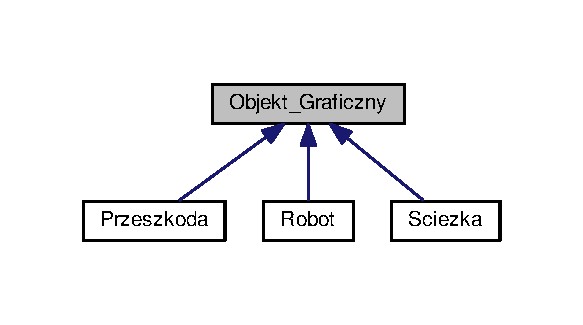
\includegraphics[width=280pt]{class_objekt___graficzny__inherit__graph}
\end{center}
\end{figure}
\subsection*{Public Member Functions}
\begin{DoxyCompactItemize}
\item 
\hypertarget{class_objekt___graficzny_a77cf5352485959ba5b511e6241080e1c}{\hyperlink{class_objekt___graficzny_a77cf5352485959ba5b511e6241080e1c}{Objekt\+\_\+\+Graficzny} ()}\label{class_objekt___graficzny_a77cf5352485959ba5b511e6241080e1c}

\begin{DoxyCompactList}\small\item\em Inicjalizacja Obiektu graficznego. \end{DoxyCompactList}\item 
\hyperlink{class_objekt___graficzny_a78795f7fdc63bcfa813dccafe689dbad}{Objekt\+\_\+\+Graficzny} (std\+::vector$<$ double $>$ Wspolrzedne\+\_\+\+Wierzcholkow, const double \&Kat\+\_\+\+Obrotu)
\begin{DoxyCompactList}\small\item\em Inicjalizacja zmiennej typu \hyperlink{class_zbior_wierzcholkow}{Zbior\+Wierzcholkow} wartosciami. \end{DoxyCompactList}\item 
\hyperlink{class_objekt___graficzny_a02028426a39d3b8be08b183adbf291c3}{Objekt\+\_\+\+Graficzny} (std\+::vector$<$ \hyperlink{class_wektor2_d}{Wektor2\+D} $>$ Wierzcholki, const double \&Kat\+\_\+\+Obrotu)
\begin{DoxyCompactList}\small\item\em Inicjalizacja zmiennej typu \hyperlink{class_zbior_wierzcholkow}{Zbior\+Wierzcholkow} wartosciami. \end{DoxyCompactList}\item 
\hyperlink{class_objekt___graficzny_aafb4740ff40c5719ff2da044a0797d2b}{Objekt\+\_\+\+Graficzny} (std\+::vector$<$ double $>$ Wspolrzedne\+\_\+\+Wierzcholkow, const \hyperlink{class_wektor2_d}{Wektor2\+D} \&Wspolrzedne\+\_\+\+Globalne, const double \&Kat\+\_\+\+Obrotu)
\begin{DoxyCompactList}\small\item\em Inicjalizacja zmiennej typu \hyperlink{class_zbior_wierzcholkow}{Zbior\+Wierzcholkow} wartosciami. \end{DoxyCompactList}\item 
\hyperlink{class_objekt___graficzny_a116ad8942cd4217c5eb288e4a21dce20}{Objekt\+\_\+\+Graficzny} (std\+::vector$<$ \hyperlink{class_wektor2_d}{Wektor2\+D} $>$ Wierzcholki, const \hyperlink{class_wektor2_d}{Wektor2\+D} \&Wspolrzedne\+\_\+\+Globalne, const double \&Kat\+\_\+\+Obrotu)
\begin{DoxyCompactList}\small\item\em Inicjalizacja zmiennej typu \hyperlink{class_zbior_wierzcholkow}{Zbior\+Wierzcholkow} wartosciami. \end{DoxyCompactList}\item 
\hypertarget{class_objekt___graficzny_a23eda6cc50a9926ff066e01cf2728af8}{int \hyperlink{class_objekt___graficzny_a23eda6cc50a9926ff066e01cf2728af8}{Rozmiar} () const }\label{class_objekt___graficzny_a23eda6cc50a9926ff066e01cf2728af8}

\begin{DoxyCompactList}\small\item\em Zwraca liczbę istniejących wierzchołków. \end{DoxyCompactList}\item 
\hypertarget{class_objekt___graficzny_ac2df01dee82aa90b651f6c0f24d25796}{double \hyperlink{class_objekt___graficzny_ac2df01dee82aa90b651f6c0f24d25796}{Kat} () const }\label{class_objekt___graficzny_ac2df01dee82aa90b651f6c0f24d25796}

\begin{DoxyCompactList}\small\item\em Zwraca ustawiony kąt obrotu. \end{DoxyCompactList}\item 
\hypertarget{class_objekt___graficzny_ae2da90c757c1b9052dd8ffa692a09caf}{void \hyperlink{class_objekt___graficzny_ae2da90c757c1b9052dd8ffa692a09caf}{Kat} (const double \&Kat\+\_\+\+Obrotu)}\label{class_objekt___graficzny_ae2da90c757c1b9052dd8ffa692a09caf}

\begin{DoxyCompactList}\small\item\em Ustawia kąt obrotu. \end{DoxyCompactList}\item 
void \hyperlink{class_objekt___graficzny_a8696af86777439596367520e67e824b9}{Ustaw} (std\+::vector$<$ double $>$ Wspolrzedne\+\_\+\+Wierzcholkow)
\begin{DoxyCompactList}\small\item\em Dodaje kolejne wierzchołki. \end{DoxyCompactList}\item 
void \hyperlink{class_objekt___graficzny_aa53a8a0cb8886e4aeb0b843d7bfff53a}{Ustaw} (\hyperlink{class_wektor2_d}{Wektor2\+D} Wierzcholek)
\begin{DoxyCompactList}\small\item\em Dodaje kolejne wierzchołki. \end{DoxyCompactList}\item 
void \hyperlink{class_objekt___graficzny_aea7b281802a335bc075a09a570538b5c}{Ustaw} (std\+::vector$<$ \hyperlink{class_wektor2_d}{Wektor2\+D} $>$ Wierzcholki)
\begin{DoxyCompactList}\small\item\em Dodaje kolejne wierzchołki. \end{DoxyCompactList}\item 
void \hyperlink{class_objekt___graficzny_aec73cbdb6b8e8519dd9f418a37072ae3}{Usun\+\_\+\+Elementy} (int Liczba\+\_\+elementow)
\begin{DoxyCompactList}\small\item\em Usuwa wybraną ilość elementów od końca. \end{DoxyCompactList}\item 
\hypertarget{class_objekt___graficzny_aa508473ea86c48f2d0acb5339f47177d}{void \hyperlink{class_objekt___graficzny_aa508473ea86c48f2d0acb5339f47177d}{Usun\+\_\+\+Elementy} ()}\label{class_objekt___graficzny_aa508473ea86c48f2d0acb5339f47177d}

\begin{DoxyCompactList}\small\item\em Usuwa wszystkie elementy. \end{DoxyCompactList}\item 
\hypertarget{class_objekt___graficzny_ad893e3051506b480a1338c2c234859d3}{\hyperlink{class_wektor2_d}{Wektor2\+D} \hyperlink{class_objekt___graficzny_ad893e3051506b480a1338c2c234859d3}{Wartosc\+\_\+\+Lok} (int Ind) const }\label{class_objekt___graficzny_ad893e3051506b480a1338c2c234859d3}

\begin{DoxyCompactList}\small\item\em Zwraca lokalne współrzędne wierzchołka Ind. \end{DoxyCompactList}\item 
void \hyperlink{class_objekt___graficzny_aca0acf1d25d7db81c40e9762a7f85072}{Wartosc\+\_\+\+Lok} (int Ind, const \hyperlink{class_wektor2_d}{Wektor2\+D} \&Wek)
\begin{DoxyCompactList}\small\item\em Ustawia lokalną wartosc wierzcholka nr Ind. \end{DoxyCompactList}\item 
\hypertarget{class_objekt___graficzny_a9872ecb81143f6f5a7e2296b354c0bcc}{\hyperlink{class_wektor2_d}{Wektor2\+D} \hyperlink{class_objekt___graficzny_a9872ecb81143f6f5a7e2296b354c0bcc}{Wartosc\+\_\+\+Glob} (int Ind) const }\label{class_objekt___graficzny_a9872ecb81143f6f5a7e2296b354c0bcc}

\begin{DoxyCompactList}\small\item\em Zwraca globalne współrzędne wierzchołka Ind. \end{DoxyCompactList}\item 
void \hyperlink{class_objekt___graficzny_afbe393725fafac38ac1dbf42486c1467}{Wartosc\+\_\+\+Glob} (int Ind, \hyperlink{class_wektor2_d}{Wektor2\+D} Wek)
\begin{DoxyCompactList}\small\item\em Ustawia globalne wartosc wierzcholka nr Ind. \end{DoxyCompactList}\item 
\hyperlink{class_wektor2_d}{Wektor2\+D} \hyperlink{class_objekt___graficzny_a14be7409a5989797c6197536d8f577d5}{operator\mbox{[}$\,$\mbox{]}} (int Ind) const 
\begin{DoxyCompactList}\small\item\em Przeciarzenie operatra indeksowania do zwracania wartosci. \end{DoxyCompactList}\item 
\hypertarget{class_objekt___graficzny_ae3e239a8ea20f6849d13c1eaf4a29b28}{void \hyperlink{class_objekt___graficzny_ae3e239a8ea20f6849d13c1eaf4a29b28}{Wyswietl} () const }\label{class_objekt___graficzny_ae3e239a8ea20f6849d13c1eaf4a29b28}

\begin{DoxyCompactList}\small\item\em Funkcja wypisuje do strumienia właściwości klasy. \end{DoxyCompactList}\item 
bool \hyperlink{class_objekt___graficzny_ac3028c59aa6332787b63e0f79fa69d52}{Koniec\+\_\+\+Animacji} ()
\begin{DoxyCompactList}\small\item\em Funkcja informuje czy nastąpił koniec animacji. \end{DoxyCompactList}\item 
void \hyperlink{class_objekt___graficzny_ae830af8c088c3f056a29b85eb62ca482}{Koniec\+\_\+\+Animacji} (bool Nastapil\+\_\+\+Koniec)
\begin{DoxyCompactList}\small\item\em Funkcja ustawia flagę końca animacji. \end{DoxyCompactList}\item 
virtual bool \hyperlink{class_objekt___graficzny_a90300b4487267d5a3ae0e4b8a6ab29bc}{Kolizja} ()
\begin{DoxyCompactList}\small\item\em Funkcja informuje czy nastąpiła kolizja. \end{DoxyCompactList}\item 
\hypertarget{class_objekt___graficzny_ac6c74e172b8d7b1af225d9d715aa2adb}{virtual void \hyperlink{class_objekt___graficzny_ac6c74e172b8d7b1af225d9d715aa2adb}{Wyswietl\+Wspolrzedne\+Format\+Gnuplot} (std\+::ostream \&Strm\+Wy) const }\label{class_objekt___graficzny_ac6c74e172b8d7b1af225d9d715aa2adb}

\begin{DoxyCompactList}\small\item\em Funkcja wypisuje do strumienia punkty w odpowiednim formacie. \end{DoxyCompactList}\item 
\hypertarget{class_objekt___graficzny_a4c6d923812b319e2907ec7a2db71feb1}{virtual \hyperlink{_objekt___graficzny_8hh_a59b4a471a7481f2a0551d90a8a745c9f}{Tryb\+\_\+\+Pracy} \hyperlink{class_objekt___graficzny_a4c6d923812b319e2907ec7a2db71feb1}{Rodzaj\+\_\+\+Obiektu} ()}\label{class_objekt___graficzny_a4c6d923812b319e2907ec7a2db71feb1}

\begin{DoxyCompactList}\small\item\em Zwraca tryb pracy w którym pracuje Obiekt\+\_\+\+Graficzny. \end{DoxyCompactList}\item 
\hypertarget{class_objekt___graficzny_a772090d97002afb5abcdbd6e1883e77b}{virtual std\+::string \hyperlink{class_objekt___graficzny_a772090d97002afb5abcdbd6e1883e77b}{Rodzaj\+\_\+\+Obiektu\+\_\+\+Nazwa} () const }\label{class_objekt___graficzny_a772090d97002afb5abcdbd6e1883e77b}

\begin{DoxyCompactList}\small\item\em Zwraca tryb pracy w którym pracuje Obiekt\+\_\+\+Graficzny. \end{DoxyCompactList}\end{DoxyCompactItemize}
\subsection*{Static Public Member Functions}
\begin{DoxyCompactItemize}
\item 
\hypertarget{class_objekt___graficzny_a3c2618724fff0c58433d50f811a166f5}{static void \hyperlink{class_objekt___graficzny_a3c2618724fff0c58433d50f811a166f5}{Wsp\+\_\+\+Glob} (const \hyperlink{class_wektor2_d}{Wektor2\+D} \&Wspolrzedne\+\_\+\+Globalne)}\label{class_objekt___graficzny_a3c2618724fff0c58433d50f811a166f5}

\begin{DoxyCompactList}\small\item\em Ustawia współrzędne globalne. \end{DoxyCompactList}\item 
\hypertarget{class_objekt___graficzny_ae2372551a897cab2b7ce0fadbb31ed5e}{static \hyperlink{class_wektor2_d}{Wektor2\+D} \hyperlink{class_objekt___graficzny_ae2372551a897cab2b7ce0fadbb31ed5e}{Wsp\+\_\+\+Glob} ()}\label{class_objekt___graficzny_ae2372551a897cab2b7ce0fadbb31ed5e}

\begin{DoxyCompactList}\small\item\em Ustawia współrzędne globalne. \end{DoxyCompactList}\end{DoxyCompactItemize}


\subsection{Detailed Description}
Modeluje informacje dotyczace \hyperlink{class_objekt___graficzny}{Objekt\+\_\+\+Graficzny}. 

Modeluje zestaw informacji dotyczacych wszystkich objektów występujących na scenie. Udostępnia także metody umozliwiające aktualizowanie wartosci a także zwracanie ich. 

\subsection{Constructor \& Destructor Documentation}
\hypertarget{class_objekt___graficzny_a78795f7fdc63bcfa813dccafe689dbad}{\index{Objekt\+\_\+\+Graficzny@{Objekt\+\_\+\+Graficzny}!Objekt\+\_\+\+Graficzny@{Objekt\+\_\+\+Graficzny}}
\index{Objekt\+\_\+\+Graficzny@{Objekt\+\_\+\+Graficzny}!Objekt\+\_\+\+Graficzny@{Objekt\+\_\+\+Graficzny}}
\subsubsection[{Objekt\+\_\+\+Graficzny}]{\setlength{\rightskip}{0pt plus 5cm}Objekt\+\_\+\+Graficzny\+::\+Objekt\+\_\+\+Graficzny (
\begin{DoxyParamCaption}
\item[{std\+::vector$<$ double $>$}]{Wspolrzedne\+\_\+\+Wierzcholkow, }
\item[{const double \&}]{Kat\+\_\+\+Obrotu}
\end{DoxyParamCaption}
)\hspace{0.3cm}{\ttfamily [inline]}}}\label{class_objekt___graficzny_a78795f7fdc63bcfa813dccafe689dbad}


Inicjalizacja zmiennej typu \hyperlink{class_zbior_wierzcholkow}{Zbior\+Wierzcholkow} wartosciami. 


\begin{DoxyParams}[1]{Parameters}
\mbox{\tt in}  & {\em Wspolrzedne\+\_\+\+Wierzcholkow} & ustawia parametry wspolrzednych wierzcholkow. Należy podać je w kolejności\+: Wsp\+X\+\_\+\+Wierzch1 Wsp\+Y\+\_\+\+Wierzch1 Wsp\+X\+\_\+\+Wierzch2 ... \\
\hline
\mbox{\tt in}  & {\em Kat\+\_\+\+Obrotu} & Kąt obrotu o jaki obrócić wierzchołki względem domyślego położenia \\
\hline
\end{DoxyParams}
\hypertarget{class_objekt___graficzny_a02028426a39d3b8be08b183adbf291c3}{\index{Objekt\+\_\+\+Graficzny@{Objekt\+\_\+\+Graficzny}!Objekt\+\_\+\+Graficzny@{Objekt\+\_\+\+Graficzny}}
\index{Objekt\+\_\+\+Graficzny@{Objekt\+\_\+\+Graficzny}!Objekt\+\_\+\+Graficzny@{Objekt\+\_\+\+Graficzny}}
\subsubsection[{Objekt\+\_\+\+Graficzny}]{\setlength{\rightskip}{0pt plus 5cm}Objekt\+\_\+\+Graficzny\+::\+Objekt\+\_\+\+Graficzny (
\begin{DoxyParamCaption}
\item[{std\+::vector$<$ {\bf Wektor2\+D} $>$}]{Wierzcholki, }
\item[{const double \&}]{Kat\+\_\+\+Obrotu}
\end{DoxyParamCaption}
)\hspace{0.3cm}{\ttfamily [inline]}}}\label{class_objekt___graficzny_a02028426a39d3b8be08b183adbf291c3}


Inicjalizacja zmiennej typu \hyperlink{class_zbior_wierzcholkow}{Zbior\+Wierzcholkow} wartosciami. 

Każdy wierzchołek jest oreślony jako wektor


\begin{DoxyParams}[1]{Parameters}
\mbox{\tt in}  & {\em Wierzcholki} & ustawia parametry wspolrzednych wierzcholkow. \\
\hline
\mbox{\tt in}  & {\em Kat\+\_\+\+Obrotu} & Kąt obrotu o jaki obrócić wierzchołki względem domyślego położenia \\
\hline
\end{DoxyParams}
\hypertarget{class_objekt___graficzny_aafb4740ff40c5719ff2da044a0797d2b}{\index{Objekt\+\_\+\+Graficzny@{Objekt\+\_\+\+Graficzny}!Objekt\+\_\+\+Graficzny@{Objekt\+\_\+\+Graficzny}}
\index{Objekt\+\_\+\+Graficzny@{Objekt\+\_\+\+Graficzny}!Objekt\+\_\+\+Graficzny@{Objekt\+\_\+\+Graficzny}}
\subsubsection[{Objekt\+\_\+\+Graficzny}]{\setlength{\rightskip}{0pt plus 5cm}Objekt\+\_\+\+Graficzny\+::\+Objekt\+\_\+\+Graficzny (
\begin{DoxyParamCaption}
\item[{std\+::vector$<$ double $>$}]{Wspolrzedne\+\_\+\+Wierzcholkow, }
\item[{const {\bf Wektor2\+D} \&}]{Wspolrzedne\+\_\+\+Globalne, }
\item[{const double \&}]{Kat\+\_\+\+Obrotu}
\end{DoxyParamCaption}
)\hspace{0.3cm}{\ttfamily [inline]}}}\label{class_objekt___graficzny_aafb4740ff40c5719ff2da044a0797d2b}


Inicjalizacja zmiennej typu \hyperlink{class_zbior_wierzcholkow}{Zbior\+Wierzcholkow} wartosciami. 


\begin{DoxyParams}[1]{Parameters}
\mbox{\tt in}  & {\em Wspolrzedne\+\_\+\+Wierzcholkow} & ustawia parametry wspolrzednych wierzcholkow. Należy podać je w kolejności\+: Wsp\+X\+\_\+\+Wierzch1 Wsp\+Y\+\_\+\+Wierzch1 Wsp\+X\+\_\+\+Wierzch2 ... \\
\hline
\mbox{\tt in}  & {\em Wspolrzedne\+\_\+\+Globalne} & Współrzędne globalne \\
\hline
\mbox{\tt in}  & {\em Kat\+\_\+\+Obrotu} & Kąt obrotu o jaki obrócić wierzchołki względem domyślego położenia \\
\hline
\end{DoxyParams}
\hypertarget{class_objekt___graficzny_a116ad8942cd4217c5eb288e4a21dce20}{\index{Objekt\+\_\+\+Graficzny@{Objekt\+\_\+\+Graficzny}!Objekt\+\_\+\+Graficzny@{Objekt\+\_\+\+Graficzny}}
\index{Objekt\+\_\+\+Graficzny@{Objekt\+\_\+\+Graficzny}!Objekt\+\_\+\+Graficzny@{Objekt\+\_\+\+Graficzny}}
\subsubsection[{Objekt\+\_\+\+Graficzny}]{\setlength{\rightskip}{0pt plus 5cm}Objekt\+\_\+\+Graficzny\+::\+Objekt\+\_\+\+Graficzny (
\begin{DoxyParamCaption}
\item[{std\+::vector$<$ {\bf Wektor2\+D} $>$}]{Wierzcholki, }
\item[{const {\bf Wektor2\+D} \&}]{Wspolrzedne\+\_\+\+Globalne, }
\item[{const double \&}]{Kat\+\_\+\+Obrotu}
\end{DoxyParamCaption}
)\hspace{0.3cm}{\ttfamily [inline]}}}\label{class_objekt___graficzny_a116ad8942cd4217c5eb288e4a21dce20}


Inicjalizacja zmiennej typu \hyperlink{class_zbior_wierzcholkow}{Zbior\+Wierzcholkow} wartosciami. 

Każdy wierzchołek jest oreślony jako wektor


\begin{DoxyParams}[1]{Parameters}
\mbox{\tt in}  & {\em Wierzcholki} & ustawia parametry wspolrzednych wierzcholkow. \\
\hline
\mbox{\tt in}  & {\em Wspolrzedne\+\_\+\+Globalne} & Współrzędne globalne \\
\hline
\mbox{\tt in}  & {\em Kat\+\_\+\+Obrotu} & Kąt obrotu o jaki obrócić wierzchołki względem domyślego położenia \\
\hline
\end{DoxyParams}


\subsection{Member Function Documentation}
\hypertarget{class_objekt___graficzny_a90300b4487267d5a3ae0e4b8a6ab29bc}{\index{Objekt\+\_\+\+Graficzny@{Objekt\+\_\+\+Graficzny}!Kolizja@{Kolizja}}
\index{Kolizja@{Kolizja}!Objekt\+\_\+\+Graficzny@{Objekt\+\_\+\+Graficzny}}
\subsubsection[{Kolizja}]{\setlength{\rightskip}{0pt plus 5cm}virtual bool Objekt\+\_\+\+Graficzny\+::\+Kolizja (
\begin{DoxyParamCaption}
{}
\end{DoxyParamCaption}
)\hspace{0.3cm}{\ttfamily [inline]}, {\ttfamily [virtual]}}}\label{class_objekt___graficzny_a90300b4487267d5a3ae0e4b8a6ab29bc}


Funkcja informuje czy nastąpiła kolizja. 


\begin{DoxyRetVals}{Return values}
{\em true} & -\/ Jeżeli nastąpiła kolizja \\
\hline
{\em false} & -\/ Jeżeli nie nastąpiła kolizja \\
\hline
\end{DoxyRetVals}
\hypertarget{class_objekt___graficzny_ac3028c59aa6332787b63e0f79fa69d52}{\index{Objekt\+\_\+\+Graficzny@{Objekt\+\_\+\+Graficzny}!Koniec\+\_\+\+Animacji@{Koniec\+\_\+\+Animacji}}
\index{Koniec\+\_\+\+Animacji@{Koniec\+\_\+\+Animacji}!Objekt\+\_\+\+Graficzny@{Objekt\+\_\+\+Graficzny}}
\subsubsection[{Koniec\+\_\+\+Animacji}]{\setlength{\rightskip}{0pt plus 5cm}bool Objekt\+\_\+\+Graficzny\+::\+Koniec\+\_\+\+Animacji (
\begin{DoxyParamCaption}
{}
\end{DoxyParamCaption}
)\hspace{0.3cm}{\ttfamily [inline]}}}\label{class_objekt___graficzny_ac3028c59aa6332787b63e0f79fa69d52}


Funkcja informuje czy nastąpił koniec animacji. 


\begin{DoxyRetVals}{Return values}
{\em true} & -\/ Jeżeli nastąpił koniec animacji \\
\hline
{\em false} & -\/ Jeżeli jeszcze nie nastąpił koniec animacji \\
\hline
\end{DoxyRetVals}
\hypertarget{class_objekt___graficzny_ae830af8c088c3f056a29b85eb62ca482}{\index{Objekt\+\_\+\+Graficzny@{Objekt\+\_\+\+Graficzny}!Koniec\+\_\+\+Animacji@{Koniec\+\_\+\+Animacji}}
\index{Koniec\+\_\+\+Animacji@{Koniec\+\_\+\+Animacji}!Objekt\+\_\+\+Graficzny@{Objekt\+\_\+\+Graficzny}}
\subsubsection[{Koniec\+\_\+\+Animacji}]{\setlength{\rightskip}{0pt plus 5cm}void Objekt\+\_\+\+Graficzny\+::\+Koniec\+\_\+\+Animacji (
\begin{DoxyParamCaption}
\item[{bool}]{Nastapil\+\_\+\+Koniec}
\end{DoxyParamCaption}
)\hspace{0.3cm}{\ttfamily [inline]}}}\label{class_objekt___graficzny_ae830af8c088c3f056a29b85eb62ca482}


Funkcja ustawia flagę końca animacji. 


\begin{DoxyRetVals}{Return values}
{\em true} & -\/ Jeżeli nastąpił koniec animacji \\
\hline
{\em false} & -\/ Jeżeli jeszcze nie nastąpił koniec animacji \\
\hline
\end{DoxyRetVals}
\hypertarget{class_objekt___graficzny_a14be7409a5989797c6197536d8f577d5}{\index{Objekt\+\_\+\+Graficzny@{Objekt\+\_\+\+Graficzny}!operator\mbox{[}$\,$\mbox{]}@{operator[]}}
\index{operator\mbox{[}$\,$\mbox{]}@{operator[]}!Objekt\+\_\+\+Graficzny@{Objekt\+\_\+\+Graficzny}}
\subsubsection[{operator[]}]{\setlength{\rightskip}{0pt plus 5cm}{\bf Wektor2\+D} Objekt\+\_\+\+Graficzny\+::operator\mbox{[}$\,$\mbox{]} (
\begin{DoxyParamCaption}
\item[{int}]{Ind}
\end{DoxyParamCaption}
) const\hspace{0.3cm}{\ttfamily [inline]}}}\label{class_objekt___graficzny_a14be7409a5989797c6197536d8f577d5}


Przeciarzenie operatra indeksowania do zwracania wartosci. 

Wartość zwracana z uwzględnieniem położenia globalnego \hypertarget{class_objekt___graficzny_a8696af86777439596367520e67e824b9}{\index{Objekt\+\_\+\+Graficzny@{Objekt\+\_\+\+Graficzny}!Ustaw@{Ustaw}}
\index{Ustaw@{Ustaw}!Objekt\+\_\+\+Graficzny@{Objekt\+\_\+\+Graficzny}}
\subsubsection[{Ustaw}]{\setlength{\rightskip}{0pt plus 5cm}void Objekt\+\_\+\+Graficzny\+::\+Ustaw (
\begin{DoxyParamCaption}
\item[{std\+::vector$<$ double $>$}]{Wspolrzedne\+\_\+\+Wierzcholkow}
\end{DoxyParamCaption}
)\hspace{0.3cm}{\ttfamily [inline]}}}\label{class_objekt___graficzny_a8696af86777439596367520e67e824b9}


Dodaje kolejne wierzchołki. 


\begin{DoxyParams}[1]{Parameters}
\mbox{\tt in}  & {\em Wspolrzedne\+\_\+\+Wierzcholkow} & ustawia parametry wspolrzednych wierzcholkow. Należy podać je w kolejności\+: Wsp\+X\+\_\+\+Wierzch1 Wsp\+Y\+\_\+\+Wierzch1 Wsp\+X\+\_\+\+Wierzch2 ... \\
\hline
\end{DoxyParams}
\hypertarget{class_objekt___graficzny_aa53a8a0cb8886e4aeb0b843d7bfff53a}{\index{Objekt\+\_\+\+Graficzny@{Objekt\+\_\+\+Graficzny}!Ustaw@{Ustaw}}
\index{Ustaw@{Ustaw}!Objekt\+\_\+\+Graficzny@{Objekt\+\_\+\+Graficzny}}
\subsubsection[{Ustaw}]{\setlength{\rightskip}{0pt plus 5cm}void Objekt\+\_\+\+Graficzny\+::\+Ustaw (
\begin{DoxyParamCaption}
\item[{{\bf Wektor2\+D}}]{Wierzcholek}
\end{DoxyParamCaption}
)\hspace{0.3cm}{\ttfamily [inline]}}}\label{class_objekt___graficzny_aa53a8a0cb8886e4aeb0b843d7bfff53a}


Dodaje kolejne wierzchołki. 


\begin{DoxyParams}[1]{Parameters}
\mbox{\tt in}  & {\em Wierzcholek} & Wierzchołek, który ma być dodany na koniec powinien być typu \hyperlink{class_wektor2_d}{Wektor2\+D} \\
\hline
\end{DoxyParams}
\hypertarget{class_objekt___graficzny_aea7b281802a335bc075a09a570538b5c}{\index{Objekt\+\_\+\+Graficzny@{Objekt\+\_\+\+Graficzny}!Ustaw@{Ustaw}}
\index{Ustaw@{Ustaw}!Objekt\+\_\+\+Graficzny@{Objekt\+\_\+\+Graficzny}}
\subsubsection[{Ustaw}]{\setlength{\rightskip}{0pt plus 5cm}void Objekt\+\_\+\+Graficzny\+::\+Ustaw (
\begin{DoxyParamCaption}
\item[{std\+::vector$<$ {\bf Wektor2\+D} $>$}]{Wierzcholki}
\end{DoxyParamCaption}
)\hspace{0.3cm}{\ttfamily [inline]}}}\label{class_objekt___graficzny_aea7b281802a335bc075a09a570538b5c}


Dodaje kolejne wierzchołki. 


\begin{DoxyParams}[1]{Parameters}
\mbox{\tt in}  & {\em Wierzcholki} & Wierzchołki, które mają być kolejno dodane powinny być typu \hyperlink{class_wektor2_d}{Wektor2\+D} \\
\hline
\end{DoxyParams}
\hypertarget{class_objekt___graficzny_aec73cbdb6b8e8519dd9f418a37072ae3}{\index{Objekt\+\_\+\+Graficzny@{Objekt\+\_\+\+Graficzny}!Usun\+\_\+\+Elementy@{Usun\+\_\+\+Elementy}}
\index{Usun\+\_\+\+Elementy@{Usun\+\_\+\+Elementy}!Objekt\+\_\+\+Graficzny@{Objekt\+\_\+\+Graficzny}}
\subsubsection[{Usun\+\_\+\+Elementy}]{\setlength{\rightskip}{0pt plus 5cm}void Objekt\+\_\+\+Graficzny\+::\+Usun\+\_\+\+Elementy (
\begin{DoxyParamCaption}
\item[{int}]{Liczba\+\_\+elementow}
\end{DoxyParamCaption}
)\hspace{0.3cm}{\ttfamily [inline]}}}\label{class_objekt___graficzny_aec73cbdb6b8e8519dd9f418a37072ae3}


Usuwa wybraną ilość elementów od końca. 


\begin{DoxyParams}[1]{Parameters}
\mbox{\tt in}  & {\em Liczba\+\_\+elementow} & Ile ostatnich elementów usunąć \\
\hline
\end{DoxyParams}
\hypertarget{class_objekt___graficzny_afbe393725fafac38ac1dbf42486c1467}{\index{Objekt\+\_\+\+Graficzny@{Objekt\+\_\+\+Graficzny}!Wartosc\+\_\+\+Glob@{Wartosc\+\_\+\+Glob}}
\index{Wartosc\+\_\+\+Glob@{Wartosc\+\_\+\+Glob}!Objekt\+\_\+\+Graficzny@{Objekt\+\_\+\+Graficzny}}
\subsubsection[{Wartosc\+\_\+\+Glob}]{\setlength{\rightskip}{0pt plus 5cm}void Objekt\+\_\+\+Graficzny\+::\+Wartosc\+\_\+\+Glob (
\begin{DoxyParamCaption}
\item[{int}]{Ind, }
\item[{{\bf Wektor2\+D}}]{Wek}
\end{DoxyParamCaption}
)\hspace{0.3cm}{\ttfamily [inline]}}}\label{class_objekt___graficzny_afbe393725fafac38ac1dbf42486c1467}


Ustawia globalne wartosc wierzcholka nr Ind. 


\begin{DoxyParams}[1]{Parameters}
\mbox{\tt in}  & {\em Ind} & Wierzchołek, którego wartość ma być zmieniona \\
\hline
\mbox{\tt in}  & {\em Wek} & Wektor na jaki ma być zmieniony wierzchołek \\
\hline
\end{DoxyParams}
\hypertarget{class_objekt___graficzny_aca0acf1d25d7db81c40e9762a7f85072}{\index{Objekt\+\_\+\+Graficzny@{Objekt\+\_\+\+Graficzny}!Wartosc\+\_\+\+Lok@{Wartosc\+\_\+\+Lok}}
\index{Wartosc\+\_\+\+Lok@{Wartosc\+\_\+\+Lok}!Objekt\+\_\+\+Graficzny@{Objekt\+\_\+\+Graficzny}}
\subsubsection[{Wartosc\+\_\+\+Lok}]{\setlength{\rightskip}{0pt plus 5cm}void Objekt\+\_\+\+Graficzny\+::\+Wartosc\+\_\+\+Lok (
\begin{DoxyParamCaption}
\item[{int}]{Ind, }
\item[{const {\bf Wektor2\+D} \&}]{Wek}
\end{DoxyParamCaption}
)\hspace{0.3cm}{\ttfamily [inline]}}}\label{class_objekt___graficzny_aca0acf1d25d7db81c40e9762a7f85072}


Ustawia lokalną wartosc wierzcholka nr Ind. 


\begin{DoxyParams}[1]{Parameters}
\mbox{\tt in}  & {\em Ind} & Wierzchołek, którego wartość ma być zmieniona \\
\hline
\mbox{\tt in}  & {\em Wek} & Wektor na jaki ma być zmieniony wierzchołek \\
\hline
\end{DoxyParams}


The documentation for this class was generated from the following files\+:\begin{DoxyCompactItemize}
\item 
/home/kstefanc/\+P\+O/\+Lab07/\+Lab/prj/inc/\hyperlink{_objekt___graficzny_8hh}{Objekt\+\_\+\+Graficzny.\+hh}\item 
/home/kstefanc/\+P\+O/\+Lab07/\+Lab/prj/src/main.\+cpp\item 
/home/kstefanc/\+P\+O/\+Lab07/\+Lab/prj/src/Objekt\+\_\+\+Graficzny.\+cpp\end{DoxyCompactItemize}

\hypertarget{class_robot}{\section{Robot Class Reference}
\label{class_robot}\index{Robot@{Robot}}
}


Modeluje informacje dotyczace prostokąta.  




{\ttfamily \#include $<$Robot.\+hh$>$}

\subsection*{Public Member Functions}
\begin{DoxyCompactItemize}
\item 
\hypertarget{class_robot_a4fc7c70ae20623f05e06f2ecb388b6c4}{\hyperlink{class_robot_a4fc7c70ae20623f05e06f2ecb388b6c4}{Robot} ()}\label{class_robot_a4fc7c70ae20623f05e06f2ecb388b6c4}

\begin{DoxyCompactList}\small\item\em Inicjalizacja Robota w pozycji podstawowej. \end{DoxyCompactList}\item 
\hypertarget{class_robot_a57616442d2907ac8a7e4e124d82b5ba3}{\hyperlink{class_robot_a57616442d2907ac8a7e4e124d82b5ba3}{Robot} (\hyperlink{class_wektor2_d}{Wektor2\+D} Wsp\+\_\+globalne)}\label{class_robot_a57616442d2907ac8a7e4e124d82b5ba3}

\begin{DoxyCompactList}\small\item\em Inicjalizacja Robota w pozycji podstawowej. \end{DoxyCompactList}\item 
\hypertarget{class_robot_aef89d67c7b58e5deb3a734fc816b800c}{\hyperlink{class_wektor2_d}{Wektor2\+D} \hyperlink{class_robot_aef89d67c7b58e5deb3a734fc816b800c}{Wartosc} (int Ind) const }\label{class_robot_aef89d67c7b58e5deb3a734fc816b800c}

\begin{DoxyCompactList}\small\item\em Zwraca współrzędne wierzchołka Ind. \end{DoxyCompactList}\item 
\hypertarget{class_robot_a3ec5e3a2db5fe429c765ed0a0d418eb8}{double \hyperlink{class_robot_a3ec5e3a2db5fe429c765ed0a0d418eb8}{Kat\+\_\+\+Obrotu} () const }\label{class_robot_a3ec5e3a2db5fe429c765ed0a0d418eb8}

\begin{DoxyCompactList}\small\item\em Zwraca kąt obrotu Robora. \end{DoxyCompactList}\item 
\hypertarget{class_robot_a327dff2175436c0be586e17c12bd9969}{\hyperlink{class_wektor2_d}{Wektor2\+D} \hyperlink{class_robot_a327dff2175436c0be586e17c12bd9969}{Wsp\+\_\+\+Globalne} () const }\label{class_robot_a327dff2175436c0be586e17c12bd9969}

\begin{DoxyCompactList}\small\item\em Zwraca współrzędne globalne robota. \end{DoxyCompactList}\item 
\hypertarget{class_robot_a1ad31789d90f6af2b3d512359e2e8421}{void \hyperlink{class_robot_a1ad31789d90f6af2b3d512359e2e8421}{Ustaw\+\_\+\+Wsp\+\_\+\+Globalne} (\hyperlink{class_wektor2_d}{Wektor2\+D} \hyperlink{class_robot_a327dff2175436c0be586e17c12bd9969}{Wsp\+\_\+\+Globalne})}\label{class_robot_a1ad31789d90f6af2b3d512359e2e8421}

\begin{DoxyCompactList}\small\item\em Ustawia współrzędne globalne robota. \end{DoxyCompactList}\item 
void \hyperlink{class_robot_a4d5ca83fe9dee72eddd8c6df97a0e10d}{Obroc\+O\+Kat} (double a)
\begin{DoxyCompactList}\small\item\em Obraca prostakat o kat a. \end{DoxyCompactList}\item 
bool \hyperlink{class_robot_a8e9a1014f600141e9a9514d6622b3394}{Zapis\+Wspolrzednych\+Do\+Pliku\+Format\+Gnuplot} (const char $\ast$s\+Nazwa\+Pliku)
\begin{DoxyCompactList}\small\item\em Zapisuje wspolrzedne do pliku w formacie zgodnym z Gnuplotem. \end{DoxyCompactList}\item 
\hypertarget{class_robot_a1a73604f8395ef66e6bf1e470108a77e}{void \hyperlink{class_robot_a1a73604f8395ef66e6bf1e470108a77e}{Wyswietl\+Wspolrzedne\+Format\+Gnuplot} (std\+::ostream \&Strm\+Wy) const }\label{class_robot_a1a73604f8395ef66e6bf1e470108a77e}

\begin{DoxyCompactList}\small\item\em Funkcja wypisuje do strumienia punkty w odpowiednim formacie. \end{DoxyCompactList}\item 
\hypertarget{class_robot_acd7c1bebb006bce05ae347e93d535f55}{\hyperlink{class_wektor2_d}{Wektor2\+D} \hyperlink{class_robot_acd7c1bebb006bce05ae347e93d535f55}{operator\mbox{[}$\,$\mbox{]}} (int Ind) const }\label{class_robot_acd7c1bebb006bce05ae347e93d535f55}

\begin{DoxyCompactList}\small\item\em Przeciarzenie operatra indeksowania do zwracania wartosci. \end{DoxyCompactList}\item 
\hypertarget{class_robot_af268b1aec21d67bf663f141163c05f9e}{\hyperlink{class_wektor2_d}{Wektor2\+D} \& \hyperlink{class_robot_af268b1aec21d67bf663f141163c05f9e}{operator\mbox{[}$\,$\mbox{]}} (int Ind)}\label{class_robot_af268b1aec21d67bf663f141163c05f9e}

\begin{DoxyCompactList}\small\item\em Przeciarzenie operatra indeksowania do przypisania wartosci. \end{DoxyCompactList}\end{DoxyCompactItemize}


\subsection{Detailed Description}
Modeluje informacje dotyczace prostokąta. 

Modeluje zestaw informacji dotyczacych prostokąta. Udostępnia także metody umozliwiające aktualizowanie wartosci a także zwracanie ich. 

\subsection{Member Function Documentation}
\hypertarget{class_robot_a4d5ca83fe9dee72eddd8c6df97a0e10d}{\index{Robot@{Robot}!Obroc\+O\+Kat@{Obroc\+O\+Kat}}
\index{Obroc\+O\+Kat@{Obroc\+O\+Kat}!Robot@{Robot}}
\subsubsection[{Obroc\+O\+Kat}]{\setlength{\rightskip}{0pt plus 5cm}void Robot\+::\+Obroc\+O\+Kat (
\begin{DoxyParamCaption}
\item[{double}]{a}
\end{DoxyParamCaption}
)}}\label{class_robot_a4d5ca83fe9dee72eddd8c6df97a0e10d}


Obraca prostakat o kat a. 


\begin{DoxyParams}[1]{Parameters}
\mbox{\tt in}  & {\em a} & kąt o jaki obrócić prostokąt \\
\hline
\end{DoxyParams}
\hypertarget{class_robot_a8e9a1014f600141e9a9514d6622b3394}{\index{Robot@{Robot}!Zapis\+Wspolrzednych\+Do\+Pliku\+Format\+Gnuplot@{Zapis\+Wspolrzednych\+Do\+Pliku\+Format\+Gnuplot}}
\index{Zapis\+Wspolrzednych\+Do\+Pliku\+Format\+Gnuplot@{Zapis\+Wspolrzednych\+Do\+Pliku\+Format\+Gnuplot}!Robot@{Robot}}
\subsubsection[{Zapis\+Wspolrzednych\+Do\+Pliku\+Format\+Gnuplot}]{\setlength{\rightskip}{0pt plus 5cm}bool Robot\+::\+Zapis\+Wspolrzednych\+Do\+Pliku\+Format\+Gnuplot (
\begin{DoxyParamCaption}
\item[{const char $\ast$}]{s\+Nazwa\+Pliku}
\end{DoxyParamCaption}
)}}\label{class_robot_a8e9a1014f600141e9a9514d6622b3394}


Zapisuje wspolrzedne do pliku w formacie zgodnym z Gnuplotem. 

Funkcja jest niewielką modyfikacją funkcji \char`\"{}\+Przyklad\+Zapisu\+Wspolrzednych\+Do\+Pliku\char`\"{} z pliku main dostarczonego w folderze zalazek 

The documentation for this class was generated from the following files\+:\begin{DoxyCompactItemize}
\item 
/home/kstefanc/\+P\+O/\+Lab06/\+Przygotowanie/prj/inc/\hyperlink{_robot_8hh}{Robot.\+hh}\item 
/home/kstefanc/\+P\+O/\+Lab06/\+Przygotowanie/prj/src/Robot.\+cpp\end{DoxyCompactItemize}

\hypertarget{class_scena}{\section{Scena Class Reference}
\label{class_scena}\index{Scena@{Scena}}
}


Modeluje informacje dotyczace Sceny.  




{\ttfamily \#include $<$Scena.\+hh$>$}



Collaboration diagram for Scena\+:\nopagebreak
\begin{figure}[H]
\begin{center}
\leavevmode
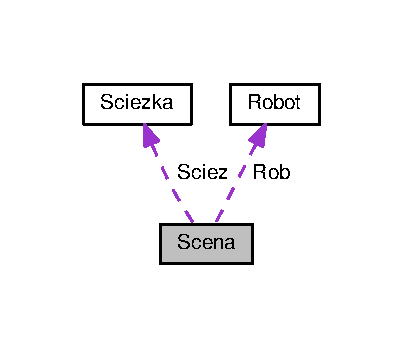
\includegraphics[width=194pt]{class_scena__coll__graph}
\end{center}
\end{figure}
\subsection*{Public Member Functions}
\begin{DoxyCompactItemize}
\item 
\hypertarget{class_scena_a8f9fe11b4cfef890123a2acc94672e17}{\hyperlink{class_scena_a8f9fe11b4cfef890123a2acc94672e17}{Scena} ()}\label{class_scena_a8f9fe11b4cfef890123a2acc94672e17}

\begin{DoxyCompactList}\small\item\em Funkcja odpowiada obliczenie punktu docelowego ruchu. \end{DoxyCompactList}\item 
bool \hyperlink{class_scena_a2a314381bd96a25eb210c2f62348205e}{Zapis\+Wspolrzednych\+Do\+Pliku\+Format\+Gnuplot} (const char $\ast$s\+Nazwa\+Pliku)
\begin{DoxyCompactList}\small\item\em Zapisuje wspolrzedne do pliku w formacie zgodnym z Gnuplotem. \end{DoxyCompactList}\item 
bool \hyperlink{class_scena_a04c424c45312771f98d823127282906e}{Animacja\+\_\+\+Sciezki\+\_\+\+Format\+Gnuplot} (\hyperlink{class_pz_g_1_1_lacze_do_g_n_u_plota}{Pz\+G\+::\+Lacze\+Do\+G\+N\+U\+Plota} Lacze, const char $\ast$s\+Nazwa\+Pliku, \hyperlink{class_sciezka}{Sciezka} Sciezka\+\_\+\+Animowana, \hyperlink{class_robot}{Robot} Robot\+\_\+\+Animowany, double dlugosc=0.\+25, int microseconds=40000)
\begin{DoxyCompactList}\small\item\em Animacja ścieżki wyświetlanej Gnuplotem. \end{DoxyCompactList}\item 
bool \hyperlink{class_scena_ac4a9a540d9a10739063568184892ad25}{Animacja\+\_\+\+Obrotu\+\_\+\+Format\+Gnuplot} (\hyperlink{class_pz_g_1_1_lacze_do_g_n_u_plota}{Pz\+G\+::\+Lacze\+Do\+G\+N\+U\+Plota} Lacze, const char $\ast$s\+Nazwa\+Pliku, \hyperlink{class_sciezka}{Sciezka} Sciezka\+\_\+\+Animowana, \hyperlink{class_robot}{Robot} Robot\+\_\+\+Animowany, int microseconds=40000, double a=1)
\begin{DoxyCompactList}\small\item\em Animacja obrotu robota wyświetlana Gnuplotem. \end{DoxyCompactList}\end{DoxyCompactItemize}
\subsection*{Public Attributes}
\begin{DoxyCompactItemize}
\item 
\hypertarget{class_scena_a349aabee5c459561924f0bf915cd8011}{\hyperlink{class_robot}{Robot} {\bfseries Rob}}\label{class_scena_a349aabee5c459561924f0bf915cd8011}

\item 
\hypertarget{class_scena_a0fb91d8e157e6c025a63b63f3b3f1115}{\hyperlink{class_sciezka}{Sciezka} {\bfseries Sciez}}\label{class_scena_a0fb91d8e157e6c025a63b63f3b3f1115}

\end{DoxyCompactItemize}


\subsection{Detailed Description}
Modeluje informacje dotyczace Sceny. 

Modeluje zestaw informacji dotyczacych wszystkich objektów występujących na scenie. Udostępnia także metody umozliwiające aktualizowanie wartosci a także zwracanie ich. 

\subsection{Member Function Documentation}
\hypertarget{class_scena_ac4a9a540d9a10739063568184892ad25}{\index{Scena@{Scena}!Animacja\+\_\+\+Obrotu\+\_\+\+Format\+Gnuplot@{Animacja\+\_\+\+Obrotu\+\_\+\+Format\+Gnuplot}}
\index{Animacja\+\_\+\+Obrotu\+\_\+\+Format\+Gnuplot@{Animacja\+\_\+\+Obrotu\+\_\+\+Format\+Gnuplot}!Scena@{Scena}}
\subsubsection[{Animacja\+\_\+\+Obrotu\+\_\+\+Format\+Gnuplot}]{\setlength{\rightskip}{0pt plus 5cm}bool Scena\+::\+Animacja\+\_\+\+Obrotu\+\_\+\+Format\+Gnuplot (
\begin{DoxyParamCaption}
\item[{{\bf Pz\+G\+::\+Lacze\+Do\+G\+N\+U\+Plota}}]{Lacze, }
\item[{const char $\ast$}]{s\+Nazwa\+Pliku, }
\item[{{\bf Sciezka}}]{Sciezka\+\_\+\+Animowana, }
\item[{{\bf Robot}}]{Robot\+\_\+\+Animowany, }
\item[{int}]{microseconds = {\ttfamily 40000}, }
\item[{double}]{a = {\ttfamily 1}}
\end{DoxyParamCaption}
)}}\label{class_scena_ac4a9a540d9a10739063568184892ad25}


Animacja obrotu robota wyświetlana Gnuplotem. 


\begin{DoxyParams}[1]{Parameters}
\mbox{\tt in}  & {\em s\+Nazwa\+Pliku} & -\/ Nazwa pliku do którego mają być wypisane wierzchołki \\
\hline
\mbox{\tt in}  & {\em Robot\+\_\+\+Animowany} & -\/ \hyperlink{class_robot}{Robot}, który ma być animowany wraz ze ścieżką \\
\hline
\mbox{\tt in}  & {\em microseconds} & -\/ długość trwania klatki w animacji \\
\hline
\mbox{\tt in}  & {\em a} & -\/ kąt kroku animacji \\
\hline
\end{DoxyParams}
\hypertarget{class_scena_a04c424c45312771f98d823127282906e}{\index{Scena@{Scena}!Animacja\+\_\+\+Sciezki\+\_\+\+Format\+Gnuplot@{Animacja\+\_\+\+Sciezki\+\_\+\+Format\+Gnuplot}}
\index{Animacja\+\_\+\+Sciezki\+\_\+\+Format\+Gnuplot@{Animacja\+\_\+\+Sciezki\+\_\+\+Format\+Gnuplot}!Scena@{Scena}}
\subsubsection[{Animacja\+\_\+\+Sciezki\+\_\+\+Format\+Gnuplot}]{\setlength{\rightskip}{0pt plus 5cm}bool Scena\+::\+Animacja\+\_\+\+Sciezki\+\_\+\+Format\+Gnuplot (
\begin{DoxyParamCaption}
\item[{{\bf Pz\+G\+::\+Lacze\+Do\+G\+N\+U\+Plota}}]{Lacze, }
\item[{const char $\ast$}]{s\+Nazwa\+Pliku, }
\item[{{\bf Sciezka}}]{Sciezka\+\_\+\+Animowana, }
\item[{{\bf Robot}}]{Robot\+\_\+\+Animowany, }
\item[{double}]{dlugosc = {\ttfamily 0.25}, }
\item[{int}]{microseconds = {\ttfamily 40000}}
\end{DoxyParamCaption}
)}}\label{class_scena_a04c424c45312771f98d823127282906e}


Animacja ścieżki wyświetlanej Gnuplotem. 


\begin{DoxyParams}[1]{Parameters}
\mbox{\tt in}  & {\em s\+Nazwa\+Pliku} & -\/ Nazwa pliku do którego mają być wypisane wierzchołki \\
\hline
\mbox{\tt in}  & {\em Robot\+\_\+\+Animowany} & -\/ \hyperlink{class_robot}{Robot}, który ma być animowany wraz ze ścieżką \\
\hline
\mbox{\tt in}  & {\em microseconds} & -\/ długość trwania klatki w animacji \\
\hline
\mbox{\tt in}  & {\em dlugosc} & -\/ długość kroku animacji \\
\hline
\end{DoxyParams}
\hypertarget{class_scena_a2a314381bd96a25eb210c2f62348205e}{\index{Scena@{Scena}!Zapis\+Wspolrzednych\+Do\+Pliku\+Format\+Gnuplot@{Zapis\+Wspolrzednych\+Do\+Pliku\+Format\+Gnuplot}}
\index{Zapis\+Wspolrzednych\+Do\+Pliku\+Format\+Gnuplot@{Zapis\+Wspolrzednych\+Do\+Pliku\+Format\+Gnuplot}!Scena@{Scena}}
\subsubsection[{Zapis\+Wspolrzednych\+Do\+Pliku\+Format\+Gnuplot}]{\setlength{\rightskip}{0pt plus 5cm}bool Scena\+::\+Zapis\+Wspolrzednych\+Do\+Pliku\+Format\+Gnuplot (
\begin{DoxyParamCaption}
\item[{const char $\ast$}]{s\+Nazwa\+Pliku}
\end{DoxyParamCaption}
)}}\label{class_scena_a2a314381bd96a25eb210c2f62348205e}


Zapisuje wspolrzedne do pliku w formacie zgodnym z Gnuplotem. 


\begin{DoxyParams}[1]{Parameters}
\mbox{\tt in}  & {\em s\+Nazwa\+Pliku} & -\/ Nazwa pliku do którego mają być wypisane wierzchołki \\
\hline
\end{DoxyParams}


The documentation for this class was generated from the following files\+:\begin{DoxyCompactItemize}
\item 
/home/kstefanc/\+P\+O/\+Lab06/\+Lab/prj/inc/\hyperlink{_scena_8hh}{Scena.\+hh}\item 
/home/kstefanc/\+P\+O/\+Lab06/\+Lab/prj/src/Scena.\+cpp\end{DoxyCompactItemize}

\hypertarget{class_sciezka}{\section{Sciezka Class Reference}
\label{class_sciezka}\index{Sciezka@{Sciezka}}
}


Modeluje informacje dotyczace Ścieżki.  




{\ttfamily \#include $<$Sciezka.\+hh$>$}



Inheritance diagram for Sciezka\+:\nopagebreak
\begin{figure}[H]
\begin{center}
\leavevmode
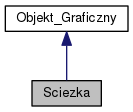
\includegraphics[width=172pt]{class_sciezka__inherit__graph}
\end{center}
\end{figure}


Collaboration diagram for Sciezka\+:\nopagebreak
\begin{figure}[H]
\begin{center}
\leavevmode
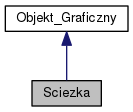
\includegraphics[width=172pt]{class_sciezka__coll__graph}
\end{center}
\end{figure}
\subsection*{Public Member Functions}
\begin{DoxyCompactItemize}
\item 
\hypertarget{class_sciezka_a95e9a0c51da72e4bd4edcca9f9ea7de4}{\hyperlink{class_sciezka_a95e9a0c51da72e4bd4edcca9f9ea7de4}{Sciezka} ()}\label{class_sciezka_a95e9a0c51da72e4bd4edcca9f9ea7de4}

\begin{DoxyCompactList}\small\item\em Funkcja odpowiada obliczenie punktu docelowego ruchu. \end{DoxyCompactList}\item 
\hyperlink{class_sciezka_a61da1d068b1b4cf437959dd4ec4f31b2}{Sciezka} (std\+::vector$<$ double $>$ Wspolrzedne\+\_\+\+Wierzcholkow, const \hyperlink{class_wektor2_d}{Wektor2\+D} \&Wspolrzedne\+\_\+\+Globalne, const double \&Kat\+\_\+\+Obrotu)
\begin{DoxyCompactList}\small\item\em Inicjalizacja zmiennej typu \hyperlink{class_zbior_wierzcholkow}{Zbior\+Wierzcholkow} wartosciami. \end{DoxyCompactList}\item 
\hyperlink{class_sciezka_ad33404b8f457cbd792fe746e639a0401}{Sciezka} (std\+::vector$<$ \hyperlink{class_wektor2_d}{Wektor2\+D} $>$ Wierzcholki, const \hyperlink{class_wektor2_d}{Wektor2\+D} \&Wspolrzedne\+\_\+\+Globalne, const double \&Kat\+\_\+\+Obrotu)
\begin{DoxyCompactList}\small\item\em Inicjalizacja zmiennej typu \hyperlink{class_zbior_wierzcholkow}{Zbior\+Wierzcholkow} wartosciami. \end{DoxyCompactList}\item 
void \hyperlink{class_sciezka_a37541491882dcd2e327f58207f376bd2}{Jedz\+\_\+\+Prosto} (\hyperlink{class_robot}{Robot} \&Rob, double dlugosc)
\begin{DoxyCompactList}\small\item\em Funkcja odpowiada obliczenie punktu docelowego ruchu. \end{DoxyCompactList}\item 
void \hyperlink{class_sciezka_a9fc6b8104ec42ffd5146fe4ca8ddd1ac}{Wyswietl\+Wspolrzedne\+Format\+Gnuplot} (std\+::ostream \&Strm\+Wy) const 
\begin{DoxyCompactList}\small\item\em Funkcja wypisuje punkty w formacie gnuplot. \end{DoxyCompactList}\item 
void \hyperlink{class_sciezka_a7d748699e2bf7940d76361b66b4fedba}{Przygotuj\+\_\+\+Animacje\+\_\+\+Sciezki} (\hyperlink{class_robot}{Robot} \&Rob, double dlugosc=1)
\begin{DoxyCompactList}\small\item\em Funkcja przygotowuje punkty pod animację \end{DoxyCompactList}\item 
void \hyperlink{class_sciezka_af673870927f8b8e88b1e31b8bb018de3}{Animacja\+\_\+\+Sciezki\+\_\+\+Z\+\_\+\+Robotem} (std\+::ostream \&Strm\+Wy, \hyperlink{class_robot}{Robot} \&Rob)
\begin{DoxyCompactList}\small\item\em Funkcja wypisuje kolejne punkty posrednie do strumienia tworząc animację robota i ścieżki. \end{DoxyCompactList}\item 
\hypertarget{class_sciezka_a3129be908dfd809c4c9339605e21e775}{double \hyperlink{class_sciezka_a3129be908dfd809c4c9339605e21e775}{Laczna\+\_\+\+Dlugosc\+\_\+\+Sciezki} ()}\label{class_sciezka_a3129be908dfd809c4c9339605e21e775}

\begin{DoxyCompactList}\small\item\em Funkcja zwraca łączną długość ścieżki. \end{DoxyCompactList}\end{DoxyCompactItemize}
\subsection*{Additional Inherited Members}


\subsection{Detailed Description}
Modeluje informacje dotyczace Ścieżki. 

Modeluje zestaw informacji dotyczacych ścieżki. Udostępnia także metody umozliwiające aktualizowanie wartosci a także zwracanie ich. 

\subsection{Constructor \& Destructor Documentation}
\hypertarget{class_sciezka_a61da1d068b1b4cf437959dd4ec4f31b2}{\index{Sciezka@{Sciezka}!Sciezka@{Sciezka}}
\index{Sciezka@{Sciezka}!Sciezka@{Sciezka}}
\subsubsection[{Sciezka}]{\setlength{\rightskip}{0pt plus 5cm}Sciezka\+::\+Sciezka (
\begin{DoxyParamCaption}
\item[{std\+::vector$<$ double $>$}]{Wspolrzedne\+\_\+\+Wierzcholkow, }
\item[{const {\bf Wektor2\+D} \&}]{Wspolrzedne\+\_\+\+Globalne, }
\item[{const double \&}]{Kat\+\_\+\+Obrotu}
\end{DoxyParamCaption}
)\hspace{0.3cm}{\ttfamily [inline]}}}\label{class_sciezka_a61da1d068b1b4cf437959dd4ec4f31b2}


Inicjalizacja zmiennej typu \hyperlink{class_zbior_wierzcholkow}{Zbior\+Wierzcholkow} wartosciami. 


\begin{DoxyParams}[1]{Parameters}
\mbox{\tt in}  & {\em Wspolrzedne\+\_\+\+Wierzcholkow} & ustawia parametry wspolrzednych wierzcholkow. Należy podać je w kolejności\+: Wsp\+X\+\_\+\+Wierzch1 Wsp\+Y\+\_\+\+Wierzch1 Wsp\+X\+\_\+\+Wierzch2 ... \\
\hline
\mbox{\tt in}  & {\em Wspolrzedne\+\_\+\+Globalne} & Współrzędne globalne \\
\hline
\mbox{\tt in}  & {\em Kat\+\_\+\+Obrotu} & Kąt obrotu o jaki obrócić wierzchołki względem domyślego położenia \\
\hline
\end{DoxyParams}
\hypertarget{class_sciezka_ad33404b8f457cbd792fe746e639a0401}{\index{Sciezka@{Sciezka}!Sciezka@{Sciezka}}
\index{Sciezka@{Sciezka}!Sciezka@{Sciezka}}
\subsubsection[{Sciezka}]{\setlength{\rightskip}{0pt plus 5cm}Sciezka\+::\+Sciezka (
\begin{DoxyParamCaption}
\item[{std\+::vector$<$ {\bf Wektor2\+D} $>$}]{Wierzcholki, }
\item[{const {\bf Wektor2\+D} \&}]{Wspolrzedne\+\_\+\+Globalne, }
\item[{const double \&}]{Kat\+\_\+\+Obrotu}
\end{DoxyParamCaption}
)\hspace{0.3cm}{\ttfamily [inline]}}}\label{class_sciezka_ad33404b8f457cbd792fe746e639a0401}


Inicjalizacja zmiennej typu \hyperlink{class_zbior_wierzcholkow}{Zbior\+Wierzcholkow} wartosciami. 

Każdy wierzchołek jest oreślony jako wektor


\begin{DoxyParams}[1]{Parameters}
\mbox{\tt in}  & {\em Wierzcholki} & ustawia parametry wspolrzednych wierzcholkow. \\
\hline
\mbox{\tt in}  & {\em Wspolrzedne\+\_\+\+Globalne} & Współrzędne globalne \\
\hline
\mbox{\tt in}  & {\em Kat\+\_\+\+Obrotu} & Kąt obrotu o jaki obrócić wierzchołki względem domyślego położenia \\
\hline
\end{DoxyParams}


\subsection{Member Function Documentation}
\hypertarget{class_sciezka_af673870927f8b8e88b1e31b8bb018de3}{\index{Sciezka@{Sciezka}!Animacja\+\_\+\+Sciezki\+\_\+\+Z\+\_\+\+Robotem@{Animacja\+\_\+\+Sciezki\+\_\+\+Z\+\_\+\+Robotem}}
\index{Animacja\+\_\+\+Sciezki\+\_\+\+Z\+\_\+\+Robotem@{Animacja\+\_\+\+Sciezki\+\_\+\+Z\+\_\+\+Robotem}!Sciezka@{Sciezka}}
\subsubsection[{Animacja\+\_\+\+Sciezki\+\_\+\+Z\+\_\+\+Robotem}]{\setlength{\rightskip}{0pt plus 5cm}void Sciezka\+::\+Animacja\+\_\+\+Sciezki\+\_\+\+Z\+\_\+\+Robotem (
\begin{DoxyParamCaption}
\item[{std\+::ostream \&}]{Strm\+Wy, }
\item[{{\bf Robot} \&}]{Rob}
\end{DoxyParamCaption}
)}}\label{class_sciezka_af673870927f8b8e88b1e31b8bb018de3}


Funkcja wypisuje kolejne punkty posrednie do strumienia tworząc animację robota i ścieżki. 


\begin{DoxyParams}[1]{Parameters}
\mbox{\tt in}  & {\em Strm\+Wy} & -\/ strumień do którego mają być wypisane wierzchołki \\
\hline
\mbox{\tt in}  & {\em Rob} & -\/ \hyperlink{class_robot}{Robot}, którego ścieżka będzie animowana \\
\hline
\mbox{\tt in}  & {\em Ind} & -\/ Numer punktu tymczasowego \\
\hline
\end{DoxyParams}
\hypertarget{class_sciezka_a37541491882dcd2e327f58207f376bd2}{\index{Sciezka@{Sciezka}!Jedz\+\_\+\+Prosto@{Jedz\+\_\+\+Prosto}}
\index{Jedz\+\_\+\+Prosto@{Jedz\+\_\+\+Prosto}!Sciezka@{Sciezka}}
\subsubsection[{Jedz\+\_\+\+Prosto}]{\setlength{\rightskip}{0pt plus 5cm}void Sciezka\+::\+Jedz\+\_\+\+Prosto (
\begin{DoxyParamCaption}
\item[{{\bf Robot} \&}]{Rob, }
\item[{double}]{dlugosc}
\end{DoxyParamCaption}
)}}\label{class_sciezka_a37541491882dcd2e327f58207f376bd2}


Funkcja odpowiada obliczenie punktu docelowego ruchu. 


\begin{DoxyParams}[1]{Parameters}
\mbox{\tt in}  & {\em Rob} & -\/ kalsa robot z której pobierany jest kąt \\
\hline
\mbox{\tt in}  & {\em dlugosc} & -\/ długość jaką ma jechac robot \\
\hline
\end{DoxyParams}
\hypertarget{class_sciezka_a7d748699e2bf7940d76361b66b4fedba}{\index{Sciezka@{Sciezka}!Przygotuj\+\_\+\+Animacje\+\_\+\+Sciezki@{Przygotuj\+\_\+\+Animacje\+\_\+\+Sciezki}}
\index{Przygotuj\+\_\+\+Animacje\+\_\+\+Sciezki@{Przygotuj\+\_\+\+Animacje\+\_\+\+Sciezki}!Sciezka@{Sciezka}}
\subsubsection[{Przygotuj\+\_\+\+Animacje\+\_\+\+Sciezki}]{\setlength{\rightskip}{0pt plus 5cm}void Sciezka\+::\+Przygotuj\+\_\+\+Animacje\+\_\+\+Sciezki (
\begin{DoxyParamCaption}
\item[{{\bf Robot} \&}]{Rob, }
\item[{double}]{dlugosc = {\ttfamily 1}}
\end{DoxyParamCaption}
)}}\label{class_sciezka_a7d748699e2bf7940d76361b66b4fedba}


Funkcja przygotowuje punkty pod animację 


\begin{DoxyParams}[1]{Parameters}
\mbox{\tt in}  & {\em Rob} & -\/ kalsa robot z której pobierany jest kąt \\
\hline
\mbox{\tt in}  & {\em dlugosc} & -\/ długość kroku, ma duży wpływ na prędkość animacji \\
\hline
\end{DoxyParams}
\hypertarget{class_sciezka_a9fc6b8104ec42ffd5146fe4ca8ddd1ac}{\index{Sciezka@{Sciezka}!Wyswietl\+Wspolrzedne\+Format\+Gnuplot@{Wyswietl\+Wspolrzedne\+Format\+Gnuplot}}
\index{Wyswietl\+Wspolrzedne\+Format\+Gnuplot@{Wyswietl\+Wspolrzedne\+Format\+Gnuplot}!Sciezka@{Sciezka}}
\subsubsection[{Wyswietl\+Wspolrzedne\+Format\+Gnuplot}]{\setlength{\rightskip}{0pt plus 5cm}void Sciezka\+::\+Wyswietl\+Wspolrzedne\+Format\+Gnuplot (
\begin{DoxyParamCaption}
\item[{std\+::ostream \&}]{Strm\+Wy}
\end{DoxyParamCaption}
) const}}\label{class_sciezka_a9fc6b8104ec42ffd5146fe4ca8ddd1ac}


Funkcja wypisuje punkty w formacie gnuplot. 


\begin{DoxyParams}[1]{Parameters}
\mbox{\tt in}  & {\em Strm\+Wy} & -\/ strumień do którego mają być wypisane wierzchołki \\
\hline
\end{DoxyParams}


The documentation for this class was generated from the following files\+:\begin{DoxyCompactItemize}
\item 
/home/kstefanc/\+P\+O/\+Lab06/\+Lab/prj/inc/\hyperlink{_sciezka_8hh}{Sciezka.\+hh}\item 
/home/kstefanc/\+P\+O/\+Lab06/\+Lab/prj/src/Sciezka.\+cpp\end{DoxyCompactItemize}

\hypertarget{class_wektor2_d}{\section{Wektor2\+D Class Reference}
\label{class_wektor2_d}\index{Wektor2\+D@{Wektor2\+D}}
}


Modeluje informacje dotyczace wektora.  




{\ttfamily \#include $<$Wektor2\+D.\+hh$>$}

\subsection*{Public Member Functions}
\begin{DoxyCompactItemize}
\item 
\hypertarget{class_wektor2_d_a0033c26592fddb39e1ae856f1356934c}{\hyperlink{class_wektor2_d_a0033c26592fddb39e1ae856f1356934c}{Wektor2\+D} ()}\label{class_wektor2_d_a0033c26592fddb39e1ae856f1356934c}

\begin{DoxyCompactList}\small\item\em Inicjalizyje zmienna typu \hyperlink{class_wektor2_d}{Wektor2\+D} zerami. \end{DoxyCompactList}\item 
\hypertarget{class_wektor2_d_a63ea2751b363ee28a8cc52489bd8e314}{\hyperlink{class_wektor2_d_a63ea2751b363ee28a8cc52489bd8e314}{Wektor2\+D} (const \hyperlink{class_wektor2_d}{Wektor2\+D} \&Wek)}\label{class_wektor2_d_a63ea2751b363ee28a8cc52489bd8e314}

\begin{DoxyCompactList}\small\item\em Konstruktor kopiujący. \end{DoxyCompactList}\item 
\hyperlink{class_wektor2_d_a731c3a68d9c7d209cc4d130e7d26b488}{Wektor2\+D} (double x\+\_\+new, double y\+\_\+new)
\begin{DoxyCompactList}\small\item\em Inicjalizyje zmienna typu \hyperlink{class_wektor2_d}{Wektor2\+D} wartosciami. \end{DoxyCompactList}\item 
\hyperlink{class_wektor2_d_a7f1dbc81d52c6ecb8788d3b55234aa94}{$\sim$\+Wektor2\+D} ()
\begin{DoxyCompactList}\small\item\em Destruktor. \end{DoxyCompactList}\item 
\hypertarget{class_wektor2_d_a1335fe5aa19f0d521a0c87857ba42f65}{void \hyperlink{class_wektor2_d_a1335fe5aa19f0d521a0c87857ba42f65}{Ustaw\+\_\+\+X} (double x\+\_\+new)}\label{class_wektor2_d_a1335fe5aa19f0d521a0c87857ba42f65}

\begin{DoxyCompactList}\small\item\em Ustawia pierwsza wspolrzedno wektora na x\+\_\+new. \end{DoxyCompactList}\item 
\hypertarget{class_wektor2_d_aa94255dc07581b89f76145869d8619db}{void \hyperlink{class_wektor2_d_aa94255dc07581b89f76145869d8619db}{Ustaw\+\_\+\+Y} (double y\+\_\+new)}\label{class_wektor2_d_aa94255dc07581b89f76145869d8619db}

\begin{DoxyCompactList}\small\item\em Ustawia druga wspolrzedna wektora na y\+\_\+new. \end{DoxyCompactList}\item 
void \hyperlink{class_wektor2_d_a9b3a4e9dc8e3697fbca786faf029c6c1}{Ustaw\+\_\+\+Wsp} (double wart\+\_\+new, int Ind)
\begin{DoxyCompactList}\small\item\em Ustawia wartosc współrzędnej wektora Ind na wartość wart\+\_\+new. \end{DoxyCompactList}\item 
\hypertarget{class_wektor2_d_a33026b3a205d6e3f66c25c2e6e241a71}{void \hyperlink{class_wektor2_d_a33026b3a205d6e3f66c25c2e6e241a71}{Ustaw} (double x\+\_\+new, double y\+\_\+new)}\label{class_wektor2_d_a33026b3a205d6e3f66c25c2e6e241a71}

\begin{DoxyCompactList}\small\item\em Ustawia wspolrzedne wektora na odpowiednio x\+\_\+new, y\+\_\+new. \end{DoxyCompactList}\item 
\hypertarget{class_wektor2_d_aa52f09def60840859082e2c8728928f7}{double \hyperlink{class_wektor2_d_aa52f09def60840859082e2c8728928f7}{Zroc\+\_\+\+X} ()}\label{class_wektor2_d_aa52f09def60840859082e2c8728928f7}

\begin{DoxyCompactList}\small\item\em Zwraca wartosc pierwszej wspolrzednej. \end{DoxyCompactList}\item 
\hypertarget{class_wektor2_d_ad87d085bf5865039317476080b3cda69}{double \hyperlink{class_wektor2_d_ad87d085bf5865039317476080b3cda69}{Zwroc\+\_\+\+Y} ()}\label{class_wektor2_d_ad87d085bf5865039317476080b3cda69}

\begin{DoxyCompactList}\small\item\em Zwraca wartosc drugiej wspolrzednej. \end{DoxyCompactList}\item 
\hyperlink{class_wektor2_d}{Wektor2\+D} \hyperlink{class_wektor2_d_a60084e6217b27dcac7a18e0fc220181a}{operator-\/} (\hyperlink{class_wektor2_d}{Wektor2\+D} Wek)
\begin{DoxyCompactList}\small\item\em Przeciarzenie operatra odejmowania wektorów. \end{DoxyCompactList}\item 
\hyperlink{class_wektor2_d}{Wektor2\+D} \hyperlink{class_wektor2_d_af452ceb01296d1b2a00104ef169b5380}{operator+} (\hyperlink{class_wektor2_d}{Wektor2\+D} Wek)
\begin{DoxyCompactList}\small\item\em Przeciarzenie operatra dodawania wektorów. \end{DoxyCompactList}\item 
\hyperlink{class_wektor2_d}{Wektor2\+D} \& \hyperlink{class_wektor2_d_a839baa1a65b81fa76457323f1142ba81}{operator+=} (const \hyperlink{class_wektor2_d}{Wektor2\+D} \&Wek)
\begin{DoxyCompactList}\small\item\em Przeciarzenie operatra dodawania wektorów. \end{DoxyCompactList}\item 
\hyperlink{class_wektor2_d}{Wektor2\+D} \hyperlink{class_wektor2_d_aa64a35f3ce8e2c2c5aa0144ea76a6765}{operator$\ast$} (const double \&Liczba) const 
\begin{DoxyCompactList}\small\item\em Przeciarzenie operatra mnożenia wektora przez liczbę \end{DoxyCompactList}\item 
\hyperlink{class_wektor2_d}{Wektor2\+D} \& \hyperlink{class_wektor2_d_ad4d5d857b01f9078c21a136fb0fbad28}{operator$\ast$=} (const double \&Liczba)
\begin{DoxyCompactList}\small\item\em Przeciarzenie operatra mnożenia wektorów. \end{DoxyCompactList}\item 
\hypertarget{class_wektor2_d_ad02b05aa715c7c5f52b11a45af33a725}{double \hyperlink{class_wektor2_d_ad02b05aa715c7c5f52b11a45af33a725}{operator\mbox{[}$\,$\mbox{]}} (int Ind) const }\label{class_wektor2_d_ad02b05aa715c7c5f52b11a45af33a725}

\begin{DoxyCompactList}\small\item\em Przeciarzenie operatra indeksowania do zwracania wartosci. \end{DoxyCompactList}\item 
\hypertarget{class_wektor2_d_a1043b8760379f4720ed57913b1241400}{double \& \hyperlink{class_wektor2_d_a1043b8760379f4720ed57913b1241400}{operator\mbox{[}$\,$\mbox{]}} (int Ind)}\label{class_wektor2_d_a1043b8760379f4720ed57913b1241400}

\begin{DoxyCompactList}\small\item\em Przeciarzenie operatra indeksowania do przypisania wartosci. \end{DoxyCompactList}\item 
\hypertarget{class_wektor2_d_a8de4d304d91d4f56eb5d0a8ee4b0f50b}{void \hyperlink{class_wektor2_d_a8de4d304d91d4f56eb5d0a8ee4b0f50b}{Wyswietl\+Wspolrzedne\+Format\+Gnuplot} (std\+::ostream \&Strm\+Wy) const }\label{class_wektor2_d_a8de4d304d91d4f56eb5d0a8ee4b0f50b}

\begin{DoxyCompactList}\small\item\em Funkcja wypisuje do strumienia punkty w odpowiednim formacie. \end{DoxyCompactList}\item 
\hypertarget{class_wektor2_d_ac3e6c9b1be273943e7924e61e8010863}{void \hyperlink{class_wektor2_d_ac3e6c9b1be273943e7924e61e8010863}{Zeroj\+\_\+\+Wektor} ()}\label{class_wektor2_d_ac3e6c9b1be273943e7924e61e8010863}

\begin{DoxyCompactList}\small\item\em Funkcja zeruje wartości wektora. \end{DoxyCompactList}\item 
\hypertarget{class_wektor2_d_ad1a3f748e8d11d80317d9a3dfd42d727}{double \hyperlink{class_wektor2_d_ad1a3f748e8d11d80317d9a3dfd42d727}{Odleglosc\+\_\+\+Wektorow} (\hyperlink{class_wektor2_d}{Wektor2\+D} Wek) const }\label{class_wektor2_d_ad1a3f748e8d11d80317d9a3dfd42d727}

\begin{DoxyCompactList}\small\item\em Zwraca odległość między dwoma wektorami. \end{DoxyCompactList}\end{DoxyCompactItemize}
\subsection*{Static Public Member Functions}
\begin{DoxyCompactItemize}
\item 
\hypertarget{class_wektor2_d_ab1a5415d3116508e9bfc04d0fc151518}{static int \hyperlink{class_wektor2_d_ab1a5415d3116508e9bfc04d0fc151518}{Ile\+\_\+\+Istnieje} ()}\label{class_wektor2_d_ab1a5415d3116508e9bfc04d0fc151518}

\begin{DoxyCompactList}\small\item\em Funkcja zwraca liczbę istniejących objektów. \end{DoxyCompactList}\item 
\hypertarget{class_wektor2_d_a1921cd3978ac7c2d470e56f9e8884384}{static int \hyperlink{class_wektor2_d_a1921cd3978ac7c2d470e56f9e8884384}{Ile\+\_\+\+Utworzono} ()}\label{class_wektor2_d_a1921cd3978ac7c2d470e56f9e8884384}

\begin{DoxyCompactList}\small\item\em Funkcja zwraca łączną liczbę utworzonych objektów. \end{DoxyCompactList}\item 
\hypertarget{class_wektor2_d_ac579fec5434298d8286296879c311220}{static void \hyperlink{class_wektor2_d_ac579fec5434298d8286296879c311220}{Wyswietl\+\_\+\+Statystyki} ()}\label{class_wektor2_d_ac579fec5434298d8286296879c311220}

\begin{DoxyCompactList}\small\item\em Funkcja wypisuje statystyki ile utworzono objektów a ile teraz istnieje. \end{DoxyCompactList}\end{DoxyCompactItemize}


\subsection{Detailed Description}
Modeluje informacje dotyczace wektora. 

Modeluje zestaw informacji dotyczacych wektora. Udostępnia także metody umozliwiające aktualizowanie wartosci a także zwracanie ich. 

\subsection{Constructor \& Destructor Documentation}
\hypertarget{class_wektor2_d_a731c3a68d9c7d209cc4d130e7d26b488}{\index{Wektor2\+D@{Wektor2\+D}!Wektor2\+D@{Wektor2\+D}}
\index{Wektor2\+D@{Wektor2\+D}!Wektor2\+D@{Wektor2\+D}}
\subsubsection[{Wektor2\+D}]{\setlength{\rightskip}{0pt plus 5cm}Wektor2\+D\+::\+Wektor2\+D (
\begin{DoxyParamCaption}
\item[{double}]{x\+\_\+new, }
\item[{double}]{y\+\_\+new}
\end{DoxyParamCaption}
)\hspace{0.3cm}{\ttfamily [inline]}}}\label{class_wektor2_d_a731c3a68d9c7d209cc4d130e7d26b488}


Inicjalizyje zmienna typu \hyperlink{class_wektor2_d}{Wektor2\+D} wartosciami. 

param\mbox{[}in\mbox{]} x\+\_\+new -\/ inicjalizuje pierwsza współrzędną wartoscią x\+\_\+new param\mbox{[}in\mbox{]} y\+\_\+new -\/ inicjalizuje drugą współrzędną wartoscią y\+\_\+new \hypertarget{class_wektor2_d_a7f1dbc81d52c6ecb8788d3b55234aa94}{\index{Wektor2\+D@{Wektor2\+D}!````~Wektor2\+D@{$\sim$\+Wektor2\+D}}
\index{````~Wektor2\+D@{$\sim$\+Wektor2\+D}!Wektor2\+D@{Wektor2\+D}}
\subsubsection[{$\sim$\+Wektor2\+D}]{\setlength{\rightskip}{0pt plus 5cm}Wektor2\+D\+::$\sim$\+Wektor2\+D (
\begin{DoxyParamCaption}
{}
\end{DoxyParamCaption}
)\hspace{0.3cm}{\ttfamily [inline]}}}\label{class_wektor2_d_a7f1dbc81d52c6ecb8788d3b55234aa94}


Destruktor. 

Po usunięciu zmiennej zmniejsza dekrementuje liczbę aktualnie istniejących objektów 

\subsection{Member Function Documentation}
\hypertarget{class_wektor2_d_aa64a35f3ce8e2c2c5aa0144ea76a6765}{\index{Wektor2\+D@{Wektor2\+D}!operator$\ast$@{operator$\ast$}}
\index{operator$\ast$@{operator$\ast$}!Wektor2\+D@{Wektor2\+D}}
\subsubsection[{operator$\ast$}]{\setlength{\rightskip}{0pt plus 5cm}{\bf Wektor2\+D} Wektor2\+D\+::operator$\ast$ (
\begin{DoxyParamCaption}
\item[{const double \&}]{Liczba}
\end{DoxyParamCaption}
) const\hspace{0.3cm}{\ttfamily [inline]}}}\label{class_wektor2_d_aa64a35f3ce8e2c2c5aa0144ea76a6765}


Przeciarzenie operatra mnożenia wektora przez liczbę 


\begin{DoxyParams}[1]{Parameters}
\mbox{\tt in}  & {\em Liczba} & przez jaką wektor ma być przemnożony \\
\hline
\end{DoxyParams}
\hypertarget{class_wektor2_d_ad4d5d857b01f9078c21a136fb0fbad28}{\index{Wektor2\+D@{Wektor2\+D}!operator$\ast$=@{operator$\ast$=}}
\index{operator$\ast$=@{operator$\ast$=}!Wektor2\+D@{Wektor2\+D}}
\subsubsection[{operator$\ast$=}]{\setlength{\rightskip}{0pt plus 5cm}{\bf Wektor2\+D}\& Wektor2\+D\+::operator$\ast$= (
\begin{DoxyParamCaption}
\item[{const double \&}]{Liczba}
\end{DoxyParamCaption}
)\hspace{0.3cm}{\ttfamily [inline]}}}\label{class_wektor2_d_ad4d5d857b01f9078c21a136fb0fbad28}


Przeciarzenie operatra mnożenia wektorów. 


\begin{DoxyParams}[1]{Parameters}
\mbox{\tt in}  & {\em Liczba} & przez jaką wektor ma być przemnożony \\
\hline
\end{DoxyParams}
\hypertarget{class_wektor2_d_af452ceb01296d1b2a00104ef169b5380}{\index{Wektor2\+D@{Wektor2\+D}!operator+@{operator+}}
\index{operator+@{operator+}!Wektor2\+D@{Wektor2\+D}}
\subsubsection[{operator+}]{\setlength{\rightskip}{0pt plus 5cm}{\bf Wektor2\+D} Wektor2\+D\+::operator+ (
\begin{DoxyParamCaption}
\item[{{\bf Wektor2\+D}}]{Wek}
\end{DoxyParamCaption}
)\hspace{0.3cm}{\ttfamily [inline]}}}\label{class_wektor2_d_af452ceb01296d1b2a00104ef169b5380}


Przeciarzenie operatra dodawania wektorów. 


\begin{DoxyParams}[1]{Parameters}
\mbox{\tt in}  & {\em Wek} & Wektor jaki ma być dodany \\
\hline
\end{DoxyParams}
\hypertarget{class_wektor2_d_a839baa1a65b81fa76457323f1142ba81}{\index{Wektor2\+D@{Wektor2\+D}!operator+=@{operator+=}}
\index{operator+=@{operator+=}!Wektor2\+D@{Wektor2\+D}}
\subsubsection[{operator+=}]{\setlength{\rightskip}{0pt plus 5cm}{\bf Wektor2\+D}\& Wektor2\+D\+::operator+= (
\begin{DoxyParamCaption}
\item[{const {\bf Wektor2\+D} \&}]{Wek}
\end{DoxyParamCaption}
)\hspace{0.3cm}{\ttfamily [inline]}}}\label{class_wektor2_d_a839baa1a65b81fa76457323f1142ba81}


Przeciarzenie operatra dodawania wektorów. 


\begin{DoxyParams}[1]{Parameters}
\mbox{\tt in}  & {\em Wek} & Wektor jaki ma być dodany \\
\hline
\end{DoxyParams}
\hypertarget{class_wektor2_d_a60084e6217b27dcac7a18e0fc220181a}{\index{Wektor2\+D@{Wektor2\+D}!operator-\/@{operator-\/}}
\index{operator-\/@{operator-\/}!Wektor2\+D@{Wektor2\+D}}
\subsubsection[{operator-\/}]{\setlength{\rightskip}{0pt plus 5cm}{\bf Wektor2\+D} Wektor2\+D\+::operator-\/ (
\begin{DoxyParamCaption}
\item[{{\bf Wektor2\+D}}]{Wek}
\end{DoxyParamCaption}
)\hspace{0.3cm}{\ttfamily [inline]}}}\label{class_wektor2_d_a60084e6217b27dcac7a18e0fc220181a}


Przeciarzenie operatra odejmowania wektorów. 


\begin{DoxyParams}[1]{Parameters}
\mbox{\tt in}  & {\em Wek} & Wektor jaki ma być odjęty \\
\hline
\end{DoxyParams}
\hypertarget{class_wektor2_d_a9b3a4e9dc8e3697fbca786faf029c6c1}{\index{Wektor2\+D@{Wektor2\+D}!Ustaw\+\_\+\+Wsp@{Ustaw\+\_\+\+Wsp}}
\index{Ustaw\+\_\+\+Wsp@{Ustaw\+\_\+\+Wsp}!Wektor2\+D@{Wektor2\+D}}
\subsubsection[{Ustaw\+\_\+\+Wsp}]{\setlength{\rightskip}{0pt plus 5cm}void Wektor2\+D\+::\+Ustaw\+\_\+\+Wsp (
\begin{DoxyParamCaption}
\item[{double}]{wart\+\_\+new, }
\item[{int}]{Ind}
\end{DoxyParamCaption}
)\hspace{0.3cm}{\ttfamily [inline]}}}\label{class_wektor2_d_a9b3a4e9dc8e3697fbca786faf029c6c1}


Ustawia wartosc współrzędnej wektora Ind na wartość wart\+\_\+new. 


\begin{DoxyParams}[1]{Parameters}
\mbox{\tt in}  & {\em wart\+\_\+new} & -\/ wartość która ma być nadana wybranej współrzędnej wektora \\
\hline
\mbox{\tt in}  & {\em Ind} & -\/ współrzędna dla której wartość ma być zmieniona Ind dla pierwszej współrzędnej 0, drugiej 1 itd. \\
\hline
\end{DoxyParams}


The documentation for this class was generated from the following files\+:\begin{DoxyCompactItemize}
\item 
/home/kstefanc/\+P\+O/\+Lab06/\+Lab/prj/inc/\hyperlink{_wektor2_d_8hh}{Wektor2\+D.\+hh}\item 
/home/kstefanc/\+P\+O/\+Lab06/\+Lab/prj/src/main.\+cpp\item 
/home/kstefanc/\+P\+O/\+Lab06/\+Lab/prj/src/Wektor2\+D.\+cpp\end{DoxyCompactItemize}

\chapter{File Documentation}
\hypertarget{_bryla_8hh}{\section{/home/kstefanc/\+P\+O/\+Lab07/\+Lab/prj/inc/\+Bryla.hh File Reference}
\label{_bryla_8hh}\index{/home/kstefanc/\+P\+O/\+Lab07/\+Lab/prj/inc/\+Bryla.\+hh@{/home/kstefanc/\+P\+O/\+Lab07/\+Lab/prj/inc/\+Bryla.\+hh}}
}


Deklaracja klasy typu \hyperlink{class_bryla}{Bryla}.  


{\ttfamily \#include $<$fstream$>$}\\*
{\ttfamily \#include $<$limits$>$}\\*
{\ttfamily \#include $<$cmath$>$}\\*
{\ttfamily \#include $<$iostream$>$}\\*
{\ttfamily \#include \char`\"{}Macierz2x2.\+hh\char`\"{}}\\*
Include dependency graph for Bryla.\+hh\+:\nopagebreak
\begin{figure}[H]
\begin{center}
\leavevmode
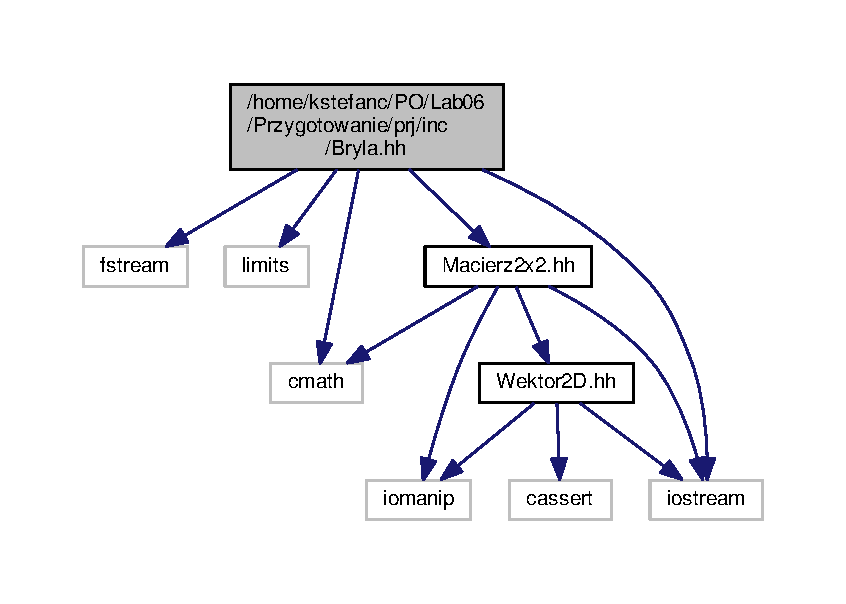
\includegraphics[width=350pt]{_bryla_8hh__incl}
\end{center}
\end{figure}
\subsection*{Classes}
\begin{DoxyCompactItemize}
\item 
class \hyperlink{class_bryla}{Bryla}
\begin{DoxyCompactList}\small\item\em Modeluje informacje dotyczace polozenia bryły. \end{DoxyCompactList}\end{DoxyCompactItemize}
\subsection*{Macros}
\begin{DoxyCompactItemize}
\item 
\hypertarget{_bryla_8hh_a0f96e3ce9bab3bd512fb07a5e2a41912}{\#define {\bfseries L\+I\+C\+Z\+B\+A\+\_\+\+B\+O\+K\+O\+W}~12}\label{_bryla_8hh_a0f96e3ce9bab3bd512fb07a5e2a41912}

\item 
\hypertarget{_bryla_8hh_aeedd3cc6d1b0749386c0d3174d8aabd7}{\#define {\bfseries L\+I\+C\+Z\+B\+A\+\_\+\+P\+U\+N\+K\+T\+O\+W}~8}\label{_bryla_8hh_aeedd3cc6d1b0749386c0d3174d8aabd7}

\end{DoxyCompactItemize}
\subsection*{Functions}
\begin{DoxyCompactItemize}
\item 
\hypertarget{_bryla_8hh_a2faaa91188cb3ab8157ae93ce45a7058}{std\+::ostream \& {\bfseries operator$<$$<$} (std\+::ostream \&Strm, const \hyperlink{class_bryla}{Bryla} \&Pr)}\label{_bryla_8hh_a2faaa91188cb3ab8157ae93ce45a7058}

\end{DoxyCompactItemize}


\subsection{Detailed Description}
Deklaracja klasy typu \hyperlink{class_bryla}{Bryla}. 

Plik zawiera deklaracje klasy \hyperlink{class_bryla}{Bryla} 
\hypertarget{lacze__do__gnuplota_8hh}{\section{/home/kstefanc/\+P\+O/\+Lab04/\+Lab/prj/inc/lacze\+\_\+do\+\_\+gnuplota.hh File Reference}
\label{lacze__do__gnuplota_8hh}\index{/home/kstefanc/\+P\+O/\+Lab04/\+Lab/prj/inc/lacze\+\_\+do\+\_\+gnuplota.\+hh@{/home/kstefanc/\+P\+O/\+Lab04/\+Lab/prj/inc/lacze\+\_\+do\+\_\+gnuplota.\+hh}}
}
{\ttfamily \#include $<$string$>$}\\*
{\ttfamily \#include $<$list$>$}\\*
{\ttfamily \#include $<$vector$>$}\\*
Include dependency graph for lacze\+\_\+do\+\_\+gnuplota.\+hh\+:\nopagebreak
\begin{figure}[H]
\begin{center}
\leavevmode
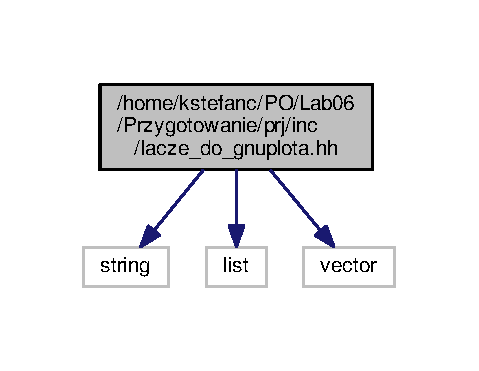
\includegraphics[width=230pt]{lacze__do__gnuplota_8hh__incl}
\end{center}
\end{figure}
\subsection*{Classes}
\begin{DoxyCompactItemize}
\item 
class \hyperlink{class_pz_g_1_1_info_pliku_do_rysowania}{Pz\+G\+::\+Info\+Pliku\+Do\+Rysowania}
\begin{DoxyCompactList}\small\item\em Zestaw informacji dotyczący pliku i sposobu rysowania. \end{DoxyCompactList}\item 
class \hyperlink{class_pz_g_1_1_lacze_do_g_n_u_plota}{Pz\+G\+::\+Lacze\+Do\+G\+N\+U\+Plota}
\begin{DoxyCompactList}\small\item\em Klasa realizuje interfejs do programu G\+N\+U\+Plot. \end{DoxyCompactList}\end{DoxyCompactItemize}
\subsection*{Namespaces}
\begin{DoxyCompactItemize}
\item 
 \hyperlink{namespace_pz_g}{Pz\+G}
\begin{DoxyCompactList}\small\item\em Moduł narzędzi umożliwiających połącznie z G\+N\+U\+Plotem. \end{DoxyCompactList}\end{DoxyCompactItemize}
\subsection*{Enumerations}
\begin{DoxyCompactItemize}
\item 
enum \hyperlink{namespace_pz_g_aeedae1ef10c66d720f9e89de408ca4ca}{Pz\+G\+::\+Tryb\+Rysowania} \{ {\bfseries T\+R\+\_\+2\+D}, 
{\bfseries T\+R\+\_\+3\+D}
 \}
\begin{DoxyCompactList}\small\item\em Określa tryb rysowania realizowanego przez program {\ttfamily gnuplot}. \end{DoxyCompactList}\item 
enum \hyperlink{namespace_pz_g_a705c92106f39b7d0c34a6739d10ff0b6}{Pz\+G\+::\+Rodzaj\+Rysowania} \{ {\bfseries R\+R\+\_\+\+Ciagly}, 
{\bfseries R\+R\+\_\+\+Punktowy}
 \}
\begin{DoxyCompactList}\small\item\em Sposób rysowania linii. \end{DoxyCompactList}\end{DoxyCompactItemize}


\subsection{Detailed Description}
Plik zawiera definicję klasy realizującej interfejs komunikacyjny do programu gnuplot. 
\hypertarget{_macierz2x2_8hh}{\section{/home/kstefanc/\+P\+O/\+Lab06/\+Przygotowanie/prj/inc/\+Macierz2x2.hh File Reference}
\label{_macierz2x2_8hh}\index{/home/kstefanc/\+P\+O/\+Lab06/\+Przygotowanie/prj/inc/\+Macierz2x2.\+hh@{/home/kstefanc/\+P\+O/\+Lab06/\+Przygotowanie/prj/inc/\+Macierz2x2.\+hh}}
}


Definicja klasy \hyperlink{class_macierz2x2}{Macierz2x2}.  


{\ttfamily \#include \char`\"{}Wektor2\+D.\+hh\char`\"{}}\\*
{\ttfamily \#include $<$iostream$>$}\\*
{\ttfamily \#include $<$iomanip$>$}\\*
{\ttfamily \#include $<$cmath$>$}\\*
Include dependency graph for Macierz2x2.\+hh\+:\nopagebreak
\begin{figure}[H]
\begin{center}
\leavevmode
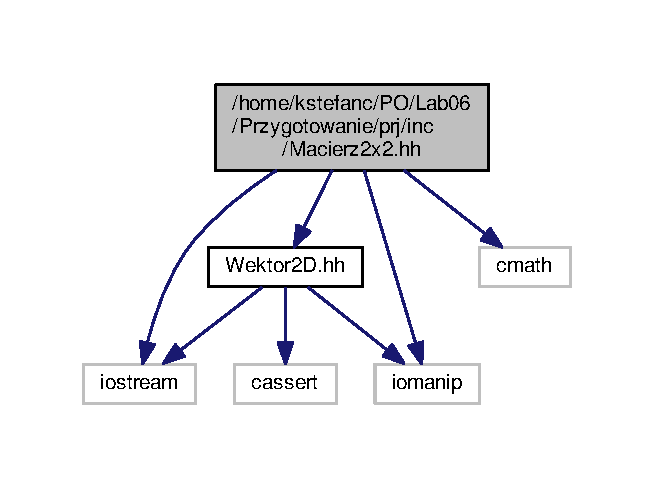
\includegraphics[width=314pt]{_macierz2x2_8hh__incl}
\end{center}
\end{figure}
This graph shows which files directly or indirectly include this file\+:
\nopagebreak
\begin{figure}[H]
\begin{center}
\leavevmode
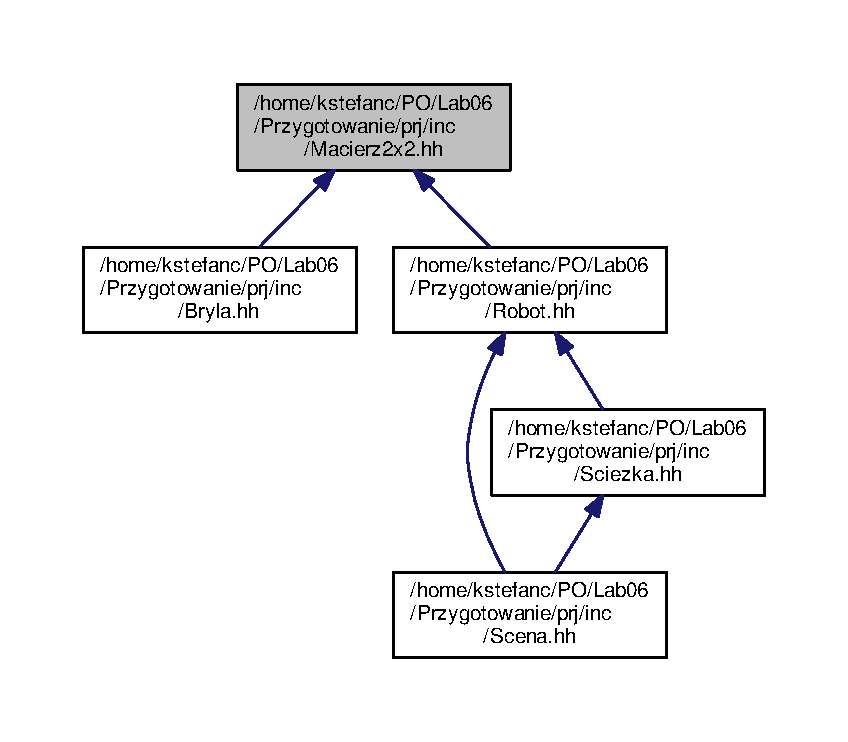
\includegraphics[width=350pt]{_macierz2x2_8hh__dep__incl}
\end{center}
\end{figure}
\subsection*{Classes}
\begin{DoxyCompactItemize}
\item 
class \hyperlink{class_macierz2x2}{Macierz2x2}
\begin{DoxyCompactList}\small\item\em Modeluje informacje dotyczace macierzy ktora jest uzywana do obrotu figury. \end{DoxyCompactList}\end{DoxyCompactItemize}
\subsection*{Macros}
\begin{DoxyCompactItemize}
\item 
\hypertarget{_macierz2x2_8hh_a9d01784f7ff1b3fd53cb75db78488adc}{\#define {\bfseries R\+O\+Z\+M\+I\+A\+R\+\_\+\+M\+A\+C\+I\+E\+R\+Z\+Y}~2}\label{_macierz2x2_8hh_a9d01784f7ff1b3fd53cb75db78488adc}

\end{DoxyCompactItemize}
\subsection*{Functions}
\begin{DoxyCompactItemize}
\item 
\hypertarget{_macierz2x2_8hh_aa3eba72acf9e09b901351ce2bc5edf2f}{std\+::ostream \& {\bfseries operator$<$$<$} (std\+::ostream \&Strm, const \hyperlink{class_macierz2x2}{Macierz2x2} \&Mac)}\label{_macierz2x2_8hh_aa3eba72acf9e09b901351ce2bc5edf2f}

\item 
\hypertarget{_macierz2x2_8hh_a41b60a94bb9873f185ec2fe49b19eed4}{std\+::istream \& {\bfseries operator$>$$>$} (std\+::istream \&Strm, \hyperlink{class_macierz2x2}{Macierz2x2} \&Mac)}\label{_macierz2x2_8hh_a41b60a94bb9873f185ec2fe49b19eed4}

\end{DoxyCompactItemize}


\subsection{Detailed Description}
Definicja klasy \hyperlink{class_macierz2x2}{Macierz2x2}. 

Plik zawiera kalse \hyperlink{class_macierz2x2}{Macierz2x2} 
\hypertarget{_objekt___graficzny_8hh}{\section{/home/kstefanc/\+P\+O/\+Lab06/\+Lab/prj/inc/\+Objekt\+\_\+\+Graficzny.hh File Reference}
\label{_objekt___graficzny_8hh}\index{/home/kstefanc/\+P\+O/\+Lab06/\+Lab/prj/inc/\+Objekt\+\_\+\+Graficzny.\+hh@{/home/kstefanc/\+P\+O/\+Lab06/\+Lab/prj/inc/\+Objekt\+\_\+\+Graficzny.\+hh}}
}


Definicja klasy \hyperlink{class_objekt___graficzny}{Objekt\+\_\+\+Graficzny}.  


{\ttfamily \#include \char`\"{}Zbior\+Wierzcholkow.\+hh\char`\"{}}\\*
{\ttfamily \#include $<$fstream$>$}\\*
{\ttfamily \#include $<$iostream$>$}\\*
{\ttfamily \#include $<$iomanip$>$}\\*
{\ttfamily \#include $<$cmath$>$}\\*
{\ttfamily \#include $<$vector$>$}\\*
Include dependency graph for Objekt\+\_\+\+Graficzny.\+hh\+:\nopagebreak
\begin{figure}[H]
\begin{center}
\leavevmode
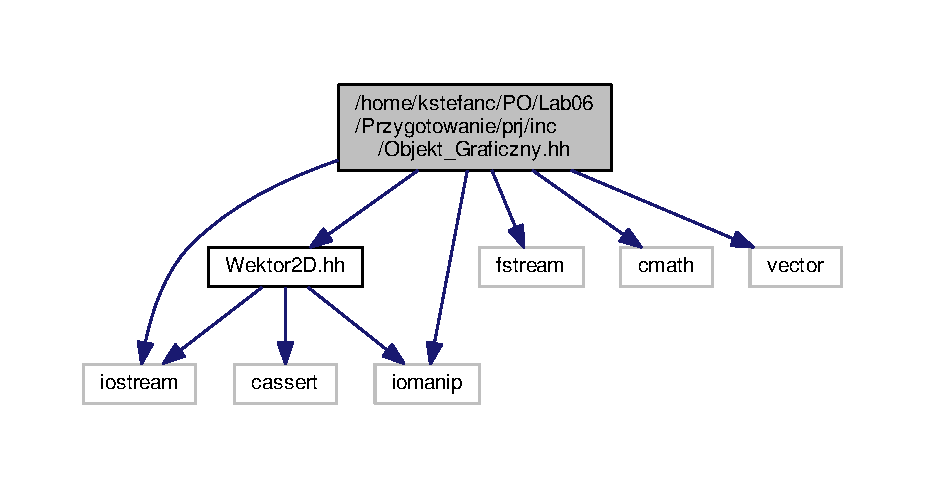
\includegraphics[width=350pt]{_objekt___graficzny_8hh__incl}
\end{center}
\end{figure}
This graph shows which files directly or indirectly include this file\+:\nopagebreak
\begin{figure}[H]
\begin{center}
\leavevmode
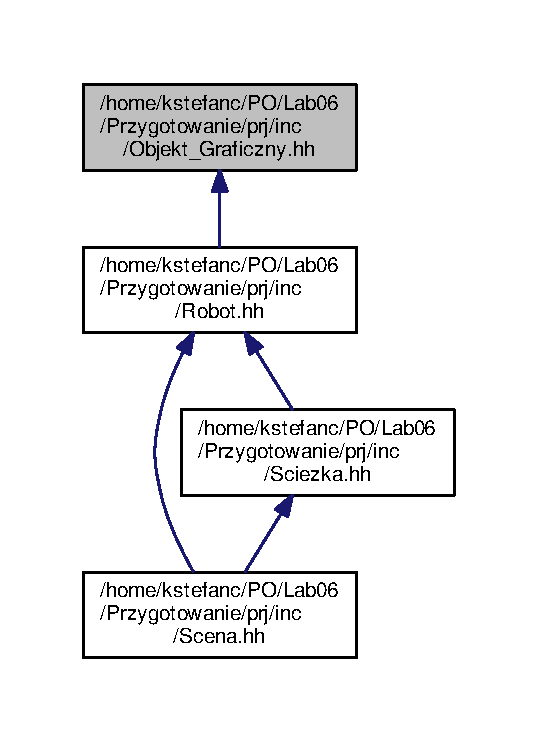
\includegraphics[width=271pt]{_objekt___graficzny_8hh__dep__incl}
\end{center}
\end{figure}
\subsection*{Classes}
\begin{DoxyCompactItemize}
\item 
class \hyperlink{class_objekt___graficzny}{Objekt\+\_\+\+Graficzny}
\begin{DoxyCompactList}\small\item\em Modeluje informacje dotyczace \hyperlink{class_objekt___graficzny}{Objekt\+\_\+\+Graficzny}. \end{DoxyCompactList}\end{DoxyCompactItemize}
\subsection*{Functions}
\begin{DoxyCompactItemize}
\item 
\hypertarget{_objekt___graficzny_8hh_a43ce12bd48e47ba41645772340e7103b}{std\+::ostream \& \hyperlink{_objekt___graficzny_8hh_a43ce12bd48e47ba41645772340e7103b}{operator$<$$<$} (std\+::ostream \&Strm, const \hyperlink{class_objekt___graficzny}{Objekt\+\_\+\+Graficzny} \&Obj\+\_\+\+Graf)}\label{_objekt___graficzny_8hh_a43ce12bd48e47ba41645772340e7103b}

\begin{DoxyCompactList}\small\item\em Wyswietla współrzędne wierzchołków ścieżki. \end{DoxyCompactList}\end{DoxyCompactItemize}


\subsection{Detailed Description}
Definicja klasy \hyperlink{class_objekt___graficzny}{Objekt\+\_\+\+Graficzny}. 

Plik zawiera kalse \hyperlink{class_objekt___graficzny}{Objekt\+\_\+\+Graficzny} 
\hypertarget{_robot_8hh}{\section{/home/kstefanc/\+P\+O/\+Lab06/\+Przygotowanie/prj/inc/\+Robot.hh File Reference}
\label{_robot_8hh}\index{/home/kstefanc/\+P\+O/\+Lab06/\+Przygotowanie/prj/inc/\+Robot.\+hh@{/home/kstefanc/\+P\+O/\+Lab06/\+Przygotowanie/prj/inc/\+Robot.\+hh}}
}


Definicja klasy \hyperlink{class_robot}{Robot}.  


{\ttfamily \#include \char`\"{}Macierz2x2.\+hh\char`\"{}}\\*
{\ttfamily \#include \char`\"{}Objekt\+\_\+\+Graficzny.\+hh\char`\"{}}\\*
{\ttfamily \#include $<$fstream$>$}\\*
{\ttfamily \#include $<$iostream$>$}\\*
{\ttfamily \#include $<$iomanip$>$}\\*
{\ttfamily \#include $<$cmath$>$}\\*
Include dependency graph for Robot.\+hh\+:
\nopagebreak
\begin{figure}[H]
\begin{center}
\leavevmode
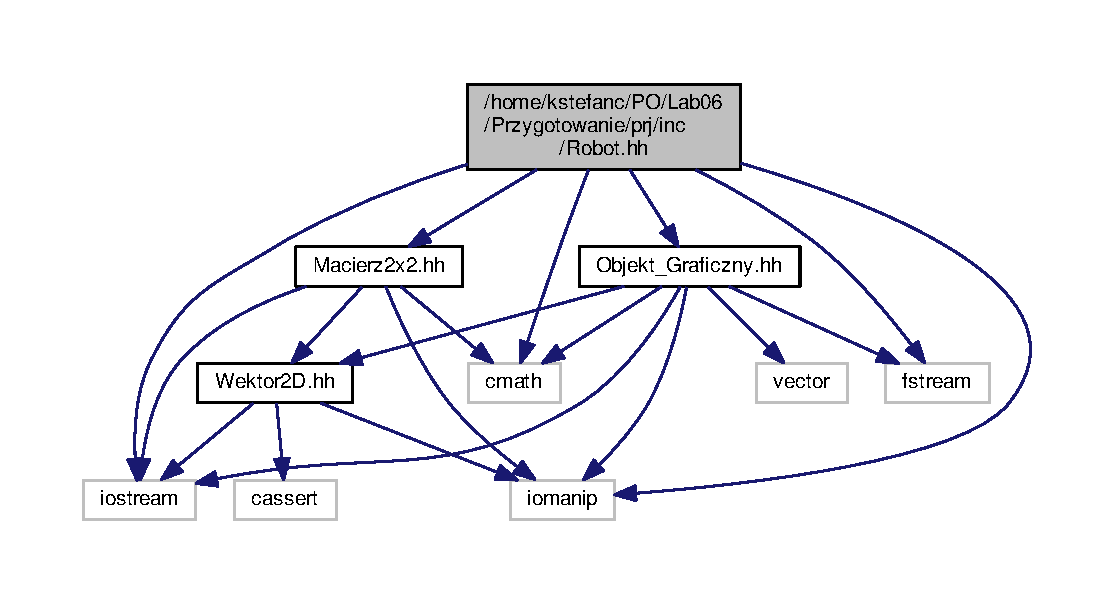
\includegraphics[width=350pt]{_robot_8hh__incl}
\end{center}
\end{figure}
This graph shows which files directly or indirectly include this file\+:
\nopagebreak
\begin{figure}[H]
\begin{center}
\leavevmode
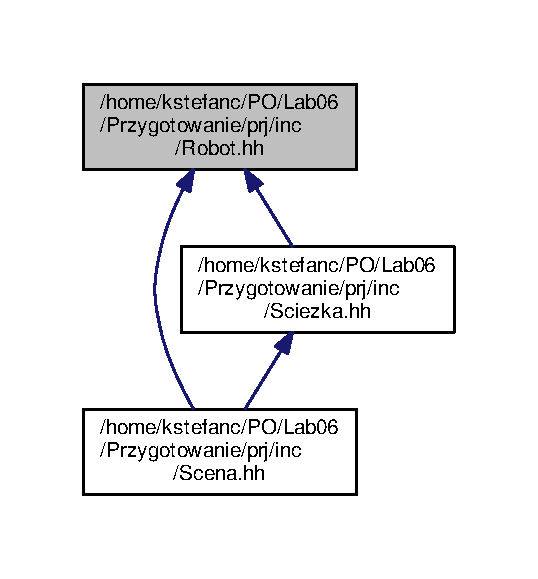
\includegraphics[width=258pt]{_robot_8hh__dep__incl}
\end{center}
\end{figure}
\subsection*{Classes}
\begin{DoxyCompactItemize}
\item 
class \hyperlink{class_robot}{Robot}
\begin{DoxyCompactList}\small\item\em Modeluje informacje dotyczace prostokąta. \end{DoxyCompactList}\end{DoxyCompactItemize}
\subsection*{Macros}
\begin{DoxyCompactItemize}
\item 
\hypertarget{_robot_8hh_aeedd3cc6d1b0749386c0d3174d8aabd7}{\#define {\bfseries L\+I\+C\+Z\+B\+A\+\_\+\+P\+U\+N\+K\+T\+O\+W}~6}\label{_robot_8hh_aeedd3cc6d1b0749386c0d3174d8aabd7}

\end{DoxyCompactItemize}
\subsection*{Functions}
\begin{DoxyCompactItemize}
\item 
std\+::ostream \& \hyperlink{_robot_8hh_aacddbdd412cecfab568c49b6f389bf42}{operator$<$$<$} (std\+::ostream \&Strm, const \hyperlink{class_robot}{Robot} \&Rob)
\begin{DoxyCompactList}\small\item\em Wyswietla współrzędne wierzchołków względem siebie. \end{DoxyCompactList}\end{DoxyCompactItemize}


\subsection{Detailed Description}
Definicja klasy \hyperlink{class_robot}{Robot}. 

Plik zawiera kalse \hyperlink{class_robot}{Robot} 

\subsection{Function Documentation}
\hypertarget{_robot_8hh_aacddbdd412cecfab568c49b6f389bf42}{\index{Robot.\+hh@{Robot.\+hh}!operator$<$$<$@{operator$<$$<$}}
\index{operator$<$$<$@{operator$<$$<$}!Robot.\+hh@{Robot.\+hh}}
\subsubsection[{operator$<$$<$}]{\setlength{\rightskip}{0pt plus 5cm}std\+::ostream\& operator$<$$<$ (
\begin{DoxyParamCaption}
\item[{std\+::ostream \&}]{Strm, }
\item[{const {\bf Robot} \&}]{Rob}
\end{DoxyParamCaption}
)}}\label{_robot_8hh_aacddbdd412cecfab568c49b6f389bf42}


Wyswietla współrzędne wierzchołków względem siebie. 

Uwzględnia kąt a nie uwzględnia przesunięcia. 
\hypertarget{_scena_8hh}{\section{/home/kstefanc/\+P\+O/\+Lab07/\+Lab/prj/inc/\+Scena.hh File Reference}
\label{_scena_8hh}\index{/home/kstefanc/\+P\+O/\+Lab07/\+Lab/prj/inc/\+Scena.\+hh@{/home/kstefanc/\+P\+O/\+Lab07/\+Lab/prj/inc/\+Scena.\+hh}}
}


Definicja klasy \hyperlink{class_scena}{Scena}.  


{\ttfamily \#include \char`\"{}lacze\+\_\+do\+\_\+gnuplota.\+hh\char`\"{}}\\*
{\ttfamily \#include \char`\"{}Robot.\+hh\char`\"{}}\\*
{\ttfamily \#include \char`\"{}Przeszkoda.\+hh\char`\"{}}\\*
{\ttfamily \#include \char`\"{}Zbior\+Wierzcholkow.\+hh\char`\"{}}\\*
{\ttfamily \#include \char`\"{}Sciezka.\+hh\char`\"{}}\\*
{\ttfamily \#include $<$fstream$>$}\\*
{\ttfamily \#include $<$iostream$>$}\\*
{\ttfamily \#include $<$iomanip$>$}\\*
{\ttfamily \#include $<$cmath$>$}\\*
{\ttfamily \#include $<$vector$>$}\\*
{\ttfamily \#include $<$list$>$}\\*
{\ttfamily \#include $<$memory$>$}\\*
Include dependency graph for Scena.\+hh\+:\nopagebreak
\begin{figure}[H]
\begin{center}
\leavevmode
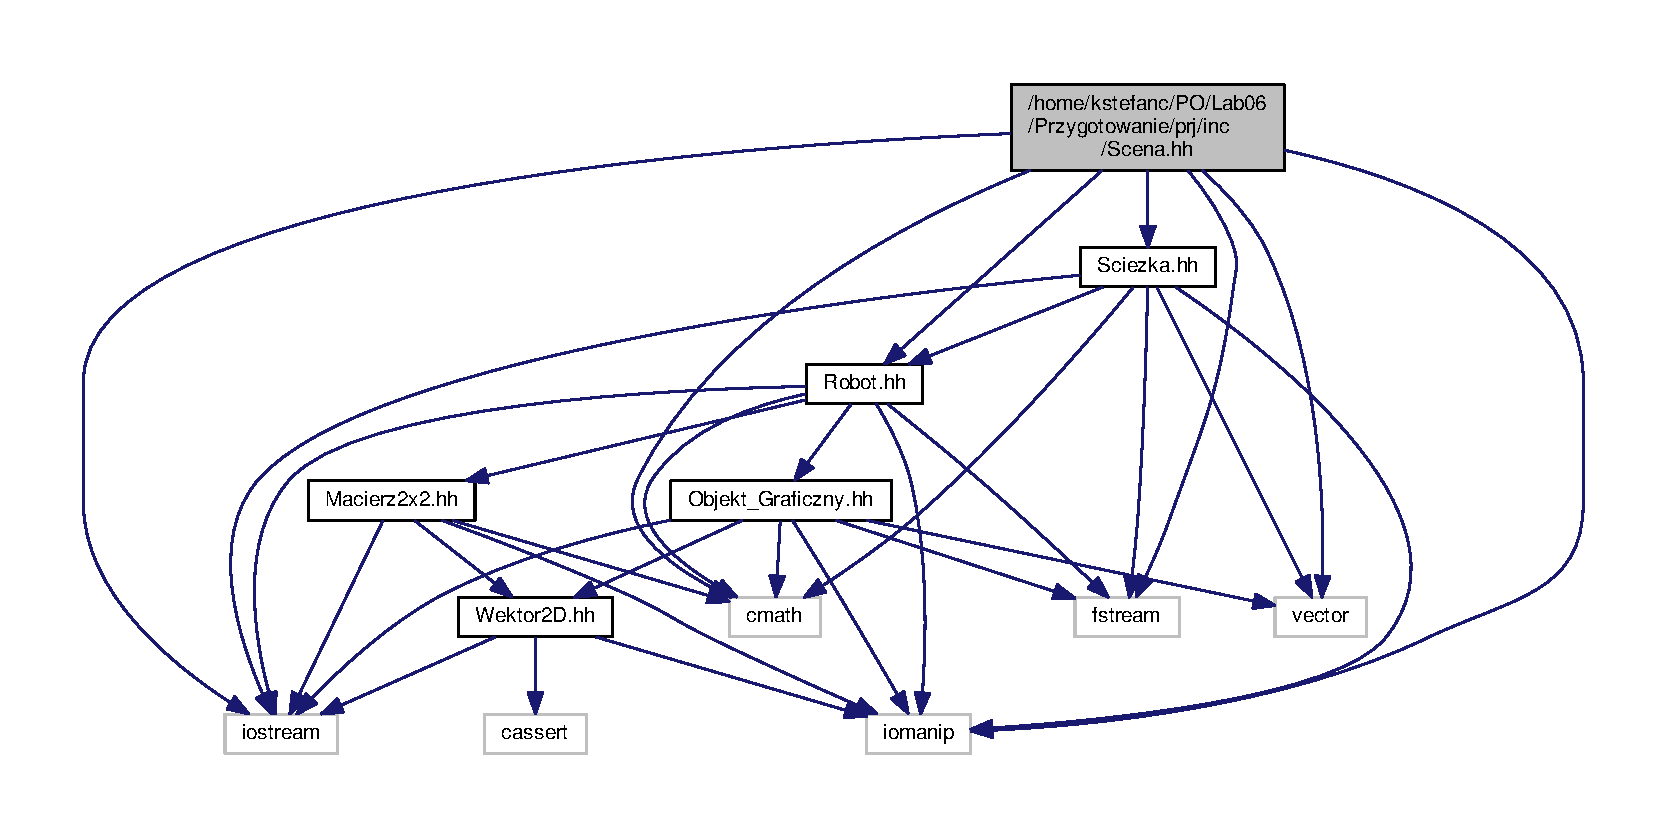
\includegraphics[width=350pt]{_scena_8hh__incl}
\end{center}
\end{figure}
\subsection*{Classes}
\begin{DoxyCompactItemize}
\item 
class \hyperlink{class_scena}{Scena}
\begin{DoxyCompactList}\small\item\em Modeluje informacje dotyczace Sceny. \end{DoxyCompactList}\end{DoxyCompactItemize}


\subsection{Detailed Description}
Definicja klasy \hyperlink{class_scena}{Scena}. 

Plik zawiera kalse \hyperlink{class_scena}{Scena} 
\hypertarget{_sciezka_8hh}{\section{/home/kstefanc/\+P\+O/\+Lab06/\+Lab/prj/inc/\+Sciezka.hh File Reference}
\label{_sciezka_8hh}\index{/home/kstefanc/\+P\+O/\+Lab06/\+Lab/prj/inc/\+Sciezka.\+hh@{/home/kstefanc/\+P\+O/\+Lab06/\+Lab/prj/inc/\+Sciezka.\+hh}}
}


Definicja klasy \hyperlink{class_sciezka}{Sciezka}.  


{\ttfamily \#include \char`\"{}Robot.\+hh\char`\"{}}\\*
{\ttfamily \#include $<$unistd.\+h$>$}\\*
{\ttfamily \#include $<$fstream$>$}\\*
{\ttfamily \#include $<$limits$>$}\\*
{\ttfamily \#include $<$iostream$>$}\\*
{\ttfamily \#include $<$iomanip$>$}\\*
{\ttfamily \#include $<$cmath$>$}\\*
{\ttfamily \#include $<$vector$>$}\\*
Include dependency graph for Sciezka.\+hh\+:\nopagebreak
\begin{figure}[H]
\begin{center}
\leavevmode
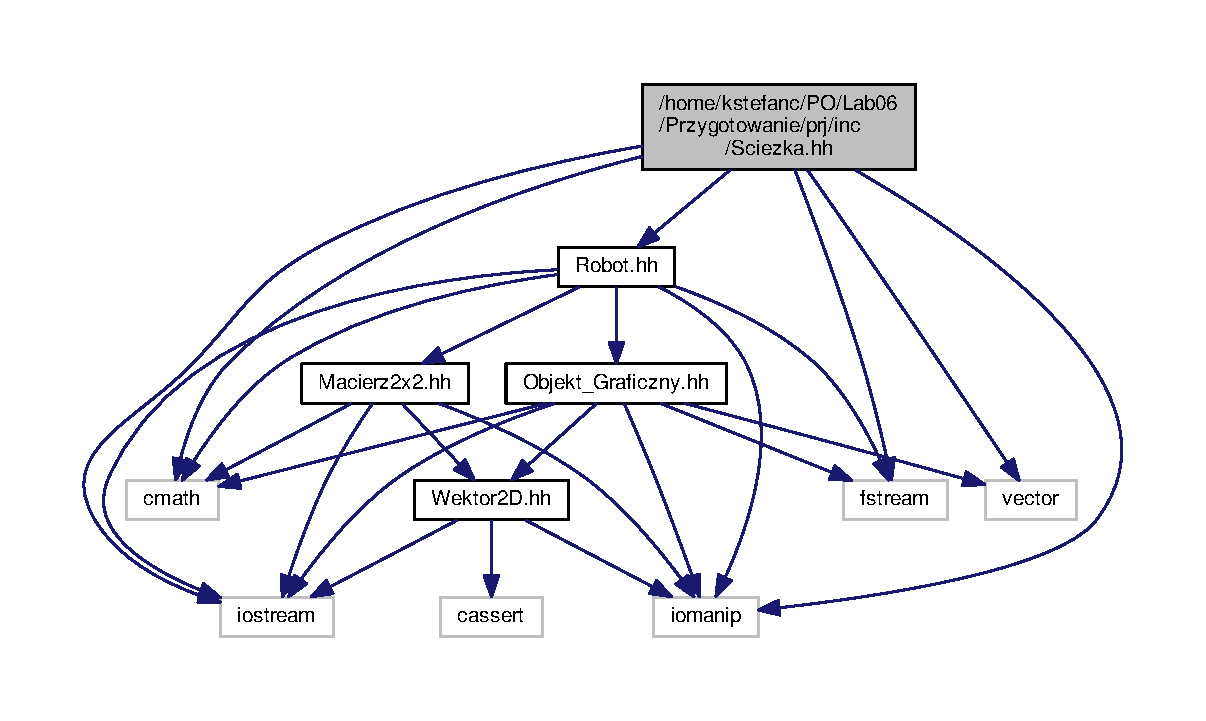
\includegraphics[width=350pt]{_sciezka_8hh__incl}
\end{center}
\end{figure}
This graph shows which files directly or indirectly include this file\+:\nopagebreak
\begin{figure}[H]
\begin{center}
\leavevmode
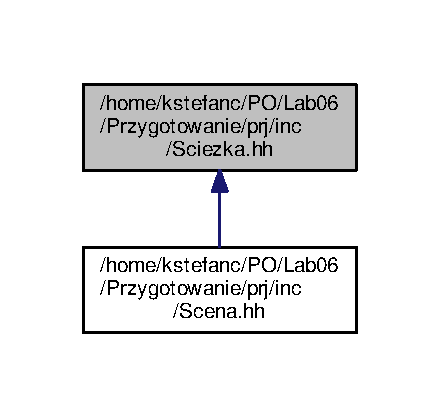
\includegraphics[width=211pt]{_sciezka_8hh__dep__incl}
\end{center}
\end{figure}
\subsection*{Classes}
\begin{DoxyCompactItemize}
\item 
class \hyperlink{class_sciezka}{Sciezka}
\begin{DoxyCompactList}\small\item\em Modeluje informacje dotyczace Ścieżki. \end{DoxyCompactList}\end{DoxyCompactItemize}


\subsection{Detailed Description}
Definicja klasy \hyperlink{class_sciezka}{Sciezka}. 

Plik zawiera kalse \hyperlink{class_sciezka}{Sciezka} 
\hypertarget{_wektor2_d_8hh}{\section{/home/kstefanc/\+P\+O/\+Lab04/\+Lab/prj/inc/\+Wektor2\+D.hh File Reference}
\label{_wektor2_d_8hh}\index{/home/kstefanc/\+P\+O/\+Lab04/\+Lab/prj/inc/\+Wektor2\+D.\+hh@{/home/kstefanc/\+P\+O/\+Lab04/\+Lab/prj/inc/\+Wektor2\+D.\+hh}}
}


Definicja kalsy typu \hyperlink{class_wektor2_d}{Wektor2\+D}.  


{\ttfamily \#include $<$iostream$>$}\\*
{\ttfamily \#include $<$iomanip$>$}\\*
Include dependency graph for Wektor2\+D.\+hh\+:\nopagebreak
\begin{figure}[H]
\begin{center}
\leavevmode
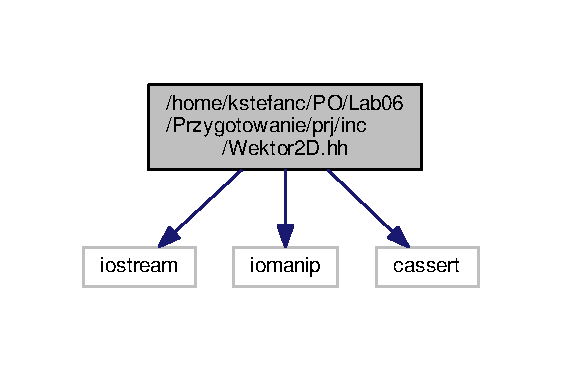
\includegraphics[width=211pt]{_wektor2_d_8hh__incl}
\end{center}
\end{figure}
This graph shows which files directly or indirectly include this file\+:\nopagebreak
\begin{figure}[H]
\begin{center}
\leavevmode
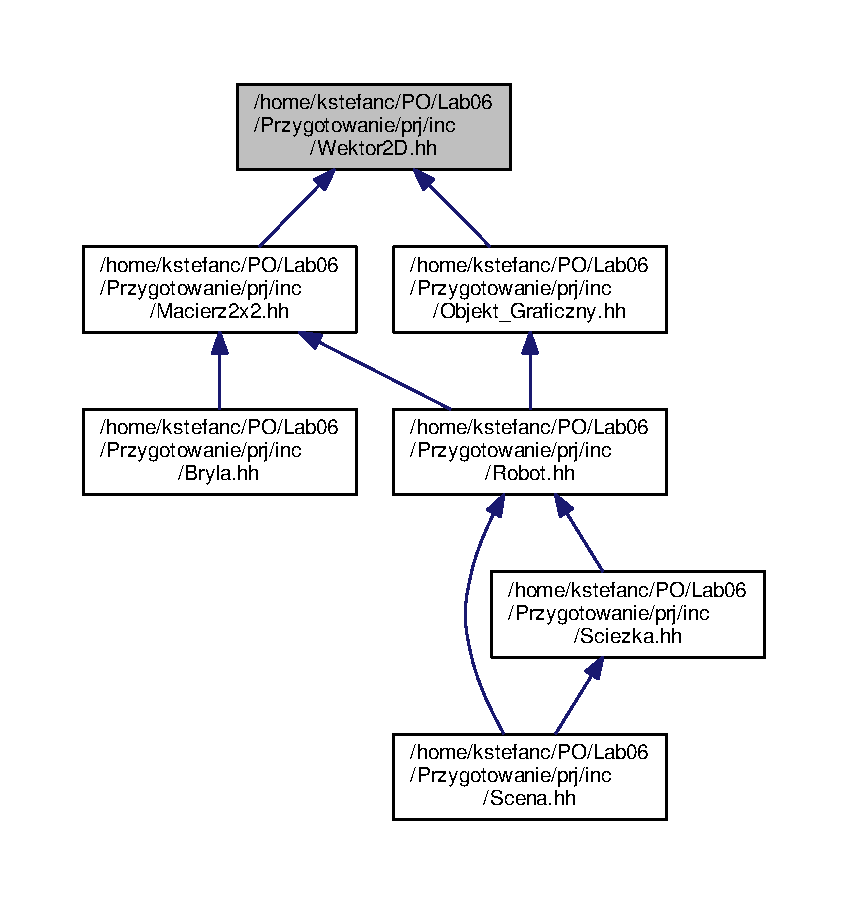
\includegraphics[width=211pt]{_wektor2_d_8hh__dep__incl}
\end{center}
\end{figure}
\subsection*{Classes}
\begin{DoxyCompactItemize}
\item 
class \hyperlink{class_wektor2_d}{Wektor2\+D}
\begin{DoxyCompactList}\small\item\em Modeluje informacje dotyczace wektora. \end{DoxyCompactList}\end{DoxyCompactItemize}
\subsection*{Functions}
\begin{DoxyCompactItemize}
\item 
std\+::istream \& \hyperlink{_wektor2_d_8hh_add22cd44a5725ef9bd7ec6954a40c23c}{operator$>$$>$} (std\+::istream \&Strm, \hyperlink{class_wektor2_d}{Wektor2\+D} \&Wek)
\begin{DoxyCompactList}\small\item\em Wczytuje współrzędne wektora. \end{DoxyCompactList}\item 
std\+::ostream \& \hyperlink{_wektor2_d_8hh_a441a89c1708691259d6afd762fdfada2}{operator$<$$<$} (std\+::ostream \&Strm, const \hyperlink{class_wektor2_d}{Wektor2\+D} \&Wek)
\begin{DoxyCompactList}\small\item\em Wyswietla współrzędne wektora. \end{DoxyCompactList}\end{DoxyCompactItemize}


\subsection{Detailed Description}
Definicja kalsy typu \hyperlink{class_wektor2_d}{Wektor2\+D}. 

Plik zawiera deklaracje klasy \hyperlink{class_wektor2_d}{Wektor2\+D} i przeciążeń operatorów cout i cin dla klasy \hyperlink{class_wektor2_d}{Wektor2\+D} 

\subsection{Function Documentation}
\hypertarget{_wektor2_d_8hh_a441a89c1708691259d6afd762fdfada2}{\index{Wektor2\+D.\+hh@{Wektor2\+D.\+hh}!operator$<$$<$@{operator$<$$<$}}
\index{operator$<$$<$@{operator$<$$<$}!Wektor2\+D.\+hh@{Wektor2\+D.\+hh}}
\subsubsection[{operator$<$$<$}]{\setlength{\rightskip}{0pt plus 5cm}std\+::ostream\& operator$<$$<$ (
\begin{DoxyParamCaption}
\item[{std\+::ostream \&}]{Strm, }
\item[{const {\bf Wektor2\+D} \&}]{Wek}
\end{DoxyParamCaption}
)}}\label{_wektor2_d_8hh_a441a89c1708691259d6afd762fdfada2}


Wyswietla współrzędne wektora. 

Współrzędne są zwracane w kolejności x (znak tabulacji) y \hypertarget{_wektor2_d_8hh_add22cd44a5725ef9bd7ec6954a40c23c}{\index{Wektor2\+D.\+hh@{Wektor2\+D.\+hh}!operator$>$$>$@{operator$>$$>$}}
\index{operator$>$$>$@{operator$>$$>$}!Wektor2\+D.\+hh@{Wektor2\+D.\+hh}}
\subsubsection[{operator$>$$>$}]{\setlength{\rightskip}{0pt plus 5cm}std\+::istream\& operator$>$$>$ (
\begin{DoxyParamCaption}
\item[{std\+::istream \&}]{Strm, }
\item[{{\bf Wektor2\+D} \&}]{Wek}
\end{DoxyParamCaption}
)}}\label{_wektor2_d_8hh_add22cd44a5725ef9bd7ec6954a40c23c}


Wczytuje współrzędne wektora. 

Współrzędne są pobierane w kolejności x potem y 
%--- End generated contents ---

% Index
\newpage
\phantomsection
\addcontentsline{toc}{chapter}{Index}
\printindex

\end{document}
